% Options for packages loaded elsewhere
\PassOptionsToPackage{unicode}{hyperref}
\PassOptionsToPackage{hyphens}{url}
\PassOptionsToPackage{dvipsnames,svgnames*,x11names*}{xcolor}
%
\documentclass[
  10pt,
]{article}
\usepackage{lmodern}
\usepackage{amssymb,amsmath}
\usepackage{ifxetex,ifluatex}
\ifnum 0\ifxetex 1\fi\ifluatex 1\fi=0 % if pdftex
  \usepackage[T1]{fontenc}
  \usepackage[utf8]{inputenc}
  \usepackage{textcomp} % provide euro and other symbols
\else % if luatex or xetex
  \usepackage{unicode-math}
  \defaultfontfeatures{Scale=MatchLowercase}
  \defaultfontfeatures[\rmfamily]{Ligatures=TeX,Scale=1}
\fi
% Use upquote if available, for straight quotes in verbatim environments
\IfFileExists{upquote.sty}{\usepackage{upquote}}{}
\IfFileExists{microtype.sty}{% use microtype if available
  \usepackage[]{microtype}
  \UseMicrotypeSet[protrusion]{basicmath} % disable protrusion for tt fonts
}{}
\makeatletter
\@ifundefined{KOMAClassName}{% if non-KOMA class
  \IfFileExists{parskip.sty}{%
    \usepackage{parskip}
  }{% else
    \setlength{\parindent}{0pt}
    \setlength{\parskip}{6pt plus 2pt minus 1pt}}
}{% if KOMA class
  \KOMAoptions{parskip=half}}
\makeatother
\usepackage{xcolor}
\IfFileExists{xurl.sty}{\usepackage{xurl}}{} % add URL line breaks if available
\IfFileExists{bookmark.sty}{\usepackage{bookmark}}{\usepackage{hyperref}}
\hypersetup{
  colorlinks=true,
  linkcolor=red,
  filecolor=Maroon,
  citecolor=Blue,
  urlcolor=blue,
  pdfcreator={LaTeX via pandoc}}
\urlstyle{same} % disable monospaced font for URLs
\usepackage[margin=1in]{geometry}
\usepackage{color}
\usepackage{fancyvrb}
\newcommand{\VerbBar}{|}
\newcommand{\VERB}{\Verb[commandchars=\\\{\}]}
\DefineVerbatimEnvironment{Highlighting}{Verbatim}{commandchars=\\\{\}}
% Add ',fontsize=\small' for more characters per line
\usepackage{framed}
\definecolor{shadecolor}{RGB}{248,248,248}
\newenvironment{Shaded}{\begin{snugshade}}{\end{snugshade}}
\newcommand{\AlertTok}[1]{\textcolor[rgb]{0.94,0.16,0.16}{#1}}
\newcommand{\AnnotationTok}[1]{\textcolor[rgb]{0.56,0.35,0.01}{\textbf{\textit{#1}}}}
\newcommand{\AttributeTok}[1]{\textcolor[rgb]{0.77,0.63,0.00}{#1}}
\newcommand{\BaseNTok}[1]{\textcolor[rgb]{0.00,0.00,0.81}{#1}}
\newcommand{\BuiltInTok}[1]{#1}
\newcommand{\CharTok}[1]{\textcolor[rgb]{0.31,0.60,0.02}{#1}}
\newcommand{\CommentTok}[1]{\textcolor[rgb]{0.56,0.35,0.01}{\textit{#1}}}
\newcommand{\CommentVarTok}[1]{\textcolor[rgb]{0.56,0.35,0.01}{\textbf{\textit{#1}}}}
\newcommand{\ConstantTok}[1]{\textcolor[rgb]{0.00,0.00,0.00}{#1}}
\newcommand{\ControlFlowTok}[1]{\textcolor[rgb]{0.13,0.29,0.53}{\textbf{#1}}}
\newcommand{\DataTypeTok}[1]{\textcolor[rgb]{0.13,0.29,0.53}{#1}}
\newcommand{\DecValTok}[1]{\textcolor[rgb]{0.00,0.00,0.81}{#1}}
\newcommand{\DocumentationTok}[1]{\textcolor[rgb]{0.56,0.35,0.01}{\textbf{\textit{#1}}}}
\newcommand{\ErrorTok}[1]{\textcolor[rgb]{0.64,0.00,0.00}{\textbf{#1}}}
\newcommand{\ExtensionTok}[1]{#1}
\newcommand{\FloatTok}[1]{\textcolor[rgb]{0.00,0.00,0.81}{#1}}
\newcommand{\FunctionTok}[1]{\textcolor[rgb]{0.00,0.00,0.00}{#1}}
\newcommand{\ImportTok}[1]{#1}
\newcommand{\InformationTok}[1]{\textcolor[rgb]{0.56,0.35,0.01}{\textbf{\textit{#1}}}}
\newcommand{\KeywordTok}[1]{\textcolor[rgb]{0.13,0.29,0.53}{\textbf{#1}}}
\newcommand{\NormalTok}[1]{#1}
\newcommand{\OperatorTok}[1]{\textcolor[rgb]{0.81,0.36,0.00}{\textbf{#1}}}
\newcommand{\OtherTok}[1]{\textcolor[rgb]{0.56,0.35,0.01}{#1}}
\newcommand{\PreprocessorTok}[1]{\textcolor[rgb]{0.56,0.35,0.01}{\textit{#1}}}
\newcommand{\RegionMarkerTok}[1]{#1}
\newcommand{\SpecialCharTok}[1]{\textcolor[rgb]{0.00,0.00,0.00}{#1}}
\newcommand{\SpecialStringTok}[1]{\textcolor[rgb]{0.31,0.60,0.02}{#1}}
\newcommand{\StringTok}[1]{\textcolor[rgb]{0.31,0.60,0.02}{#1}}
\newcommand{\VariableTok}[1]{\textcolor[rgb]{0.00,0.00,0.00}{#1}}
\newcommand{\VerbatimStringTok}[1]{\textcolor[rgb]{0.31,0.60,0.02}{#1}}
\newcommand{\WarningTok}[1]{\textcolor[rgb]{0.56,0.35,0.01}{\textbf{\textit{#1}}}}
\usepackage{graphicx,grffile}
\makeatletter
\def\maxwidth{\ifdim\Gin@nat@width>\linewidth\linewidth\else\Gin@nat@width\fi}
\def\maxheight{\ifdim\Gin@nat@height>\textheight\textheight\else\Gin@nat@height\fi}
\makeatother
% Scale images if necessary, so that they will not overflow the page
% margins by default, and it is still possible to overwrite the defaults
% using explicit options in \includegraphics[width, height, ...]{}
\setkeys{Gin}{width=\maxwidth,height=\maxheight,keepaspectratio}
% Set default figure placement to htbp
\makeatletter
\def\fps@figure{htbp}
\makeatother
\setlength{\emergencystretch}{3em} % prevent overfull lines
\providecommand{\tightlist}{%
  \setlength{\itemsep}{0pt}\setlength{\parskip}{0pt}}
\setcounter{secnumdepth}{5}
\usepackage{placeins}
\usepackage{fancyhdr}
\usepackage{setspace}
\onehalfspacing
\usepackage{pdfpages}
\usepackage{graphicx}
\usepackage{chngcntr}
\usepackage{subfig}
\usepackage{float}
\usepackage{ulem}
\usepackage{lscape}
\usepackage[utf8]{inputenc}
\newcommand{\blandscape}{\begin{landscape}}
\newcommand{\elandscape}{\end{landscape}}
\newcommand{\onlythepage}{\arabic{page}}
\newcommand*{\secref}[1]{Section~\ref{#1}}
\raggedbottom
\usepackage{amsmath}
\usepackage{hyperref}
\usepackage{amssymb}
\usepackage[greek,english]{babel}
\usepackage{enumerate}
\newcommand{\qed}{\hfill $\blacksquare$}
\renewcommand{\thepage}{(\thesection):\arabic{page}}
\usepackage{tcolorbox}
\tcbuselibrary{theorems}
\newtcbtheorem[number within=section]{mytheo}{Box}{colback=green!5,colframe=green!35!black,fonttitle=\bfseries}{th}

\author{}
\date{\vspace{-2.5em}}

\begin{document}

\pagenumbering{gobble}

\begin{centering}

\vspace{2 cm}

\Large

{\bf Økonometri I}

\vspace{2 cm}

\Large


\vspace{2 cm}

\normalsize


\vspace{12 cm}

\normalsize
Aalborg University Business School \\
Kasper Kann og Daniel Behr \\
Student ID: 20134818 og 20195227 \\
juli 2021

\vspace{2 cm}



\vspace{2 cm}


\end{centering}

\newpage

\pagestyle{fancy}

\fancyhead[LE,RO]{}
\fancyhead[LO,RE]{}

\renewcommand{\headrulewidth}{0.4pt}
\renewcommand{\footrulewidth}{0pt}

\pagenumbering{roman}

\FloatBarrier
\newpage

\FloatBarrier
\newpage

\fancyhead[CO,CE]{Indholdsfortegnelse}

\setcounter{tocdepth}{4}

\tableofcontents

\newpage
\FloatBarrier

\pagenumbering{arabic}

\FloatBarrier

\fancyhead[CO,CE]{Økonometri I}
\rfoot{\textit{\copyright\ Kann og Behr \ 2021}}

\includepdf[pages=1,pagecommand=\section{Eksamensopgave 1}, offset=0 -3cm]{opgave1}

\hypertarget{estimer-modellen-vha.-ols.-kommenter-puxe5-outputtet-og-fortolk-resultaterne.}{%
\subsection{Estimer modellen vha. OLS. Kommenter på outputtet og fortolk
resultaterne.}\label{estimer-modellen-vha.-ols.-kommenter-puxe5-outputtet-og-fortolk-resultaterne.}}

\leavevmode

Opstiller modellen vha OLS., som vi har udledt i
\hyperref[sec:OLS]{Appendix 1 - OLS}:
\[ log(salary) = \beta_0+\beta_1educ+\beta_2log(salbeginn)+\beta_3male+\beta_4minority\]
Opstiller model i R og udfører summary for at få estimater.

\begin{Shaded}
\begin{Highlighting}[]
\NormalTok{data1 <-}\StringTok{ }\KeywordTok{read_csv}\NormalTok{(}\StringTok{"C:/Users/Kann/Dropbox/Uni/Okonometri/data1.csv"}\NormalTok{)}
\NormalTok{model <-}\StringTok{ }\KeywordTok{lm}\NormalTok{(lsalary }\OperatorTok{~}\StringTok{ }\NormalTok{educ }\OperatorTok{+}\StringTok{ }\NormalTok{lsalbeginn }\OperatorTok{+}\StringTok{ }\NormalTok{male }\OperatorTok{+}\StringTok{ }\NormalTok{minority, }\DataTypeTok{data =}\NormalTok{ data1)}
\NormalTok{reg_}\DecValTok{1}\NormalTok{ <-}\StringTok{ }\KeywordTok{summary}\NormalTok{(model)}
\NormalTok{reg_}\DecValTok{1}
\CommentTok{## }
\CommentTok{## Call:}
\CommentTok{## lm(formula = lsalary ~ educ + lsalbeginn + male + minority, data = data1)}
\CommentTok{## }
\CommentTok{## Residuals:}
\CommentTok{##      Min       1Q   Median       3Q      Max }
\CommentTok{## -0.42452 -0.11908 -0.01378  0.10599  0.90025 }
\CommentTok{## }
\CommentTok{## Coefficients:}
\CommentTok{##              Estimate Std. Error t value Pr(>|t|)    }
\CommentTok{## (Intercept)  0.856040   0.083361  10.269  < 2e-16 ***}
\CommentTok{## educ         0.022264   0.004152   5.363  1.4e-07 ***}
\CommentTok{## lsalbeginn   0.820838   0.039915  20.565  < 2e-16 ***}
\CommentTok{## male         0.028855   0.021762   1.326    0.186    }
\CommentTok{## minority    -0.030720   0.021712  -1.415    0.158    }
\CommentTok{## ---}
\CommentTok{## Signif. codes:  0 '***' 0.001 '**' 0.01 '*' 0.05 '.' 0.1 ' ' 1}
\CommentTok{## }
\CommentTok{## Residual standard error: 0.1741 on 396 degrees of freedom}
\CommentTok{## Multiple R-squared:  0.7953, Adjusted R-squared:  0.7932 }
\CommentTok{## F-statistic: 384.7 on 4 and 396 DF,  p-value: < 2.2e-16}
\end{Highlighting}
\end{Shaded}

\textbf{Intercept:}\\
Vi kan se at interceptet er 0.85, og da vi har to dummy variable (male
og minority), så er det intercept for referencegruppen. I vores model er
referencegruppen kvinder, som ikke er en del af minoriteten.\\
\newpage

\textbf{Education:}\\
Vi kan fra vores model se at dataen for uddannelse er på level form,
hvorimod løn er på log form. Det betyder at vi skal gange \(β_1\) med
100, og så får vi 2.2\%. Det betyder at lønnen stiger med 2.2\% ved et
extra års uddannelse. Dette er kun et estimat, og vi kan beregne den
rette procentvise effekt med formlen: ~
\[\%\Delta\hat{y}=100*(exp(\hat{\beta_2})-1)\] udregnes i R:

\begin{Shaded}
\begin{Highlighting}[]
\DecValTok{100}\OperatorTok{*}\NormalTok{(}\KeywordTok{exp}\NormalTok{(reg_}\DecValTok{1}\OperatorTok{$}\NormalTok{coefficients[}\DecValTok{2}\NormalTok{,}\DecValTok{1}\NormalTok{])}\OperatorTok{-}\DecValTok{1}\NormalTok{)}
\CommentTok{## [1] 2.25135}
\end{Highlighting}
\end{Shaded}

Her kan vi se, at der er en lille forskel fra regressionsestimatet til
vores udregning. Det drejer sig om tredje decimal, som er steget med
0.03. Dette er ikke en nævneværdig forskel i denne sammenhæng.\\
\newline \textbf{Log sal beginn:}\\
Dette er en variabel, der viser den logaritmiske værdi af startlønnen.
Vi kan se, at både wage(lønnen) og log sal beginn er i log form, og det
betyder at en 1\% stigning i startlønnen vil få den samlede løn til at
stige med 0.82\%.\\

\textbf{Male:}\\
Dette er en dummy variabel, der viser 1 hvis der er tale om en mand, og
0 hvis der ikke er tale om en mand.\\
Vi har igen en log-level situation, og det betyder vi skal gange \(β_3\)
med 100, så får vi at mænd får 2.8\% højere lønninger end kvinder. Vi
beregner igen den rigtige procentmæssige effekt med formlen fra
tidligere:

\begin{Shaded}
\begin{Highlighting}[]
\DecValTok{100}\OperatorTok{*}\NormalTok{(}\KeywordTok{exp}\NormalTok{(reg_}\DecValTok{1}\OperatorTok{$}\NormalTok{coefficients[}\DecValTok{4}\NormalTok{,}\DecValTok{1}\NormalTok{])}\OperatorTok{-}\DecValTok{1}\NormalTok{)}
\CommentTok{## [1] 2.92751}
\end{Highlighting}
\end{Shaded}

Her ser vi igen en 0.03 stigning fra estimatet til vores udregning. Der
begynder at opstå en tendens.\\

\textbf{Minority:}\\
Dette er en dummy variable som tager værdien 1, hvis der er tale om en
fra en minoritetsgruppe, og tager værdien 0, hvis der er tale om som
ikke er den del af en minoritetsgruppe.\\
Vi kan igen se at vi har med en log-level situation at gøre, og det
betyder vi skal gange vores \(β_4\) med 100, og så får vi, at lønnen for
minoriteter er 3.0\% lavere end ikke-minioriteter. Vi kan på samme måde
som tidligere finde den rigtige procentmæssige effekt:

\begin{Shaded}
\begin{Highlighting}[]
\DecValTok{100}\OperatorTok{*}\NormalTok{(}\KeywordTok{exp}\NormalTok{(reg_}\DecValTok{1}\OperatorTok{$}\NormalTok{coefficients[}\DecValTok{5}\NormalTok{,}\DecValTok{1}\NormalTok{])}\OperatorTok{-}\DecValTok{1}\NormalTok{)}
\CommentTok{## [1] -3.02531}
\end{Highlighting}
\end{Shaded}

Her er den den procentmæssige effekt steget med 0.045, som heller ikke
er specielt nævneværdig i denne kontekst.\\
\textbf{\textit{Forskellen i estimaterne og vores procentmæssige udregninger er ikke specielt store, og konklussionen af forskellige analyser ville formentlig ikke blive påvirket, hvis man bare antog, at estimaterne var de rigtige procentmæssige ændringer.}}

\hypertarget{udfuxf8r-grafisk-modelkontrol.}{%
\subsection{Udfør grafisk
modelkontrol.}\label{udfuxf8r-grafisk-modelkontrol.}}

\begin{Shaded}
\begin{Highlighting}[]
\KeywordTok{par}\NormalTok{(}\DataTypeTok{mfrow=}\KeywordTok{c}\NormalTok{(}\DecValTok{2}\NormalTok{,}\DecValTok{2}\NormalTok{),}\DataTypeTok{mar=}\KeywordTok{c}\NormalTok{(}\DecValTok{2}\NormalTok{,}\DecValTok{3}\NormalTok{,}\DecValTok{3}\NormalTok{,}\DecValTok{2}\NormalTok{),}\DataTypeTok{cex=}\FloatTok{0.7}\NormalTok{)}
\KeywordTok{plot}\NormalTok{(model)}
\end{Highlighting}
\end{Shaded}

\begin{center}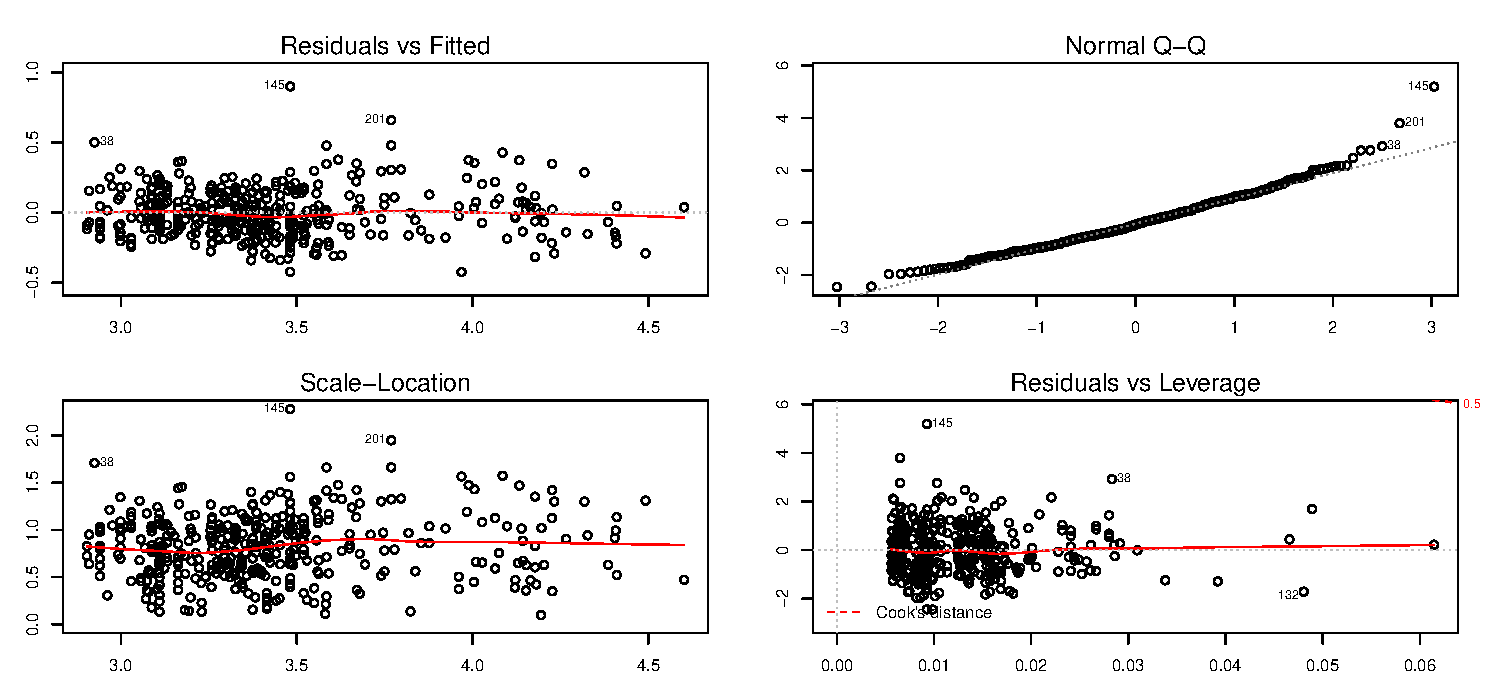
\includegraphics[width=0.9\linewidth]{figures/unnamed-chunk-5-1} \end{center}

\textbf{* Residuals vs Fitted:}\\
Dette plot viser om residualerne har non-lineær mønstre. Hvis
residualerne er indenfor den samme spredning som den horisontale linje,
så er det et tegn på, at der ikke er non-lineær forhold i modellen.\\
Vi kan på vores figur se, at residualerne er spredt omkring den
horisontale linje. Det tyder altså på, at der ikke er non-lineær
tendenser i modellen. Havde vores røde linje haft form som en parabel,
ville det tyde på der var non-lineær forhold i modellen.\\

\textbf{* Normal Q-Q:}\\
Dette plot viser os om residualerne er normalfordelte. Hvis residualerne
er normalfordelte, vil residualerne følge den prikkede streg.\\
Vi kan se i vores figur at alle residualerne ligger tæt på den prikkede
linje, som tyder på at vores residualer er normalfordelte.\\
\newpage

\textbf{* Scale-Location:}\\
Dette plot bruger vi til at checke vores antagelse om lige stor varians
for vores residualer (homoskedasticitet). Hvis de standarliserede
residualer er spredt lige omkring vores predictors(estimator), så
opfylder modellen antagelsen om homoskedasticitet.\\
Vi kan i vores figur se, at residualernes spredning er tæt på den samme
op til omkring 3.5, hvor det ser ud som om der sker en ændring i
variansen for vores residualer. Dette kan indikere, at der er en grad af
heteroskedacitet i vores model.\\

\textbf{* Residuals vs Leverage:}\\
Vi bruger dette plot til at se om vores model har signifikante outliers.
Nogengange kan outliers have en stor effekt på resultatet, der kommer ud
af regressionen. Vi bruger ''Cooks distance'' til at afgøre om vores
residualer har signifikante outlisers. Det kan ses øverst til
højre/right at ''Cooks distance'' starter der for værdien 0.5.\\
Vi kan i vores figur se at vores residualer ikke har outliers, der har
en signifikant påvirkning på vores resultat. Det kan vi se fordi alle
residualerne er indenfor ''Cooks distance''. \newpage

\hypertarget{test-for-heteroskedasticitet-vha.-breusch-pagan-testen-og-specialudgaven-af-white-testet.}{%
\subsection{Test for heteroskedasticitet vha. Breusch-Pagan-testen og
specialudgaven af
White-testet.}\label{test-for-heteroskedasticitet-vha.-breusch-pagan-testen-og-specialudgaven-af-white-testet.}}

\leavevmode

Det vi vil i denne opgave er at teste MLR5, altså om homoskedasticitet
er opfyldt i modellen. Dette er yderligere beskrevet i:
\hyperref[sec:SLR]{Appendix 2 - SLR og MLR antagelser}.\\
~\\
Hvis vi har heteroskedasticity i vores model, vil det påvirke variansen
for vores estimator og dermed gøre vores estimator bias. Det betyder at
vores OLS ikke længere kan beskrives som værende Best Linear Unbiased
Estimate(\hyperref[sec:BLUE]{BLUE}) fordi MLR 5 ikke er opfyldt..\\
~\\
Det vi gør, er at teste for, om en af de uafhænige variable har en
effekt for variansen af fejlleddet. Vores varians burde være konstant,
og burde derfor ikke være afhængige af vores uafhængige variable. Det
kan vi opskrive på hypoteseform:\\
\[H_0:Var[u|x_1,...,x_k]=\sigma^2\] Omskrives:
\[H_0:[u^2|x_1,...,x_k]=\sigma^2\] Dette kan vi fordi:
\[Var(u)=E[u-E(u)]^2\text{ og antagelsen om}\ E(u)=0\] Vi er nu i stand
til at teste for heteroskedasticity ved at bruge \(u^2\), fordi den
forventede værdi af \(u^2\) burde give os variansen af fejlleddet. Da vi
ikke kender \(u^2\) for hele vores population, må vi istedet bruge den
estimerede \(u^2\). \newline 
\hyperref[sec:BP-test]{Breusch-Pagan-testen} udføres:

\begin{Shaded}
\begin{Highlighting}[]
\KeywordTok{bptest}\NormalTok{(model) }\CommentTok{# DF = 4 er vores højreside variable af modellen}
\CommentTok{## }
\CommentTok{##  studentized Breusch-Pagan test}
\CommentTok{## }
\CommentTok{## data:  model}
\CommentTok{## BP = 12.105, df = 4, p-value = 0.01659}
\end{Highlighting}
\end{Shaded}

Der kan også laves en manuel test:

\begin{Shaded}
\begin{Highlighting}[]
\NormalTok{u <-}\StringTok{ }\KeywordTok{residuals}\NormalTok{(model)}
\NormalTok{u2 <-}\StringTok{ }\NormalTok{u}\OperatorTok{^}\DecValTok{2}
\NormalTok{umodel <-}\StringTok{ }\KeywordTok{lm}\NormalTok{(u2 }\OperatorTok{~}\StringTok{ }\NormalTok{educ }\OperatorTok{+}\StringTok{ }\NormalTok{lsalbeginn }\OperatorTok{+}\StringTok{ }\NormalTok{male }\OperatorTok{+}\StringTok{ }\NormalTok{minority, }\DataTypeTok{data =}\NormalTok{ data1)}
\KeywordTok{summary}\NormalTok{(umodel)}
\CommentTok{## }
\CommentTok{## Call:}
\CommentTok{## lm(formula = u2 ~ educ + lsalbeginn + male + minority, data = data1)}
\CommentTok{## }
\CommentTok{## Residuals:}
\CommentTok{##      Min       1Q   Median       3Q      Max }
\CommentTok{## -0.04943 -0.02453 -0.01263  0.00845  0.76913 }
\CommentTok{## }
\CommentTok{## Coefficients:}
\CommentTok{##              Estimate Std. Error t value Pr(>|t|)  }
\CommentTok{## (Intercept)  0.009579   0.027300   0.351   0.7259  }
\CommentTok{## educ         0.002966   0.001360   2.182   0.0297 *}
\CommentTok{## lsalbeginn  -0.008181   0.013072  -0.626   0.5318  }
\CommentTok{## male         0.009813   0.007127   1.377   0.1693  }
\CommentTok{## minority    -0.008087   0.007111  -1.137   0.2561  }
\CommentTok{## ---}
\CommentTok{## Signif. codes:  0 '***' 0.001 '**' 0.01 '*' 0.05 '.' 0.1 ' ' 1}
\CommentTok{## }
\CommentTok{## Residual standard error: 0.05702 on 396 degrees of freedom}
\CommentTok{## Multiple R-squared:  0.03019,    Adjusted R-squared:  0.02039 }
\CommentTok{## F-statistic: 3.082 on 4 and 396 DF,  p-value: 0.01614}
\end{Highlighting}
\end{Shaded}

Her kan vi i begge tilfælde se, at p-værdien \textless{} 0.05, og vi kan
derfor forkaste nulhypotesen om, at der er homoskedacitet. Det vil altså
sige, at der er heteroskedacitet, og derfor har fejlleddet(u) en
sammenhæng med de forklarende variable på højresiden af vores model.\\
\newline  \textbf{White-testen}\\
White testen er en statistisk test, som tester om variansen af fejledene
for regressionen. Det er altså en test, der tester for heteroskedasitet.

\begin{Shaded}
\begin{Highlighting}[]
\KeywordTok{bptest}\NormalTok{(model, }\OperatorTok{~}\StringTok{ }\KeywordTok{fitted}\NormalTok{(model) }\OperatorTok{+}\StringTok{ }\KeywordTok{I}\NormalTok{(}\KeywordTok{fitted}\NormalTok{(model)}\OperatorTok{^}\DecValTok{2}\NormalTok{))}
\CommentTok{## }
\CommentTok{##  studentized Breusch-Pagan test}
\CommentTok{## }
\CommentTok{## data:  model}
\CommentTok{## BP = 8.1481, df = 2, p-value = 0.01701}
\end{Highlighting}
\end{Shaded}

Vi kan også med brug af White-testen afvise \(H_0\) på et 5\%
signifikansnivau, da vores p-værdi er \textcolor{blue}{0.017}. Det
betyder altså at vores model har heteroskedasticitet i sig. \newpage

\hypertarget{beregn-robuste-standardfejl-for-modellen-og-sammenlign-med-resultaterne-i-spuxf8rgsmuxe5l-1.}{%
\subsection{Beregn robuste standardfejl for modellen og sammenlign med
resultaterne i spørgsmål
1.}\label{beregn-robuste-standardfejl-for-modellen-og-sammenlign-med-resultaterne-i-spuxf8rgsmuxe5l-1.}}

\leavevmode

Normalt er vi i stand til at udregne variansen for \(\beta_{\hat{j}}\)
ved at bruge formlen:
\[\frac{\sum\limits_{i=1}^{n}(x_i-\bar{x})^2Var(u_i)}{(SST_x)^2}\]
Normalt ville vi bruge antagelsen om, at variansen for fejlleddet er
konstant, og derfor at \(var(u_i)=\sigma^2\). Det betyder, at variansen
ikke ændrer sig, når man går fra én observation til den næste
observation for en enkelt variabel. Så hvis vi ser på indkomst som en
variabel, så ændrer variansen sig ikke, om vi ser på Anders' indkomst
eller Pouls indkomst. Det betyder også at variansen ikke ændrer sig, når
vi går fra en variabel\((x_1)\) til en anden variabel\((x_2)\). Altså,
at variansen ikke ændrer sig fra fx indkomst\((x_1)\) til
formue\((x_2)\).\\
~\\
Problemet opstår dog fordi den første parantes i ligningen nedenfor,
korrelerer med variansen til \(u_i\)(fejlleddet):
\[corr((x_i-\bar{x})|var(u_i))\neq0 \] fejlleddet korrelerer enten fra
observation til observation, eller fra variabel til variabel. Det
betyder, at der er heteroskedasitet.\\
\hspace*{0.333em}Vi gør istedet brug af robust standardfejl, da disse
ikke korrellerer med fejlleddet. Man kan altså få estimationer, selvom
der er hetereoskedasicitet.\\
\[\sqrt{\frac{\sum\limits_{i=1}^{n}\hat{r}_{ij}^2\hat{u}_i^2}{(SSR_j)^2}} \]
\[\text{hvor }\hat{r}_{ij}^2\ \text{er noteringen for den i’ene residual fra regressionen $(x_j)$}\ \text{på alle andre uafhængige variable }\]\\
For at være i stand til at bruge den ligning ovenfor, så er vi nødt til
at være afhængige af \hyperref[sec:lawoflarge]{law of large numbers} og
\hyperref[sec:CLT]{central limit theorem}.

\begin{Shaded}
\begin{Highlighting}[]
\NormalTok{robustmodel <-}\StringTok{ }\KeywordTok{coeftest}\NormalTok{(model, }\DataTypeTok{vcov =} \KeywordTok{vcovHC}\NormalTok{(model, }\DataTypeTok{type =} \StringTok{"HC0"}\NormalTok{))}
\NormalTok{summodel <-}\StringTok{ }\KeywordTok{summary}\NormalTok{(model)}
\NormalTok{std.error <-}\StringTok{ }\KeywordTok{data.frame}\NormalTok{(}\DataTypeTok{Std.error =}\NormalTok{ summodel}\OperatorTok{$}\NormalTok{coefficients[,}\DecValTok{2}\NormalTok{])}
\NormalTok{Robust.std.error <-}\StringTok{ }\KeywordTok{data.frame}\NormalTok{(}\DataTypeTok{Robust.Std.Error =}\NormalTok{ robustmodel[,}\DecValTok{2}\NormalTok{])}
\KeywordTok{cbind}\NormalTok{(std.error, Robust.std.error)}
\CommentTok{##               Std.error Robust.Std.Error}
\CommentTok{## (Intercept) 0.083361423      0.088866810}
\CommentTok{## educ        0.004151627      0.003820617}
\CommentTok{## lsalbeginn  0.039915108      0.042538198}
\CommentTok{## male        0.021761780      0.022393761}
\CommentTok{## minority    0.021712349      0.019441016}
\end{Highlighting}
\end{Shaded}

Her kan vi se, at der er forskel fra std. error fra opgave 1 og de
robuste std. errors.\\

\hypertarget{test-hypotesen-h_0-beta_2-1-mod-alternativet-h_1-beta_2-neq-1.}{%
\subsection{\texorpdfstring{Test hypotesen \(H_0 : \beta_2 = 1\) mod
alternativet
\(H_1 : \beta_2 \neq 1.\)}{Test hypotesen H\_0 : \textbackslash beta\_2 = 1 mod alternativet H\_1 : \textbackslash beta\_2 \textbackslash neq 1.}}\label{test-hypotesen-h_0-beta_2-1-mod-alternativet-h_1-beta_2-neq-1.}}

Her vil vi gerne finde T-statistikken ud fra følgende formel:
\[ t=(\hat{\beta_j}-1)/se(\hat{\beta_j})\] Finder de nødvendige værdier
til at finde T-statistikken og finder derefter T-statistikken

\begin{Shaded}
\begin{Highlighting}[]
\NormalTok{reg=summodel}\OperatorTok{$}\NormalTok{coefficients}
\NormalTok{beta_}\DecValTok{2}\NormalTok{=}\StringTok{ }\NormalTok{reg[}\DecValTok{3}\NormalTok{,}\DecValTok{1}\NormalTok{]}
\NormalTok{se_beta_}\DecValTok{2}\NormalTok{ =}\StringTok{ }\NormalTok{reg[}\DecValTok{3}\NormalTok{,}\DecValTok{2}\NormalTok{]}
\CommentTok{#T-statistikken}
\NormalTok{(beta_}\DecValTok{2-1}\NormalTok{)}\OperatorTok{/}\NormalTok{se_beta_}\DecValTok{2}
\CommentTok{## [1] -4.488569}
\end{Highlighting}
\end{Shaded}

Finder de kritiske værdier for de forskellige siknifikansniveauer:

\begin{Shaded}
\begin{Highlighting}[]
\NormalTok{alpha <-}\StringTok{ }\KeywordTok{c}\NormalTok{(}\FloatTok{0.1}\NormalTok{,}\FloatTok{0.05}\NormalTok{,}\FloatTok{0.01}\NormalTok{)}
\KeywordTok{qt}\NormalTok{(}\DecValTok{1}\OperatorTok{-}\NormalTok{alpha, }\DataTypeTok{df =} \DecValTok{396}\NormalTok{)}
\CommentTok{## [1] 1.283693 1.648711 2.335801}
\end{Highlighting}
\end{Shaded}

Vores aboslutte værdi er 4.488, og vi kan derfor afvise vores \(H_0\)
hypotese om at \(\beta_2 = 1\) på et 1\% siknifikans niveau, fordi vores
absolutte t-værdi er større end den kritiske værdi på 2.335, og
\(\beta_2\) må derfor være forskellige fra 1. \newpage

\hypertarget{test-hypotesen-h_0-beta_3-beta_4-0.}{%
\subsection{\texorpdfstring{Test hypotesen
\(H_0 : \beta_3 = \beta_4 = 0\).}{Test hypotesen H\_0 : \textbackslash beta\_3 = \textbackslash beta\_4 = 0.}}\label{test-hypotesen-h_0-beta_3-beta_4-0.}}

\textcolor{blue}{Dette er en joint nul hypotese}

Vi har tidligere i opgave 1.3 vist, at der er heteroskedacitet i
modellen, og vi vil derfor kun teste hypotesen på en måde, hvor der er
heteroskedacitet i modellen.\\
~\\
Vi vil bruge wald-testen for at teste om vores \(\beta_3\) og
\(\beta_4\) er lig 0. Vi bruger wald-test fordi den tester om
variablerne er signifikante. Der bliver lavet to modeller, i den første
ingår alle variablene i modellen. I den anden, er de to dummy variabler
ikke med.

\begin{Shaded}
\begin{Highlighting}[]
\KeywordTok{waldtest}\NormalTok{(model, }\DataTypeTok{vcov=}\KeywordTok{vcovHC}\NormalTok{(model, }\DataTypeTok{type =} \StringTok{"HC0"}\NormalTok{), }\DataTypeTok{terms=}\NormalTok{(}\DecValTok{3}\OperatorTok{:}\DecValTok{4}\NormalTok{))}
\CommentTok{## Wald test}
\CommentTok{## }
\CommentTok{## Model 1: lsalary ~ educ + lsalbeginn + male + minority}
\CommentTok{## Model 2: lsalary ~ educ + lsalbeginn}
\CommentTok{##   Res.Df Df      F Pr(>F)}
\CommentTok{## 1    396                 }
\CommentTok{## 2    398 -2 1.7072 0.1827}
\end{Highlighting}
\end{Shaded}

Vi kan ikke på et 5\% siknifikansniveau afvise, at disse to dummy
variable er siknifikante for modellen, da p værdien er større end 0.05.
\textcolor{blue}{Her kunne vi også have brugt Linearhypothesis i R til at udregne det.}\\
\textbf{\textit{Hvis modellen havde været med homoskedacitet istedet for heteroskedacitet skulle vi have lavet en regression uden $\beta_3$ og $\beta_4$ og kunne derefter have fundet p-værdien ved hjælp af F-værdien. }}
\newpage

\hypertarget{estimer-modellen-vha.-fgls-og-kommenter-puxe5-resultaterne.}{%
\subsection{Estimer modellen vha. FGLS og kommenter på
resultaterne.}\label{estimer-modellen-vha.-fgls-og-kommenter-puxe5-resultaterne.}}

\leavevmode

Vi vil i denne opgave lave Feasible GLS(FGLS), fordi vi som udgangspunkt
har en funktion \(h(x)\), som vi ikke kender, men vil prøve at opstille
og estimere. Dette gøres, da vi gerne vil fjerne heteroskedasitet i
modellen. Til det vil vi bruge en formel hvor variansen for fejlleddet
ikke er konstant. Det betyder at felledet bliver påvirket af vores x, og
det kan vi opskrives på formen:
\[ var(u|x)=\sigma^2exp(\delta_0+\delta_1x_1+\delta_2x_2+....\delta_kx_k) \]
Da vi ikke ved hvordan x påvirker variansen på fejlleddet kan vi bruge
delen, der omhandler heteroskedasicitet til at estimere \(\hat{h_i}\).
Grunden til dette er, fordi vi ved at hetereoskedasicitet påvirker
variansen \[ var(u|x)=\sigma^2h(x)\] og det derfor er funktionen for
\(h(x)\) vi ønsker at kende.\\

Vi kender ikke vore deltaværdier, så de estimeres fra vores
stikprøvedata, og vi kan derefter fjerne hetereoskedasicitet. Vi finder
deltaerne ved:
\[ u^2=\sigma^2exp(\delta_0+\delta_1x_1+\delta_2x_2+....\delta_kx_k)v\]
Log tages på begge sider
\[ log(u^2)=\delta_0+\delta_1x_1+\delta_2x_2+....\delta_kx_k + e\]\\
Vi vil nu i R finde vores fitted værdier, som noteres \(\hat{g}_i\), da
\(\hat{h_i} = exp(\hat{g_i})\), altså et estimat af h. og lave FGLS
modellen \newpage

\begin{Shaded}
\begin{Highlighting}[]
\NormalTok{logu2 <-}\StringTok{ }\KeywordTok{log}\NormalTok{(}\KeywordTok{resid}\NormalTok{(model)}\OperatorTok{^}\DecValTok{2}\NormalTok{) }\CommentTok{# Finder logged residualer i anden. }
\NormalTok{varreg<-}\StringTok{ }\KeywordTok{lm}\NormalTok{(logu2}\OperatorTok{~}\NormalTok{educ }\OperatorTok{+}\StringTok{ }\NormalTok{lsalbeginn }\OperatorTok{+}\StringTok{ }\NormalTok{male }\OperatorTok{+}\StringTok{ }\NormalTok{minority, }\DataTypeTok{data=}\NormalTok{data1) }\CommentTok{# Regressionsvariansen }
\NormalTok{w <-}\StringTok{ }\KeywordTok{exp}\NormalTok{(}\KeywordTok{fitted}\NormalTok{(varreg)) }\CommentTok{# Her finder vi vægten som vi skal bruge i vores FGLSmodel}
\NormalTok{FGLSmodel <-}\StringTok{ }\KeywordTok{lm}\NormalTok{(lsalary }\OperatorTok{~}\StringTok{ }\NormalTok{educ }\OperatorTok{+}\StringTok{ }\NormalTok{lsalbeginn }\OperatorTok{+}\StringTok{ }\NormalTok{male }\OperatorTok{+}\StringTok{ }\NormalTok{minority, }\DataTypeTok{data=}\NormalTok{data1, }\DataTypeTok{weight =} \DecValTok{1}\OperatorTok{/}\NormalTok{w)}
\NormalTok{FGLSmodel_sum <-}\StringTok{ }\KeywordTok{summary}\NormalTok{(FGLSmodel)}
\KeywordTok{screenreg}\NormalTok{(}\KeywordTok{list}\NormalTok{(}\DataTypeTok{OLS =}\NormalTok{ model, }\DataTypeTok{FGLS =}\NormalTok{ FGLSmodel_sum), }\DataTypeTok{digits =} \DecValTok{4}\NormalTok{)}
\CommentTok{## }
\CommentTok{## =======================================}
\CommentTok{##              OLS           FGLS        }
\CommentTok{## ---------------------------------------}
\CommentTok{## (Intercept)    0.8560 ***    0.8609 ***}
\CommentTok{##               (0.0834)      (0.0851)   }
\CommentTok{## educ           0.0223 ***    0.0203 ***}
\CommentTok{##               (0.0042)      (0.0039)   }
\CommentTok{## lsalbeginn     0.8208 ***    0.8274 ***}
\CommentTok{##               (0.0399)      (0.0397)   }
\CommentTok{## male           0.0289        0.0331    }
\CommentTok{##               (0.0218)      (0.0212)   }
\CommentTok{## minority      -0.0307       -0.0275    }
\CommentTok{##               (0.0217)      (0.0196)   }
\CommentTok{## ---------------------------------------}
\CommentTok{## R^2            0.7953        0.7863    }
\CommentTok{## Adj. R^2       0.7932        0.7842    }
\CommentTok{## Num. obs.    401           401         }
\CommentTok{## RMSE                         1.8276    }
\CommentTok{## =======================================}
\CommentTok{## *** p < 0.001; ** p < 0.01; * p < 0.05}
\end{Highlighting}
\end{Shaded}

Her ses det, at estimaterne er stort set uændret, men standard
errors(paranteserne) er forskellige fra den originale. Dette betyder, at
vi ikke har været i stand til at fjerne al hetereoskedasiciteten i
modellen.\\
\newpage

\hypertarget{har-fgls-estimationen-taget-huxf8jde-for-al-heteroskedasticiteten}{%
\subsection{Har FGLS estimationen taget højde for al
heteroskedasticiteten?}\label{har-fgls-estimationen-taget-huxf8jde-for-al-heteroskedasticiteten}}

\leavevmode

Hvis vi ikke er sikre på at FGLS estimationen har været i stand til
identificere al heteroskedasiteten, kan vi finde de robuste standard
fejl efter FGLS.

\begin{Shaded}
\begin{Highlighting}[]
\NormalTok{FGLS_Robust <-}\StringTok{ }\KeywordTok{coeftest}\NormalTok{(FGLSmodel, }\DataTypeTok{vcov =} \KeywordTok{vcovHC}\NormalTok{(FGLSmodel, }\DataTypeTok{type =} \StringTok{"HC0"}\NormalTok{))}

\KeywordTok{screenreg}\NormalTok{(}\KeywordTok{list}\NormalTok{(}\DataTypeTok{FGLS =}\NormalTok{ FGLSmodel_sum, }\DataTypeTok{Robust_FGLS =}\NormalTok{ FGLS_Robust), }\DataTypeTok{digits =} \DecValTok{4}\NormalTok{)}
\CommentTok{## }
\CommentTok{## ======================================}
\CommentTok{##              FGLS          Robust_FGLS}
\CommentTok{## --------------------------------------}
\CommentTok{## (Intercept)    0.8609 ***   0.8609 ***}
\CommentTok{##               (0.0851)     (0.0910)   }
\CommentTok{## educ           0.0203 ***   0.0203 ***}
\CommentTok{##               (0.0039)     (0.0038)   }
\CommentTok{## lsalbeginn     0.8274 ***   0.8274 ***}
\CommentTok{##               (0.0397)     (0.0433)   }
\CommentTok{## male           0.0331       0.0331    }
\CommentTok{##               (0.0212)     (0.0220)   }
\CommentTok{## minority      -0.0275      -0.0275    }
\CommentTok{##               (0.0196)     (0.0188)   }
\CommentTok{## --------------------------------------}
\CommentTok{## R^2            0.7863                 }
\CommentTok{## Adj. R^2       0.7842                 }
\CommentTok{## Num. obs.    401                      }
\CommentTok{## RMSE           1.8276                 }
\CommentTok{## ======================================}
\CommentTok{## *** p < 0.001; ** p < 0.01; * p < 0.05}
\end{Highlighting}
\end{Shaded}

Vi kan se at modellen ikke var i stand til at fjerne al
heteroskedasticiteten, fordi at standardafvigelserne har ændret sig. Ses
i paranteserne.

\newpage

\includepdf[pages=1,pagecommand=\section{Eksamensopgave 2}, offset=0 -1cm]{opgave2}

\hypertarget{estimer-de-to-modeller-vha.-ols.-kommenter-puxe5-outputtet-sammenlign-og-fortolk-resultaterne.}{%
\subsection{Estimer de to modeller vha. OLS. Kommenter på outputtet,
sammenlign og fortolk
resultaterne.}\label{estimer-de-to-modeller-vha.-ols.-kommenter-puxe5-outputtet-sammenlign-og-fortolk-resultaterne.}}

\leavevmode

Opstiller modellen vha OLS., som vi har udledt i
\hyperref[sec:OLS]{Appendix 1 - OLS}:
\[salary = \beta_0+\beta_1educ+\beta_2salbegin+\beta_3male+\beta_4minority \tag{1}\]
\[ log(salary)=\beta_0+\beta_1educ+\beta_2log(salbegin)+\beta_3male+\beta_4minority+u \tag{2} \]

Her tager vi også udgangspunkt i de 5 MLR antagelser beskrevet i
\hyperref[sec:SLR]{Appendix 2 - SLR og MLR antagelser}.\\
\newline Estimeres ved hjælp af R:

Vi opstiller først \textbf{model 1}, som er en level-level model. Det er
det fordi, at der ikke er taget log af noget, og man bruger det rene
data.

\begin{Shaded}
\begin{Highlighting}[]
\NormalTok{model1 <-}\StringTok{ }\KeywordTok{lm}\NormalTok{(salary }\OperatorTok{~}\StringTok{ }\NormalTok{educ }\OperatorTok{+}\StringTok{ }\NormalTok{salbegin }\OperatorTok{+}\StringTok{ }\NormalTok{male }\OperatorTok{+}\StringTok{ }\NormalTok{minority)}
\KeywordTok{summary}\NormalTok{(model1)}
\CommentTok{## }
\CommentTok{## Call:}
\CommentTok{## lm(formula = salary ~ educ + salbegin + male + minority)}
\CommentTok{## }
\CommentTok{## Residuals:}
\CommentTok{##     Min      1Q  Median      3Q     Max }
\CommentTok{## -28.470  -4.128  -0.705   2.888  48.718 }
\CommentTok{## }
\CommentTok{## Coefficients:}
\CommentTok{##             Estimate Std. Error t value Pr(>|t|)    }
\CommentTok{## (Intercept) -6.93228    1.85539  -3.736 0.000211 ***}
\CommentTok{## educ         0.99327    0.16674   5.957 5.22e-09 ***}
\CommentTok{## salbegin     1.60816    0.06408  25.097  < 2e-16 ***}
\CommentTok{## male         1.83088    0.85713   2.136 0.033220 *  }
\CommentTok{## minority    -1.72539    0.92056  -1.874 0.061547 .  }
\CommentTok{## ---}
\CommentTok{## Signif. codes:  0 '***' 0.001 '**' 0.01 '*' 0.05 '.' 0.1 ' ' 1}
\CommentTok{## }
\CommentTok{## Residual standard error: 7.875 on 445 degrees of freedom}
\CommentTok{## Multiple R-squared:  0.7962, Adjusted R-squared:  0.7944 }
\CommentTok{## F-statistic: 434.7 on 4 and 445 DF,  p-value: < 2.2e-16}
\end{Highlighting}
\end{Shaded}

\textbf{Educ(uddannelse)}\\
Her kan vi se på estimatet at vi har en positiv sammenhæng mellem
uddannelse og salary(årsløn). Resultatet er statistisk signifikant da vi
kan se vi har en meget lav p-værdi, og en meget høj t-værdi. Det betyder
at en øgning i uddannelse på 1 vil øge årslønne med 0.99.\\
\newpage \textbf{Salbegin(startløn)}\\
Vi kan se på estimatet at der en positiv sammenhæng mellem startlønne og
salary(årsløn). Resultater er også signifikant fordi vi har en meget lav
p-værdi, og en meget høj t-værdi. Det vil sige at hvis vi øger
startlønnen med 1(målt i 1000 US dollars), så vil årslønne stige med
1.6(mål i 1000 US dollars).\\

\textbf{Male(mand)}\\
Dette er en dummy variable som tager værdien 1 hvis der er tale om en
mand, og tager værdien 0 hvis der ikke er tale om en mand. Vi kan se at
der er en positiv sammenhæng, men dette resultat er ikke lige så
signifikant som uddannelse og startløn.\\

\textbf{Minority(minoritet)}\\
Dette er en dummy variable som tager værdien 1 hvis der er tale om en
fra en minoritetsgruppe, og værdien 0 der ikke er tale om en der
tilhøjrer en minoritet. Vi kan se der er en negativ sammenhæng mellem at
tilhøjrer en minoritetsgruppe, og så hvilken årsløn man får. Vi kan se
at resultatet ikke er signifikant på et 5\% signifikansniveau.\\

\textbf{Generelt om model 1}\\
For at beskrive styrken i modellen kan vi kigge på \(AdjR^2\). I dette
tilfælde er den 0.79. Dette er højt for økonomisk data, og betyder at
højre siden af regressionen kan forklare venstre-siden relativt godt.
Det betyder dog ikke at der nødvendigvis er en kausalitet.\\

\textbf{Model2} er en log-log model. Her er kravet at venstresiden er
log og minimum én variabel på højre side også er log.

\begin{Shaded}
\begin{Highlighting}[]
\NormalTok{model2 <-}\StringTok{ }\KeywordTok{lm}\NormalTok{(lsalary }\OperatorTok{~}\StringTok{ }\NormalTok{educ }\OperatorTok{+}\StringTok{ }\NormalTok{lsalbegin }\OperatorTok{+}\StringTok{ }\NormalTok{male }\OperatorTok{+}\StringTok{ }\NormalTok{minority)}
\KeywordTok{summary}\NormalTok{(model2)}
\CommentTok{## }
\CommentTok{## Call:}
\CommentTok{## lm(formula = lsalary ~ educ + lsalbegin + male + minority)}
\CommentTok{## }
\CommentTok{## Residuals:}
\CommentTok{##      Min       1Q   Median       3Q      Max }
\CommentTok{## -0.45488 -0.11663 -0.00496  0.11201  0.87115 }
\CommentTok{## }
\CommentTok{## Coefficients:}
\CommentTok{##              Estimate Std. Error t value Pr(>|t|)    }
\CommentTok{## (Intercept)  0.849130   0.077094  11.014  < 2e-16 ***}
\CommentTok{## educ         0.023578   0.003993   5.905 7.01e-09 ***}
\CommentTok{## lsalbegin    0.820725   0.037051  22.151  < 2e-16 ***}
\CommentTok{## male         0.045474   0.020774   2.189   0.0291 *  }
\CommentTok{## minority    -0.041856   0.021057  -1.988   0.0474 *  }
\CommentTok{## ---}
\CommentTok{## Signif. codes:  0 '***' 0.001 '**' 0.01 '*' 0.05 '.' 0.1 ' ' 1}
\CommentTok{## }
\CommentTok{## Residual standard error: 0.1786 on 445 degrees of freedom}
\CommentTok{## Multiple R-squared:  0.8051, Adjusted R-squared:  0.8034 }
\CommentTok{## F-statistic: 459.6 on 4 and 445 DF,  p-value: < 2.2e-16}
\end{Highlighting}
\end{Shaded}

\textbf{Educ(uddannelse)}\\
Vi kan se der er tale om en positiv sammenhæng mellem uddannelse og
log-salary. Dette er et statistisk signifikant resultat, og det kan vi
se fordi vi har en meget lav p-værdi og meget høj t-værdi. Det betyder
at hvis uddannelse stiger med 1 år, så vil årslønnen stige med 2.3\%.
\newline

\textbf{Lsalbegin(logaritmen til startslønnen)}\\
Vi kan se at der er tale om en positiv sammenhæng mellem logaritmen til
startslønnen, og logartimen til årslønnen. Det er et signifikant
resultat, og det kan vi fordi vi har en lav p-værdi og en høj t-værdi.\\

\textbf{Male(mand)}\\
Dette er en dummy variable som tager værdien 1 hvis der er tale om en
mand, og tager værdien 0 hvis der ikke er tale om en mand. Vi kan se at
der er en positiv sammenhæng, men dette resultat er ikke lige så
signifikant som uddannelse og startløn.\\

\textbf{Minority(minoritet)}\\
Dette er en dummy variable som tager værdien 1 hvis der er tale om en
fra en minoritetsgruppe, og værdien 0 der ikke er tale om en der
tilhøjrer en minoritet. Vi kan se der er en negativ sammenhæng mellem at
tilhøjrer en minoritetsgruppe, og så hvilken årsløn man får.\\

\textbf{Generelt om model 2}\\
Vi kan på model 2 se at der er en stærk forklaringsgrad mellem
højre-side variablerne og venstre-side variablerne, og det kan vi se på
\(AdjR^2\).\\

\textbf{Sammenligning af modeller:}\\
Forskellen på disse modeller er måden de bliver opstillet på. Den ene
bliver opstillet som en level-level model, og den anden bliver opstillet
som en log-log model. Måden man tolker dem på er forskellige, fordi når
man tolker på noget, der er logget, så kigger man på procentvise
ændringer. Hvor hvis de ikke er logget, kigger man på de tilhøjrende
værdier. ~Grunden til, at man gerne vil logge nogle variable er fordi,
man gerne vil prøve at skabe en mere linæer sammenhæng mellem variablene
ved at fjerne de ikke-linæere elementer blandt variablerne. Det sker ved
hjælp af, at når man logger noget, så bliver værdierne automatisk
mindre, og man kommer derfor tættere på den linæere trend, og
spredningen bliver derfor mindre. Begge modeller er stærke ifølge deres
\(AdjR^2\),\\
\newpage

\textbf{Hvornår giver det mening at tage log til en variabel?}\\
Hvis vi har en variable der enten er meget left-skewed, eller
right-skewed, så vil det at tage den naturlige logaritme gøre variablen
mere normalfordelt. Det skyldes, at vi ved at log til en variable i en
regression gør, at vi i stedet ser på procentvise ændringer. Det gælder
både for log-level, level-log og log-log modeller.

\hypertarget{udfuxf8r-grafisk-modelkontrol-af-de-to-modeller.-hvilken-model-vil-du-foretruxe6kke}{%
\subsection{Udfør grafisk modelkontrol af de to modeller. Hvilken model
vil du
foretrække?}\label{udfuxf8r-grafisk-modelkontrol-af-de-to-modeller.-hvilken-model-vil-du-foretruxe6kke}}

\leavevmode

\textbf{Residuals vs Fitted:}\\
Dette plot viser om residualerne har non-lineær mønstre. Hvis
residualerne er indenfor den samme spredning som den horisontale linje,
så er det et tegn på, at der ikke er non-lineær forhold i modellen.

\begin{Shaded}
\begin{Highlighting}[]
\KeywordTok{par}\NormalTok{(}\DataTypeTok{mfrow=}\KeywordTok{c}\NormalTok{(}\DecValTok{2}\NormalTok{,}\DecValTok{1}\NormalTok{),}\DataTypeTok{mar=}\KeywordTok{c}\NormalTok{(}\DecValTok{2}\NormalTok{,}\DecValTok{3}\NormalTok{,}\DecValTok{3}\NormalTok{,}\DecValTok{2}\NormalTok{),}\DataTypeTok{cex=}\FloatTok{0.7}\NormalTok{)}
\KeywordTok{plot}\NormalTok{(model1, }\DataTypeTok{which =} \KeywordTok{c}\NormalTok{(}\DecValTok{1}\NormalTok{,}\DecValTok{1}\NormalTok{))}
\KeywordTok{plot}\NormalTok{(model2, }\DataTypeTok{which =} \KeywordTok{c}\NormalTok{(}\DecValTok{1}\NormalTok{,}\DecValTok{1}\NormalTok{))}
\end{Highlighting}
\end{Shaded}

\begin{center}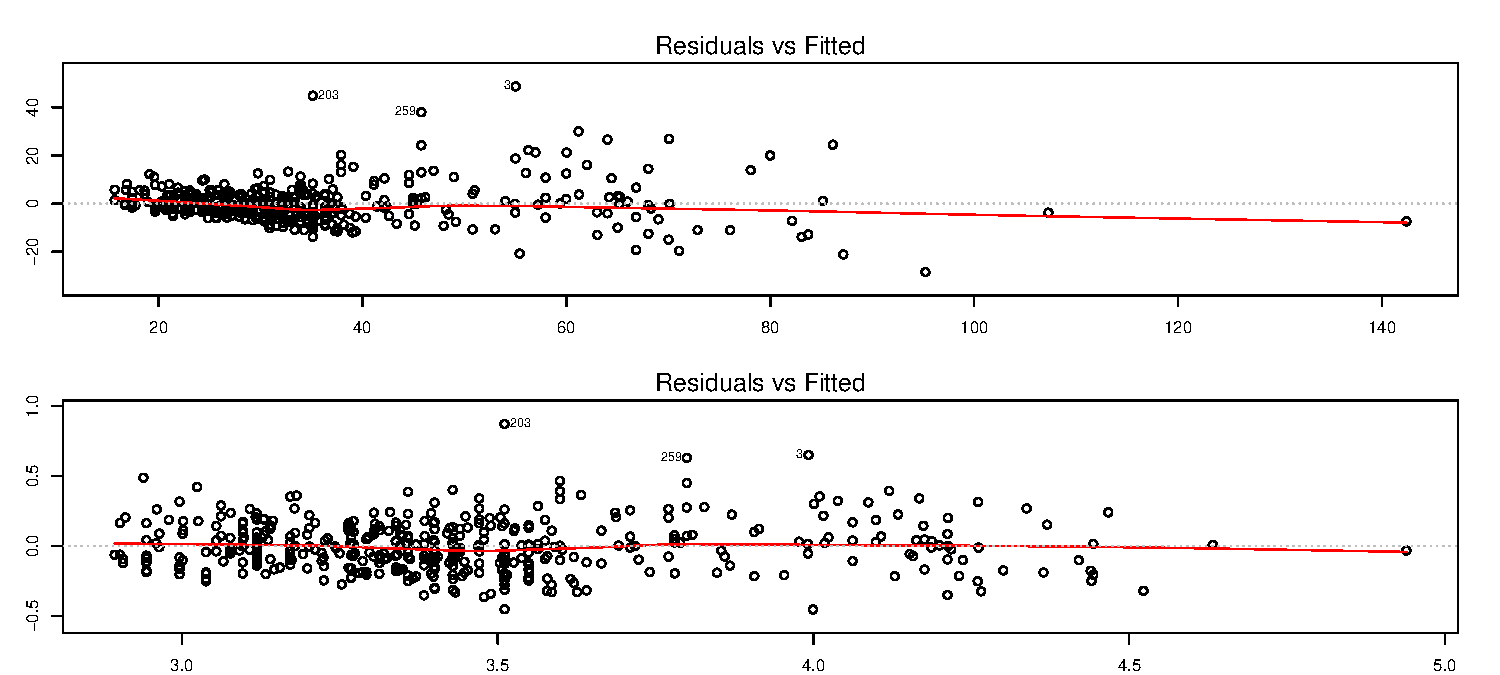
\includegraphics[width=0.9\linewidth]{figures/unnamed-chunk-18-1} \end{center}

I model 1(den øverste) kan vi se, at residualernes spredning er lige
stor omkring den vandrette linje. Dette kunne tyde på, at sammenhængen
er linæer. Vi kan dog også se, at den i slutningen er en smule faldende,
men dette skyldes formentlig er der ikke er særlig mange residualer.\\
I model 2(den nederste) kan vi se stort set det samme. Spredningen er
dog lidt større på residualerne, men der er stadig en linæer trend.\\
\newpage \textbf{Normal Q-Q }\\
Dette plot viser os om residualerne er normalfordelte. Hvis residualerne
er normalfordelte, vil residualerne følge den prikkede streg.

\begin{Shaded}
\begin{Highlighting}[]
\KeywordTok{par}\NormalTok{(}\DataTypeTok{mfrow=}\KeywordTok{c}\NormalTok{(}\DecValTok{2}\NormalTok{,}\DecValTok{1}\NormalTok{),}\DataTypeTok{mar=}\KeywordTok{c}\NormalTok{(}\DecValTok{2}\NormalTok{,}\DecValTok{3}\NormalTok{,}\DecValTok{3}\NormalTok{,}\DecValTok{2}\NormalTok{),}\DataTypeTok{cex=}\FloatTok{0.7}\NormalTok{)}
\KeywordTok{plot}\NormalTok{(model1, }\DataTypeTok{which =} \KeywordTok{c}\NormalTok{(}\DecValTok{2}\NormalTok{,}\DecValTok{2}\NormalTok{))}
\KeywordTok{plot}\NormalTok{(model2, }\DataTypeTok{which =} \KeywordTok{c}\NormalTok{(}\DecValTok{2}\NormalTok{,}\DecValTok{2}\NormalTok{))}
\end{Highlighting}
\end{Shaded}

\begin{center}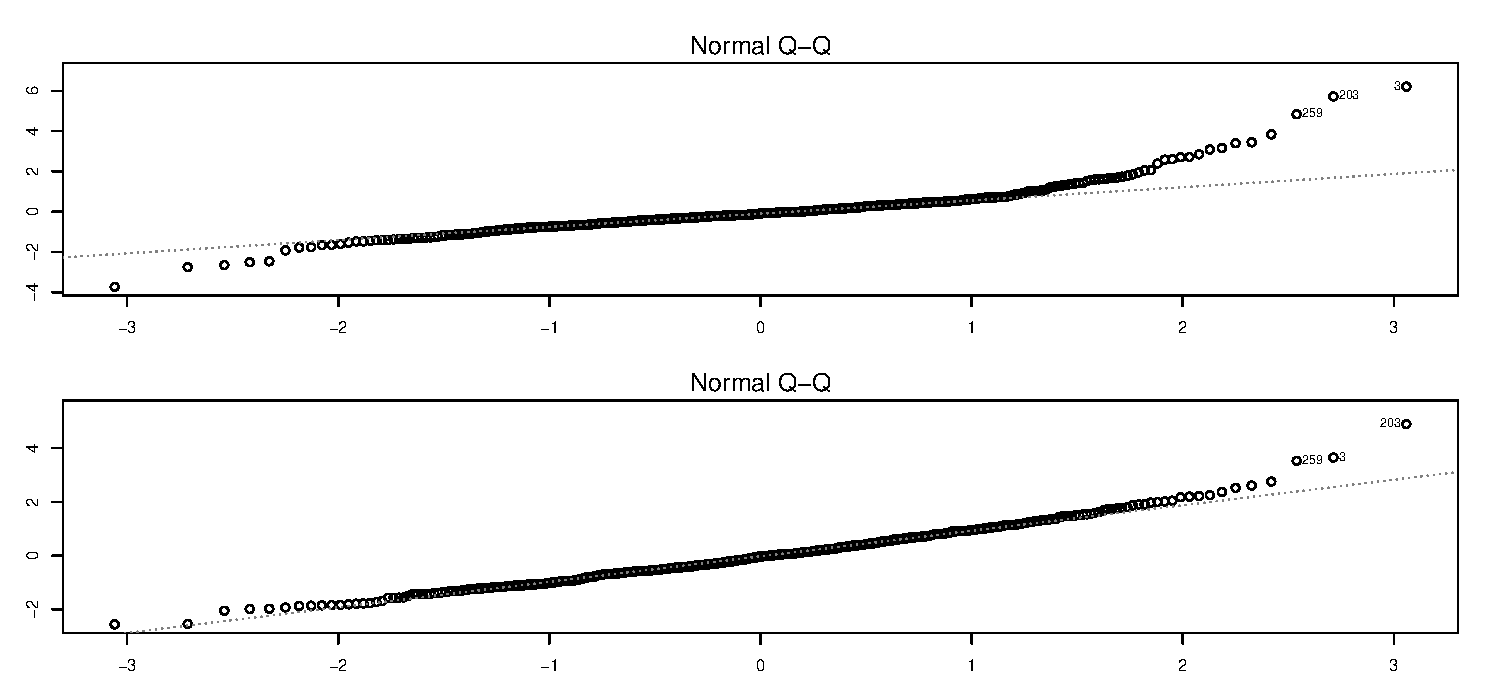
\includegraphics[width=0.9\linewidth]{figures/unnamed-chunk-19-1} \end{center}

I begge tilfølde kan vi se, at de er normalfordelte. Dette er de fordi
de bevæger sig langs den stiblede linje med få outliers. \newpage

\textbf{Scale-location}\\
Dette plot bruger vi til at checke vores antagelse om lige stor varians
for vores residualer (homoskedasticitet). Hvis de standarliserede
residualer er spredt lige omkring vores predictors(estimator), så
opfylder modellen antagelsen om homoskedasticitet.

\begin{Shaded}
\begin{Highlighting}[]
\KeywordTok{par}\NormalTok{(}\DataTypeTok{mfrow=}\KeywordTok{c}\NormalTok{(}\DecValTok{2}\NormalTok{,}\DecValTok{1}\NormalTok{),}\DataTypeTok{mar=}\KeywordTok{c}\NormalTok{(}\DecValTok{2}\NormalTok{,}\DecValTok{3}\NormalTok{,}\DecValTok{3}\NormalTok{,}\DecValTok{2}\NormalTok{),}\DataTypeTok{cex=}\FloatTok{0.7}\NormalTok{)}
\KeywordTok{plot}\NormalTok{(model1, }\DataTypeTok{which =} \KeywordTok{c}\NormalTok{(}\DecValTok{3}\NormalTok{,}\DecValTok{3}\NormalTok{))}
\KeywordTok{plot}\NormalTok{(model2, }\DataTypeTok{which =} \KeywordTok{c}\NormalTok{(}\DecValTok{3}\NormalTok{,}\DecValTok{3}\NormalTok{))}
\end{Highlighting}
\end{Shaded}

\begin{center}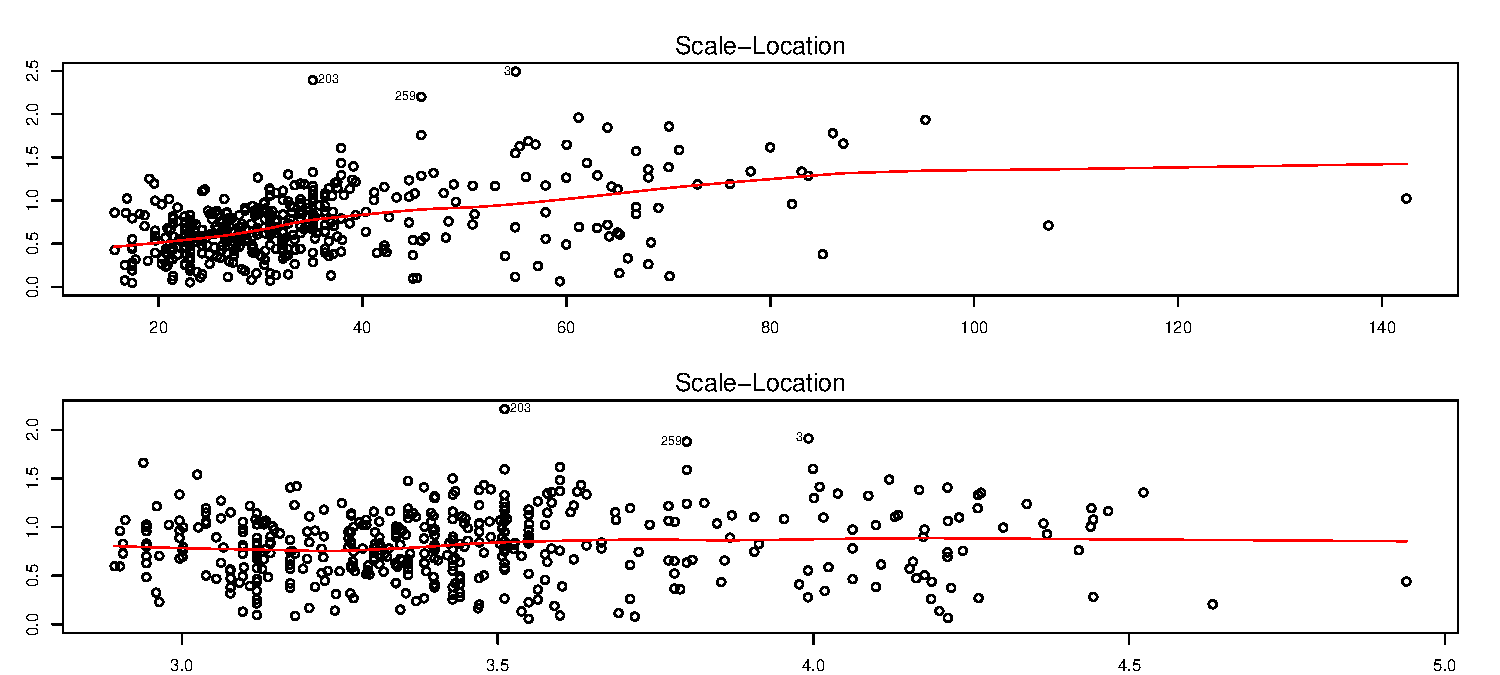
\includegraphics[width=0.9\linewidth]{figures/unnamed-chunk-20-1} \end{center}

I model 1(Den øverste) kan vi se, at residualerne er mere samlede end i
model 2(den nederste). Derudover så kan vi også se, at hældningen på den
røde linje ændrer sig. Dette kunne antyde heteroskedacitet.\\
I model 2(Den nederste) ændrer hældningen sig ikke. Dette tyder på
homoskedacitet.\\
- Der kunne også anvendes lmtest eller white-test for at undersøge
dette. Dette gør vi dog ikke. \newpage

\textbf{Residuals vs leverage}\\
Vi bruger dette plot til at se om vores model har signifikante outliers.
Nogengange kan outliers have en stor effekt på resultatet, der kommer ud
af regressionen. Vi bruger ''Cooks distance'' til at afgøre om vores
residualer har signifikante outlisers.

\begin{Shaded}
\begin{Highlighting}[]
\KeywordTok{par}\NormalTok{(}\DataTypeTok{mfrow=}\KeywordTok{c}\NormalTok{(}\DecValTok{2}\NormalTok{,}\DecValTok{1}\NormalTok{),}\DataTypeTok{mar=}\KeywordTok{c}\NormalTok{(}\DecValTok{2}\NormalTok{,}\DecValTok{3}\NormalTok{,}\DecValTok{3}\NormalTok{,}\DecValTok{2}\NormalTok{),}\DataTypeTok{cex=}\FloatTok{0.7}\NormalTok{)}
\KeywordTok{plot}\NormalTok{(model1, }\DataTypeTok{which =} \KeywordTok{c}\NormalTok{(}\DecValTok{5}\NormalTok{,}\DecValTok{5}\NormalTok{))}
\KeywordTok{plot}\NormalTok{(model2, }\DataTypeTok{which =} \KeywordTok{c}\NormalTok{(}\DecValTok{5}\NormalTok{,}\DecValTok{5}\NormalTok{))}
\end{Highlighting}
\end{Shaded}

\begin{center}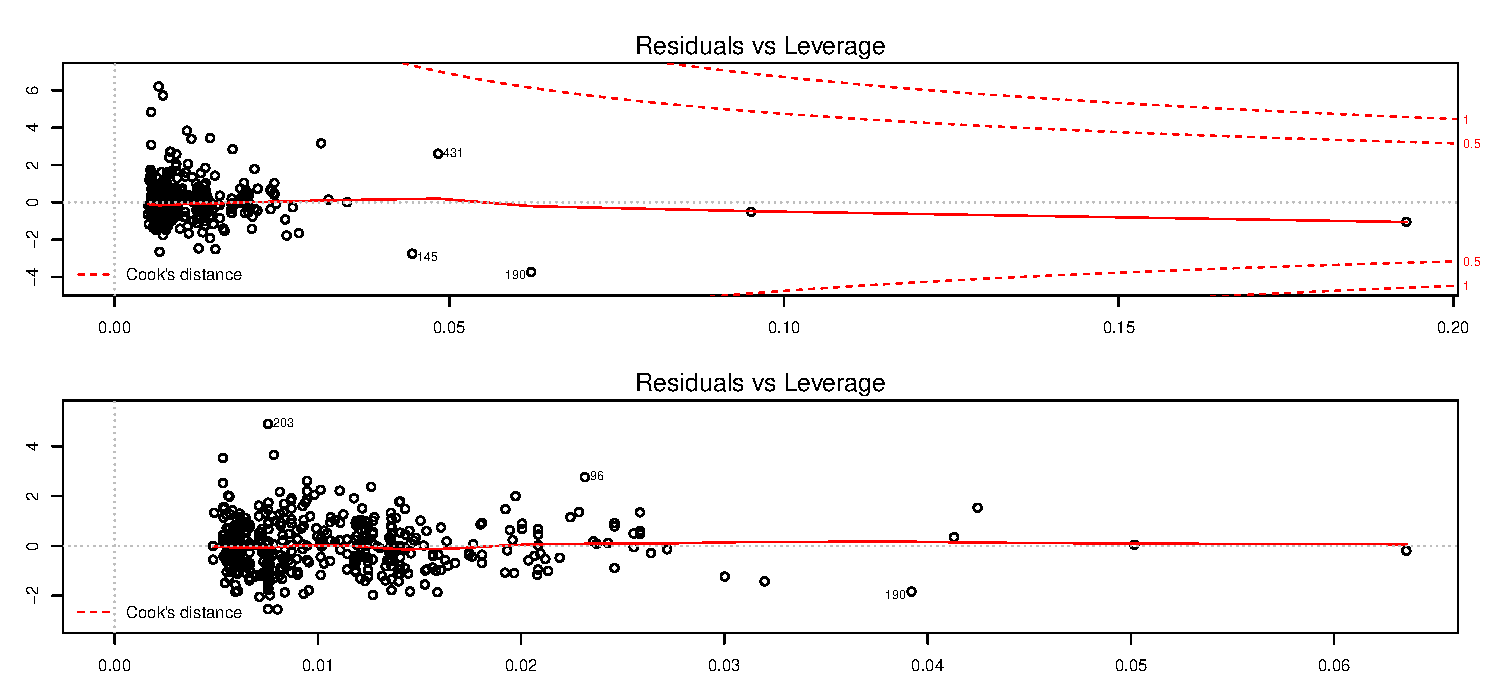
\includegraphics[width=0.9\linewidth]{figures/unnamed-chunk-21-1} \end{center}

I model 1(Den øverste) kan vi se, at vi, at der er nogle observationer,
der er tæt på at komme udenfor ``Cooks distance''. Dette betyder, at det
er outliers, der kan have en stor påvirkning på vores datasæt og
estimator. Man kan derfor overveje at fjerne dem. Det gør vi dog ikke,
fordi de ikke er helt udenfor distancen.\\
I model 2(Den nederste) er der ikke særlig mange outliers, og dem der
er, er ikke store nok til at have indflydelse på vores estimator.\\
~\\
\textbf{Hvilken model vil vi foretrække?}\\
Hvis vi tager udgangspunkt i vores grafer, så kan vi se en tendens for
model 2, der gør den mere favorabel end model 1.\\
Model 2 har mere linære linjer i Residuals vs Fitted og Scale-location.
Dette tyder på en mere normalfordelt model med få outliers.\\
Derudover kan vi også se i Residuals vs leverage, at model 2 er længere
væk fra ``Cook's distance'', hvilket betyder, at der ikke er nogle
siknifikante outliers. Heller ikke nogle der er tæt på, at være
siknifikante. ~ I normal Q-Q kan vi se, at model 2 er mere
normalfordelt. \newpage

\hypertarget{undersuxf8g-om-de-to-modeller-er-misspecificerede-vha.-reset-testet.}{%
\subsection{Undersøg om de to modeller er misspecificerede vha.
RESET-testet.}\label{undersuxf8g-om-de-to-modeller-er-misspecificerede-vha.-reset-testet.}}

\leavevmode

Reset testen bruges til at undersøge om der er nogle non-linæere
sammenhænge i en linæer model. Dette gøres ved hjælp af en F-test på en
Joint nulhypotese, hvor nulhypotesen er: \[ H_0:\gamma_1=\gamma_2=0\]

Det at have misspecifikation i sin regressionsmodel, er et alvorligt
problem. Hvis vi har misspecifikation betyder det, at vi har en fejl i
vores model. Helt konkret så betyder det, at vores regressionsmodel ikke
har taget højde for alting(det er umuligt at tage højde for alting).
Hvis vi er ude for misspecifikation, så kan vores estimator og fejlled
være biased.\\
Der er tre former for model misspecifikation:\\
~\\
- Den første er hvis vi udelader relevante variabler, og dett kan skabe
model misspecifikation.\\
- Den anden er hvis vi medtager irrelevante variabler i
regressionensligningen.\\
- Den tredje er hvis vi ikke opskriver regressionsmodellen på den rette
funktionelle form, som kunne være ikke at have sat en variable i anden
eller lignende.\\

Den form for model misspecifikation vi vil teste for er den 3 variant,
som omhandler funktionel form.

Først tester vi for \textbf{model1:}

\begin{Shaded}
\begin{Highlighting}[]
\KeywordTok{resettest}\NormalTok{(model1)}
\CommentTok{## }
\CommentTok{##  RESET test}
\CommentTok{## }
\CommentTok{## data:  model1}
\CommentTok{## RESET = 2.5756, df1 = 2, df2 = 443, p-value = 0.07725}
\end{Highlighting}
\end{Shaded}

Vi får en p-værdi på 0.07 og vi kan derfor på et 10\% signifikansnivau
afvise \(H_0\). Det betyder at der er misspecifikation i vores
regression.\\
Så tester vi for \textbf{model2:}

\begin{Shaded}
\begin{Highlighting}[]
\KeywordTok{resettest}\NormalTok{(model2)}
\CommentTok{## }
\CommentTok{##  RESET test}
\CommentTok{## }
\CommentTok{## data:  model2}
\CommentTok{## RESET = 2.6338, df1 = 2, df2 = 443, p-value = 0.07293}
\end{Highlighting}
\end{Shaded}

Vi får i vores model en p-værdi på 0.07, og vi kan derfor på et 10\%
signifikansnivau afvise \(H_0\). Det betyder at der er misspecifikantion
i vores regression. \newpage

\hypertarget{forklar-hvorfor-det-kunne-vuxe6re-relevant-at-medtage-educ2-som-forklarende-variabel-i-de-to-modeller.-estimer-de-to-modeller-igen-hvor-educ2-inkluderes-med-tilhuxf8jrende-koefficient-beta_5-kommenter-kort-puxe5-outputtet-og-udfuxf8r-reset-testet-igen.}{%
\subsection{\texorpdfstring{Forklar hvorfor det kunne være relevant at
medtage \(educ^2\) som forklarende variabel i de to modeller. Estimer de
to modeller igen hvor \(educ^2\) inkluderes ( med tilhøjrende
koefficient \(\beta_5\) ), kommenter kort på outputtet og udfør
RESET-testet
igen.}{Forklar hvorfor det kunne være relevant at medtage educ\^{}2 som forklarende variabel i de to modeller. Estimer de to modeller igen hvor educ\^{}2 inkluderes ( med tilhøjrende koefficient \textbackslash beta\_5 ), kommenter kort på outputtet og udfør RESET-testet igen.}}\label{forklar-hvorfor-det-kunne-vuxe6re-relevant-at-medtage-educ2-som-forklarende-variabel-i-de-to-modeller.-estimer-de-to-modeller-igen-hvor-educ2-inkluderes-med-tilhuxf8jrende-koefficient-beta_5-kommenter-kort-puxe5-outputtet-og-udfuxf8r-reset-testet-igen.}}

\leavevmode

\textcolor{blue}{vi har i tidligere opgave fundet misspecifikation i modellen, hvor en af problemerne kan være, at den står på den forkerte funktionelle form, og derfor kunne det være interessant at prøve at tage $educ^2$ med for at ændre den funktionelle form.}\\
Hvis vi medtager \(educ^2\) får vi en ny regressionsmodel:
\[ salary = \beta_0+\beta_1educ+\beta_2salbegin+\beta_3male+\beta_4minority+\beta_5educ^2+u \tag{1} \]
\[ log(salary)=\beta_0+\beta_1educ+\beta_2log(salbegin)+\beta_3male+\beta_4minority+\beta_5educ^2+u \tag{2} \]
Relevansen for at medtage \(educ^2\) er hvis vi mistænker at forholdet
mellem educ og vores afhængige variabel y, ikke er lineært.\\
Argumentet for dette kunne være aftagende marginalprodukt på uddannelse,
så at første år har en positiv effekt på den årlige indkomst. Det samme
har de efterfølgende år op til et vist punkt, hvorefter effekten bliver
negativ.

\textbf{$educ^2$ estimeres og reset-testen udføres igen}

\begin{Shaded}
\begin{Highlighting}[]
\NormalTok{model1}\FloatTok{.4}\NormalTok{ <-}\StringTok{ }\KeywordTok{lm}\NormalTok{(salary }\OperatorTok{~}\StringTok{ }\NormalTok{educ }\OperatorTok{+}\StringTok{ }\NormalTok{salbegin }\OperatorTok{+}\StringTok{ }\NormalTok{male }\OperatorTok{+}
\StringTok{                      }\NormalTok{minority }\OperatorTok{+}\StringTok{ }\NormalTok{educ2)}

\NormalTok{model2}\FloatTok{.4}\NormalTok{ <-}\StringTok{ }\KeywordTok{lm}\NormalTok{(lsalary }\OperatorTok{~}\StringTok{ }\NormalTok{educ }\OperatorTok{+}\StringTok{  }\NormalTok{lsalbegin }\OperatorTok{+}\StringTok{ }\NormalTok{male }\OperatorTok{+}\StringTok{ }
\StringTok{                 }\NormalTok{minority }\OperatorTok{+}\StringTok{ }\NormalTok{educ2)}

\KeywordTok{summary}\NormalTok{(model1}\FloatTok{.4}\NormalTok{)}
\CommentTok{## }
\CommentTok{## Call:}
\CommentTok{## lm(formula = salary ~ educ + salbegin + male + minority + educ2)}
\CommentTok{## }
\CommentTok{## Residuals:}
\CommentTok{##     Min      1Q  Median      3Q     Max }
\CommentTok{## -24.264  -4.042  -0.870   2.891  49.720 }
\CommentTok{## }
\CommentTok{## Coefficients:}
\CommentTok{##             Estimate Std. Error t value Pr(>|t|)    }
\CommentTok{## (Intercept) 14.60237    6.78940   2.151  0.03203 *  }
\CommentTok{## educ        -2.30474    1.01458  -2.272  0.02359 *  }
\CommentTok{## salbegin     1.47994    0.07438  19.897  < 2e-16 ***}
\CommentTok{## male         1.78553    0.84791   2.106  0.03578 *  }
\CommentTok{## minority    -1.61496    0.91115  -1.772  0.07701 .  }
\CommentTok{## educ2        0.13205    0.04008   3.294  0.00107 ** }
\CommentTok{## ---}
\CommentTok{## Signif. codes:  0 '***' 0.001 '**' 0.01 '*' 0.05 '.' 0.1 ' ' 1}
\CommentTok{## }
\CommentTok{## Residual standard error: 7.79 on 444 degrees of freedom}
\CommentTok{## Multiple R-squared:  0.8011, Adjusted R-squared:  0.7989 }
\CommentTok{## F-statistic: 357.7 on 5 and 444 DF,  p-value: < 2.2e-16}
\KeywordTok{summary}\NormalTok{(model2}\FloatTok{.4}\NormalTok{)}
\CommentTok{## }
\CommentTok{## Call:}
\CommentTok{## lm(formula = lsalary ~ educ + lsalbegin + male + minority + educ2)}
\CommentTok{## }
\CommentTok{## Residuals:}
\CommentTok{##      Min       1Q   Median       3Q      Max }
\CommentTok{## -0.44932 -0.11908 -0.00702  0.11246  0.87400 }
\CommentTok{## }
\CommentTok{## Coefficients:}
\CommentTok{##               Estimate Std. Error t value Pr(>|t|)    }
\CommentTok{## (Intercept)  1.1754018  0.2073494   5.669 2.59e-08 ***}
\CommentTok{## educ        -0.0147950  0.0229937  -0.643   0.5203    }
\CommentTok{## lsalbegin    0.7825191  0.0433061  18.069  < 2e-16 ***}
\CommentTok{## male         0.0483029  0.0207975   2.323   0.0207 *  }
\CommentTok{## minority    -0.0416353  0.0210129  -1.981   0.0482 *  }
\CommentTok{## educ2        0.0015510  0.0009153   1.694   0.0909 .  }
\CommentTok{## ---}
\CommentTok{## Signif. codes:  0 '***' 0.001 '**' 0.01 '*' 0.05 '.' 0.1 ' ' 1}
\CommentTok{## }
\CommentTok{## Residual standard error: 0.1782 on 444 degrees of freedom}
\CommentTok{## Multiple R-squared:  0.8064, Adjusted R-squared:  0.8042 }
\CommentTok{## F-statistic: 369.8 on 5 and 444 DF,  p-value: < 2.2e-16}
\KeywordTok{resettest}\NormalTok{(model1}\FloatTok{.4}\NormalTok{)}
\CommentTok{## }
\CommentTok{##  RESET test}
\CommentTok{## }
\CommentTok{## data:  model1.4}
\CommentTok{## RESET = 1.8771, df1 = 2, df2 = 442, p-value = 0.1543}
\KeywordTok{resettest}\NormalTok{(model2}\FloatTok{.4}\NormalTok{)}
\CommentTok{## }
\CommentTok{##  RESET test}
\CommentTok{## }
\CommentTok{## data:  model2.4}
\CommentTok{## RESET = 1.8884, df1 = 2, df2 = 442, p-value = 0.1525}
\end{Highlighting}
\end{Shaded}

Hvis vi kigger på de to modeller kan vi nu se, at siknifikansniveauerne
ikke er de samme som
tidligere.~\textcolor{blue}{P-værdien er blevet større, og vi kan derfor ikke forkaste $H_0$ fra tidligere opgave. Det vil altså nu sige, at der ikke er misspecifikation i modellen. $educ^2$ har altså styrket vores model}\\
Derudover kan vi se, at fordi vi har brugt \(educ^2\) som \(\beta_5\),
så har estimatoren ændret sig til positivt fortegn. Dette indikerer, at
der er et minimumspunkt i education, hvilket er naturligt, fordi vi får
en parabel, når vi sætter ting i anden.

\hypertarget{test-hypotesen-h_0-beta_1-beta_5-0-i-begge-modeller-fra-spuxf8rgsmuxe5l-4.}{%
\subsection{\texorpdfstring{Test hypotesen
\(H_0 : \beta_1 = \beta_5 = 0\) i begge modeller (fra spørgsmål
4).}{Test hypotesen H\_0 : \textbackslash beta\_1 = \textbackslash beta\_5 = 0 i begge modeller (fra spørgsmål 4).}}\label{test-hypotesen-h_0-beta_1-beta_5-0-i-begge-modeller-fra-spuxf8rgsmuxe5l-4.}}

\leavevmode

Her vil vi gerne teste for om \(\beta_1educ\) og \(\beta_5educ^2\) er
siknifikante for modellen, altså en ``Joint null hypothesis''. Til dette
kan vi bruge F-testen, hvis man vil gøre det manuelt\\
Først opstilles en nulhypotese: \[ H_0:\beta_1=\beta_5=0\] F-testen
opstilles:
\[F=\frac{R_{ur}^2-R_r^2}{1-R_{ur}^2}*\frac{n-k-1}{q},\ hvor\ q=df_r-df_{ur} \]
Hvis man ikke vil anvende F-testen manuelt, kan man istedet gøre det
direkte i R ved hjælp af Linearhypothesis kommandoen.\\
\textbf{Model 1}

\begin{Shaded}
\begin{Highlighting}[]

\NormalTok{h0_a =}\StringTok{ }\KeywordTok{c}\NormalTok{(}\StringTok{"educ=0"}\NormalTok{,}\StringTok{"educ2=0"}\NormalTok{)}
\KeywordTok{linearHypothesis}\NormalTok{(model1}\FloatTok{.4}\NormalTok{, h0_a)}
\CommentTok{## Linear hypothesis test}
\CommentTok{## }
\CommentTok{## Hypothesis:}
\CommentTok{## educ = 0}
\CommentTok{## educ2 = 0}
\CommentTok{## }
\CommentTok{## Model 1: restricted model}
\CommentTok{## Model 2: salary ~ educ + salbegin + male + minority + educ2}
\CommentTok{## }
\CommentTok{##   Res.Df   RSS Df Sum of Sq      F   Pr(>F)    }
\CommentTok{## 1    446 29801                                 }
\CommentTok{## 2    444 26941  2    2859.5 23.563 1.88e-10 ***}
\CommentTok{## ---}
\CommentTok{## Signif. codes:  0 '***' 0.001 '**' 0.01 '*' 0.05 '.' 0.1 ' ' 1}
\end{Highlighting}
\end{Shaded}

Ved en P-værdi under 0.01 kan vi forkaste på et 1\% siknifikans niveau,
og vi kan derfor afvise nulhypotesen. Dette betyder at uddannelse er
siknifikant i modellen. Så vi kan ikke undlade uddannelse uden det ville
påvirke modellen.\\
\textbf{Model 2}

\begin{Shaded}
\begin{Highlighting}[]
\NormalTok{h0_b =}\StringTok{ }\KeywordTok{c}\NormalTok{(}\StringTok{"educ=0"}\NormalTok{,}\StringTok{"educ2=0"}\NormalTok{)}
\KeywordTok{linearHypothesis}\NormalTok{(model2}\FloatTok{.4}\NormalTok{, h0_b)}
\CommentTok{## Linear hypothesis test}
\CommentTok{## }
\CommentTok{## Hypothesis:}
\CommentTok{## educ = 0}
\CommentTok{## educ2 = 0}
\CommentTok{## }
\CommentTok{## Model 1: restricted model}
\CommentTok{## Model 2: lsalary ~ educ + lsalbegin + male + minority + educ2}
\CommentTok{## }
\CommentTok{##   Res.Df    RSS Df Sum of Sq      F    Pr(>F)    }
\CommentTok{## 1    446 15.306                                  }
\CommentTok{## 2    444 14.102  2    1.2033 18.942 1.275e-08 ***}
\CommentTok{## ---}
\CommentTok{## Signif. codes:  0 '***' 0.001 '**' 0.01 '*' 0.05 '.' 0.1 ' ' 1}
\end{Highlighting}
\end{Shaded}

Ved en P-værdi under 0.01 kan vi forkaste på et 1\% siknifikans niveau,
og vi kan derfor afvise nulhypotesen. Dette betyder at uddannelse er
siknifikant i modellen. Så vi kan ikke undlade uddannelse uden det ville
påvirke modellen.\\

\hypertarget{kunne-der-vuxe6re-problemer-med-muxe5lefejl-i-de-to-modeller-i-hvilke-tilfuxe6lde-vil-det-udguxf8re-et-problem}{%
\subsection{Kunne der være problemer med målefejl i de to modeller? I
hvilke tilfælde vil det udgøre et
problem?}\label{kunne-der-vuxe6re-problemer-med-muxe5lefejl-i-de-to-modeller-i-hvilke-tilfuxe6lde-vil-det-udguxf8re-et-problem}}

\leavevmode

I en regression vil der altid være chance for målefejl. Det skyldes, at
vi er begrænset af hvor mange uafhængige variable, vi kan tage med i
modellen, og der derfor selvfølgelig være variable, der bliver
udeladt.\\

\textcolor{blue}{Teoretisk kan målefejl forklares både for den afhængige variabel og den uafhængige:}\\
\textbf{Afhængig variabel(y)}\\
\textcolor{blue}{Målefejlen bliver noteret $e_0$, hvor der er nogle antagelser specifikt for den afhængige variabel: }
\[ E(u)=E(e_o)=0\] \[ Cov(u,e_0)=0\] \[ Cov(e_o,x)=0\]
\textcolor{blue}{Hvis disse antagelser er overholdt, vil OLS estimaterne være unbiased og konsistente. Hvis de bliver brudt vil estimaterne for intercept være biased, dog er hældningen på regressionen uændret. Er der målefejl i modellen vil variansen for OLS estimaterne også blive større. \
Dette kan løses ved at løse målefejlen, men det kan være rigtig svært at løse, udover at indhente bedre data.}\\
~\\
\textbf{Et eksempel på en målefejl i den afhængige variabel: Årlig opsparing i familien:}\\
\textcolor{blue}{Her kan der opstå en målefejl, fordi familier har en tendens til at indrappotere deres opsparing forkert. Dette giver os en større varians i fejlleddet}\\
\newpage

\textbf{Uafhængig variabel(x)}\\
Hvis målefejlen er forbundet med en uafhængige variable, så er problemet
af en anden karakter. Vi vil forklare dette ved, at opstille en
teoretisk model, hvor målefejlen er forbundet med \(x_1\), som vi
noterer \(x^*_1\).\\
\textcolor{blue}{SLR1 til SLR4 antages at være overholdt. Dette betyder, at ved estimation af modellen fåes unbiased og konsistente estimatorer.\
Problemet opstår, fordi vi ikke kender $x^*_1$ og bliver derfor nødt til at bruge $x_1$ til estimere. \
Et eksempel for $x^*_1$ kunne være den faktiske indkomst, hvor $x_1$ er den rapporterede indkomst. Så der er altså forskel mellem disse to. Det kunne fx. være}
``sorte penge''.\\
Modellen opstilles: \[ y=\beta_0+\beta_1x^\ast_1 +u\]
\textcolor{blue}{Vi skal bruge et nyt fejlled, fordi der er en forskel mellem vores $x$ variabler, der ikke indgår i modellen, og derfor antages at være en del af fejlleddet. Dette nye fejlled er et fejlled for populationen:
\[ e_1 =x_1-x^\ast_1\] 
isolerer $x_1^*$
\[\ x^\ast_1=x_1-e_1 \]
og indsætte denne i den oprindelige model:
\[ y=\beta_0+\beta_1(x_1-e_1) +u\]
Ganger ind i parantesen: 
\[ y=\beta_0+\beta_1x_1-\beta_1e_1 +u \]
Omskriver: 
\[y=\beta_0+\beta_1x_1+u-\beta_1e_1 \]
\[hvor\ E(u)=E(e)=0 \]}\\
Nu er der to scenarier:\\
\textbf{Scenarie 1:}\\
Hvis \(e_1\) er ukorreleret med \(x_1\) gælder det at:
\[ Cov(x_1,e_1)=0\] og det gælder derfor \[ Cov(x^\ast_1,e_1)\neq0 \]
\textcolor{blue}{Dette vil skabe en større varians, men estimatorne vil stadigvæk være unbiased og konsistente. Så dette er ikke et problem for modellen, fordi vi har $x_1$ med i modellen, og denne korrelerer ikke med fejlleddet.}\\
~\\
\textbf{Scenarie 2:}\\
Hvis det omvendte gør sig gældende så vil det gælde at:
\[ Cov(x^\ast_1,e_1)=0 \] og det må derfor gælde at
\[ Cov(x_1,e_1)\neq0\]
\textcolor{blue}{Nu er der opstået et problem. Nu korrelerer vores $x_1$ med fejlleddet i modellen. Dette skaber altså bias i vores estimatorer. }
\newpage

\includepdf[pages=1,pagecommand=\section{Eksamensopgave 3}, offset=0 -1cm]{opgave3}

\hypertarget{estimer-modellen-vha.-ols-og-kommenter-puxe5-resultaterne.}{%
\subsection{Estimer modellen vha. OLS og kommenter på
resultaterne.}\label{estimer-modellen-vha.-ols-og-kommenter-puxe5-resultaterne.}}

\leavevmode

Her skal vi estimere en model ved hjælp af OLS. OLS er udledt i
\hyperref[sec:OLS]{Appendix 1 - OLS} ~ Modellen opstilles:
\[log(earnings)\beta_0+\beta_1s+\beta_2wexp+\beta_3male+\beta_4ethblack+\beta_5ethhisp+u\]
Modellen opstilles i R:

\begin{Shaded}
\begin{Highlighting}[]
\NormalTok{model_}\DecValTok{3}\NormalTok{_opg_}\DecValTok{1}\NormalTok{ <-}\StringTok{ }\KeywordTok{lm}\NormalTok{(}\KeywordTok{log}\NormalTok{(data3}\OperatorTok{$}\NormalTok{earnings) }\OperatorTok{~}\StringTok{ }\NormalTok{data3}\OperatorTok{$}\NormalTok{s }\OperatorTok{+}\StringTok{ }\NormalTok{data3}\OperatorTok{$}\NormalTok{wexp }\OperatorTok{+}\StringTok{ }
\StringTok{                      }\NormalTok{data3}\OperatorTok{$}\NormalTok{male }\OperatorTok{+}\StringTok{ }\NormalTok{data3}\OperatorTok{$}\NormalTok{ethblack }\OperatorTok{+}\StringTok{ }\NormalTok{data3}\OperatorTok{$}\NormalTok{ethhisp)}
\KeywordTok{summary}\NormalTok{(model_}\DecValTok{3}\NormalTok{_opg_}\DecValTok{1}\NormalTok{)}
\CommentTok{## }
\CommentTok{## Call:}
\CommentTok{## lm(formula = log(data3$earnings) ~ data3$s + data3$wexp + data3$male + }
\CommentTok{##     data3$ethblack + data3$ethhisp)}
\CommentTok{## }
\CommentTok{## Residuals:}
\CommentTok{##      Min       1Q   Median       3Q      Max }
\CommentTok{## -2.07585 -0.28006 -0.00145  0.30775  1.98441 }
\CommentTok{## }
\CommentTok{## Coefficients:}
\CommentTok{##                 Estimate Std. Error t value Pr(>|t|)    }
\CommentTok{## (Intercept)     0.396226   0.173508   2.284  0.02280 *  }
\CommentTok{## data3$s         0.124220   0.009451  13.143  < 2e-16 ***}
\CommentTok{## data3$wexp      0.033882   0.005046   6.715 4.99e-11 ***}
\CommentTok{## data3$male      0.293449   0.045803   6.407 3.36e-10 ***}
\CommentTok{## data3$ethblack -0.195670   0.071255  -2.746  0.00624 ** }
\CommentTok{## data3$ethhisp  -0.097406   0.100342  -0.971  0.33213    }
\CommentTok{## ---}
\CommentTok{## Signif. codes:  0 '***' 0.001 '**' 0.01 '*' 0.05 '.' 0.1 ' ' 1}
\CommentTok{## }
\CommentTok{## Residual standard error: 0.5103 on 514 degrees of freedom}
\CommentTok{## Multiple R-squared:  0.3539, Adjusted R-squared:  0.3476 }
\CommentTok{## F-statistic: 56.32 on 5 and 514 DF,  p-value: < 2.2e-16}
\end{Highlighting}
\end{Shaded}

Her kigger vi på en log-level model. Før vi kan tolke på resultaterne,
skal vi lave nogle antagelser:\\
- Vi antager Gaus markov antagelserne holder. - Disse er beskrevet i
\hyperref[sec:SLR]{Appendix 2 - SLR og MLR antagelser}.\\
- Vi antager også at vores resultater er statistisk signifikante med
undtagelse af hispanic etniciteten.\\
~\\
Nu kan vi kommentere på vores resultater og her skal vi tolke på, hvad
der sker med, hvis vi ændrer højre-variablen med 1. Så lad os sige, at
uddannelse(s) stiger med 1 år, så kan vi se på vores estimater, at
lønnen stiger med 12,4\%. Hvis erhvervserfaring(exp) stiger med 1 år, så
stiger lønnen med 3,3\%. vi kan også se, at hvis man er mand så stiger
lønnen med 29,3\%. Lønnen falder med -19,5\% hvis man er sort. Lønnen
skulle falde med 9,7\%, hvis man er hispanic. Dette resultat er dog ikke
statistik signifikant.

\hypertarget{hvorfor-kunne-vi-vuxe6re-bekymrede-for-at-uddannelse-er-endogen}{%
\subsection{Hvorfor kunne vi være bekymrede for at uddannelse er
endogen?}\label{hvorfor-kunne-vi-vuxe6re-bekymrede-for-at-uddannelse-er-endogen}}

Vi kan være bekymret for om variablen for uddannelse(s) er endogen, og
derfor at den vil korrelere med fejlleddet \[cov(x_1,u)\neq0\] Vi ved at
der kan være flere forskellige grunde til at uddannelse kan være
korreleret til fejlleddet. Den første kan være på grund af vi ikke har
medtaget alle signifikante variable i vores regression (omitted
variables). Den anden kan være målefejl i den uafhængige variable(x).
Den tredje kan være hvis den afhængige variable(y), har en effekt på den
uafhængige variable(x) (two way correlation).\\

Vi kan fra ovenstående konkludere, at det er mest sandsynligt at der er
tale om, at vi lider af ikke at have taget alle relevante variable
med(omitted variables). Det kunne være fordi vi ikke har medtaget en
variabel, der siger noget om evnerne(abilities). Grunden til vi ikke har
denne med kunne være, fordi det er svært at finde en proxy variable for
evner.\\
Det kan beskrives ud fra følgende formler:\\
Den sande model: \[ y=\beta_0+\beta_1x_1+\beta_2x_2+u \tag{1}\] \(x_2\)
udlades \[y=\beta_0+\beta_1x_1+u \tag{2}\] Det betyder, at hvis vi havde
at: \[cov(x_1,x_2)\neq0\] Så ville vores estimat være biased.\\
Når vi undlader \(x_2\) fra vores model, vil effekten bliver absorberet
i fejlleddet. Det betyder, at vi kan have at \(x_1\) er korreleret med
fejlleddet. \[cov(x_1,u)\neq 0\] Dette ville være en overtrædelse af MLR
4 og betyder, at modellen er biased.

\hypertarget{er-siblings-sm-og-sf-brugbare-som-instrumenter}{%
\subsection{Er siblings, sm og sf brugbare som
instrumenter?}\label{er-siblings-sm-og-sf-brugbare-som-instrumenter}}

Variablerne ovenfor kan være brugbare, hvis de korrelerer med personens
uddannelse. Dette kan vi teste ved at lave tre regressioner, hvor vi
sætter uddannelse, som den afhængige variabel. Instrumentvariablerne som
er siblings, sm og sf sætter vi som uafhængige variabler og resten af
regressionsmodellen forbliver uændret.

\begin{Shaded}
\begin{Highlighting}[]
\NormalTok{sib_reg <-}\StringTok{ }\KeywordTok{lm}\NormalTok{(data3}\OperatorTok{$}\NormalTok{s}\OperatorTok{~}\NormalTok{data3}\OperatorTok{$}\NormalTok{wexp}\OperatorTok{+}\NormalTok{data3}\OperatorTok{$}\NormalTok{male}\OperatorTok{+}\NormalTok{data3}\OperatorTok{$}\NormalTok{ethblack}\OperatorTok{+}\NormalTok{data3}\OperatorTok{$}\NormalTok{ethhisp}\OperatorTok{+}\NormalTok{data3}\OperatorTok{$}\NormalTok{siblings)}
\NormalTok{sm_reg <-}\StringTok{ }\KeywordTok{lm}\NormalTok{(data3}\OperatorTok{$}\NormalTok{s}\OperatorTok{~}\NormalTok{data3}\OperatorTok{$}\NormalTok{wexp}\OperatorTok{+}\NormalTok{data3}\OperatorTok{$}\NormalTok{male}\OperatorTok{+}\NormalTok{data3}\OperatorTok{$}\NormalTok{ethblack}\OperatorTok{+}\NormalTok{data3}\OperatorTok{$}\NormalTok{ethhisp}\OperatorTok{+}\NormalTok{data3}\OperatorTok{$}\NormalTok{sm)}
\NormalTok{sf_reg <-}\StringTok{ }\KeywordTok{lm}\NormalTok{(data3}\OperatorTok{$}\NormalTok{s}\OperatorTok{~}\NormalTok{data3}\OperatorTok{$}\NormalTok{wexp}\OperatorTok{+}\NormalTok{data3}\OperatorTok{$}\NormalTok{male}\OperatorTok{+}\NormalTok{data3}\OperatorTok{$}\NormalTok{ethblack}\OperatorTok{+}\NormalTok{data3}\OperatorTok{$}\NormalTok{ethhisp}\OperatorTok{+}\NormalTok{data3}\OperatorTok{$}\NormalTok{sf)}
\KeywordTok{screenreg}\NormalTok{(}\KeywordTok{list}\NormalTok{(}\DataTypeTok{SibReg =}\NormalTok{ sib_reg, }\DataTypeTok{smReg =}\NormalTok{ sm_reg, }\DataTypeTok{sfReg =}\NormalTok{ sf_reg ), }\DataTypeTok{digits =} \DecValTok{5}\NormalTok{)}
\CommentTok{## }
\CommentTok{## ===========================================================}
\CommentTok{##                 SibReg         smReg          sfReg        }
\CommentTok{## -----------------------------------------------------------}
\CommentTok{## (Intercept)      16.74267 ***   11.04228 ***   12.53157 ***}
\CommentTok{##                  (0.42146)      (0.59852)      (0.51517)   }
\CommentTok{## data3$wexp       -0.13046 ***   -0.11495 ***   -0.12304 ***}
\CommentTok{##                  (0.02238)      (0.02082)      (0.02106)   }
\CommentTok{## data3$male        0.02298        0.02571        0.07743    }
\CommentTok{##                  (0.21010)      (0.19445)      (0.19694)   }
\CommentTok{## data3$ethblack   -1.05002 **    -0.87737 **    -0.80045 ** }
\CommentTok{##                  (0.32614)      (0.30074)      (0.30657)   }
\CommentTok{## data3$ethhisp    -0.69045        0.50380        0.04364    }
\CommentTok{##                  (0.46086)      (0.44711)      (0.44257)   }
\CommentTok{## data3$siblings   -0.22961 ***                              }
\CommentTok{##                  (0.04963)                                 }
\CommentTok{## data3$sm                         0.39919 ***               }
\CommentTok{##                                 (0.03846)                  }
\CommentTok{## data3$sf                                        0.27757 ***}
\CommentTok{##                                                (0.02904)   }
\CommentTok{## -----------------------------------------------------------}
\CommentTok{## R^2               0.12052        0.24265        0.22214    }
\CommentTok{## Adj. R^2          0.11196        0.23528        0.21457    }
\CommentTok{## Num. obs.       520            520            520          }
\CommentTok{## ===========================================================}
\CommentTok{## *** p < 0.001; ** p < 0.01; * p < 0.05}
\end{Highlighting}
\end{Shaded}

Her kan vi se, at alle tre variable har en korrelation til uddannelse,
som også er statistisk siknifikant. Det må altså forventes, at disse
variable er brugbare som instrumenter. Dog er det stadigvæk vigtigt at
påpege, at disse ikke må korrelere med fejlleddet(ability), da de i så
fald vil have en kovarrians forskellig fra nul og ikke længere er
uafhængige variable. Dette kan dog ikke testes og må derfor tages i en
diskussion:\\
~\\
\textbf{Siblings}:\\
Det kan ikke umiddelbart antages, at evner og søskende skulle have en
covarians. De må derfor være uafhængige og brugbare som instrumenter.\\
~\\
\textbf{Moderens uddannelse(sm) og faderens uddannelse(sf)}\\
Disse kunne godt være faktorer, der gik ind og havde en påvirkning på
evner, da de i forskellige studier er vist, at folk der kommer fra
veluddannede hjem, som udgangspunkt er bedre stillet end det modsatte.\\
Da dette er tilfældet, er det ikke nødvendigvis uafhængige variabler, og
kan gå ind og korrelerer med evner og bør ikke bruges som instrumenter.
Gør man dette, vil det have stor effekt på resultaterne \newpage

\hypertarget{test-om-uddannelse-er-endogen.}{%
\subsection{Test om uddannelse er
endogen.}\label{test-om-uddannelse-er-endogen.}}

\leavevmode

\textcolor{blue}{Endogenitet kan opstår i en model, hvis vi har en uafhængig variabel i modellen, der er korreleret med fejlleddet. Dette kunne være på grund af, at man mangler en variabel "omitted variable" eller målefejl}\\
Vi antager en regressionsmodel på følgende formel:
\[ y_1 = \beta_0 + \beta_1y_2+\beta_2x_1+\beta_3x_2+u\] Her mistænker vi
\(y_2\) for at være endogen, hvor vi har vores instrumenter(siblings, sm
og sf) og vil derfor teste for dette.\\
Er \(y_2\) endogen vil der være en kovarians med u, hvilket betyder, at
de er afhængige af hinanden. Dette er ikke optimalt da det skaber bias i
modellen.\\
\textcolor{blue}{For at teste dette, skal vi lave en OLS(som vi har fra tidligere opgaver) og en 2SLS, som vi gør nu:}\\
Vores model opstilles på den reducerede form for \(y_2\) for at kunne
lave en regressionstest senere:
\[ y_2=\pi_0+\pi_1x_1+\pi_2x_2+\pi_3z_1+\pi_4z_2+\pi_5z_3+v\] Hvor
z-værdierne er vores instrumentvariable fra tidligere.\\
~\\
Inden testen antager vi først, at vores instrumentvariable ikke
korrelerer med u, altså \[corr(Z,u)=0\ \text{hvor}\ Z=(z_1,z_2,z_3) \]
Dette betyder også, at \(y_2\) ikke korrelerer med \(u\), hvis vores
fejlled \(v\) ikke korrelerer med \(u\).\\
Det vi ønsker at teste er altså at \(v\) og \(u\) ikke korrelerer med
hinanden. Dog kender vi ikke v, og derfor skal denne estimeres. Det
gøres ved hjælp af vores reducerede ligning ovenfor, hvor vi bruger
estimatet derfra. \(\hat{v}\) indsættes nu i den originale model:
\[ y_1 = \beta_0 + \beta_1y_2+\beta_2x_1+\beta_3x_2+\delta_1\hat{v}+ e\]
\(\delta_1\) er hentet fra udtrykket for u: \(u=\delta_1v+e\), hvor e er
ukorreleret med \(v_2\). Vi kan derfor se, at \(u\) og \(v\) kun er
ukorreleret, hvis \(\delta_1=0\).\\
Ud fra dette kan nulhypotesen opstilles og vi kan udføre vores test:
\[H_0:\delta_1=0\] Hvis vi kan afvise \(H_0\), kan vi konkludere at
\(v\) og \(u\) korrelerer med hinanden og \(y_2\) er endogen.\\
Laves i R:

\begin{Shaded}
\begin{Highlighting}[]
\NormalTok{stage1 <-}\StringTok{ }\KeywordTok{lm}\NormalTok{(data3}\OperatorTok{$}\NormalTok{s }\OperatorTok{~}\StringTok{ }\NormalTok{data3}\OperatorTok{$}\NormalTok{wexp }\OperatorTok{+}\StringTok{ }\NormalTok{data3}\OperatorTok{$}\NormalTok{male }\OperatorTok{+}\StringTok{ }\NormalTok{data3}\OperatorTok{$}\NormalTok{ethblack }\OperatorTok{+}\StringTok{ }\NormalTok{data3}\OperatorTok{$}\NormalTok{ethhisp}
             \OperatorTok{+}\StringTok{ }\NormalTok{data3}\OperatorTok{$}\NormalTok{siblings }\OperatorTok{+}\StringTok{ }\NormalTok{data3}\OperatorTok{$}\NormalTok{sf }\OperatorTok{+}\StringTok{ }\NormalTok{data3}\OperatorTok{$}\NormalTok{sm) }\CommentTok{# Reduceret form for y2.}

\NormalTok{res =}\StringTok{ }\KeywordTok{resid}\NormalTok{(stage1) }\CommentTok{# Residualer}

\CommentTok{# modellen med y1 med v(hat)}
\NormalTok{stage2 <-}\StringTok{ }\KeywordTok{lm}\NormalTok{(}\KeywordTok{log}\NormalTok{(data3}\OperatorTok{$}\NormalTok{earnings) }\OperatorTok{~}\StringTok{ }\NormalTok{data3}\OperatorTok{$}\NormalTok{s }\OperatorTok{+}\StringTok{ }\NormalTok{data3}\OperatorTok{$}\NormalTok{wexp }\OperatorTok{+}\StringTok{ }\NormalTok{data3}\OperatorTok{$}\NormalTok{male}
             \OperatorTok{+}\StringTok{ }\NormalTok{data3}\OperatorTok{$}\NormalTok{ethblack }\OperatorTok{+}\StringTok{ }\NormalTok{data3}\OperatorTok{$}\NormalTok{ethhisp }\OperatorTok{+}\StringTok{ }\NormalTok{res, }\DataTypeTok{data =}\NormalTok{ data3) }
\CommentTok{#Koefficienter}
\KeywordTok{coeftest}\NormalTok{(stage2) }
\CommentTok{## }
\CommentTok{## t test of coefficients:}
\CommentTok{## }
\CommentTok{##                 Estimate Std. Error t value  Pr(>|t|)    }
\CommentTok{## (Intercept)    -0.064700   0.339003 -0.1909   0.84871    }
\CommentTok{## data3$s         0.153036   0.020516  7.4593 3.742e-13 ***}
\CommentTok{## data3$wexp      0.037628   0.005567  6.7591 3.784e-11 ***}
\CommentTok{## data3$male      0.290479   0.045775  6.3458 4.869e-10 ***}
\CommentTok{## data3$ethblack -0.157544   0.075122 -2.0972   0.03647 *  }
\CommentTok{## data3$ethhisp  -0.069476   0.101739 -0.6829   0.49499    }
\CommentTok{## res            -0.036550   0.023106 -1.5818   0.11430    }
\CommentTok{## ---}
\CommentTok{## Signif. codes:  0 '***' 0.001 '**' 0.01 '*' 0.05 '.' 0.1 ' ' 1}
\end{Highlighting}
\end{Shaded}

Man kan også bruge wu-hausman testen, som gør det hele automatisk.
Resultatet skulle være det samme:

\begin{Shaded}
\begin{Highlighting}[]
\NormalTok{test <-}\StringTok{ }\KeywordTok{ivreg}\NormalTok{(}\KeywordTok{log}\NormalTok{(data3}\OperatorTok{$}\NormalTok{earnings) }\OperatorTok{~}\StringTok{ }\NormalTok{data3}\OperatorTok{$}\NormalTok{s }\OperatorTok{+}\StringTok{ }\NormalTok{data3}\OperatorTok{$}\NormalTok{wexp }\OperatorTok{+}\StringTok{ }\NormalTok{data3}\OperatorTok{$}\NormalTok{male}
              \OperatorTok{+}\StringTok{ }\NormalTok{data3}\OperatorTok{$}\NormalTok{ethblack }\OperatorTok{+}\StringTok{ }\NormalTok{data3}\OperatorTok{$}\NormalTok{ethhisp }\OperatorTok{|}\StringTok{ }
\StringTok{                }\NormalTok{data3}\OperatorTok{$}\NormalTok{wexp }\OperatorTok{+}\StringTok{ }\NormalTok{data3}\OperatorTok{$}\NormalTok{male }\OperatorTok{+}\StringTok{ }\NormalTok{data3}\OperatorTok{$}\NormalTok{ethblack }\OperatorTok{+}\StringTok{ }\NormalTok{data3}\OperatorTok{$}\NormalTok{ethhisp}
              \OperatorTok{+}\StringTok{ }\NormalTok{data3}\OperatorTok{$}\NormalTok{siblings }\OperatorTok{+}\StringTok{ }\NormalTok{data3}\OperatorTok{$}\NormalTok{sf }\OperatorTok{+}\StringTok{ }\NormalTok{data3}\OperatorTok{$}\NormalTok{sm)}
\KeywordTok{summary}\NormalTok{(test, }\DataTypeTok{diagnostics =} \OtherTok{TRUE}\NormalTok{)}
\CommentTok{## }
\CommentTok{## Call:}
\CommentTok{## ivreg(formula = log(data3$earnings) ~ data3$s + data3$wexp + }
\CommentTok{##     data3$male + data3$ethblack + data3$ethhisp | data3$wexp + }
\CommentTok{##     data3$male + data3$ethblack + data3$ethhisp + data3$siblings + }
\CommentTok{##     data3$sf + data3$sm)}
\CommentTok{## }
\CommentTok{## Residuals:}
\CommentTok{##       Min        1Q    Median        3Q       Max }
\CommentTok{## -2.092741 -0.289079  0.004544  0.312570  2.028717 }
\CommentTok{## }
\CommentTok{## Coefficients:}
\CommentTok{##                 Estimate Std. Error t value Pr(>|t|)    }
\CommentTok{## (Intercept)    -0.064700   0.342554  -0.189   0.8503    }
\CommentTok{## data3$s         0.153036   0.020731   7.382 6.32e-13 ***}
\CommentTok{## data3$wexp      0.037628   0.005625   6.689 5.88e-11 ***}
\CommentTok{## data3$male      0.290479   0.046254   6.280 7.21e-10 ***}
\CommentTok{## data3$ethblack -0.157544   0.075909  -2.075   0.0384 *  }
\CommentTok{## data3$ethhisp  -0.069476   0.102805  -0.676   0.4995    }
\CommentTok{## }
\CommentTok{## Diagnostic tests:}
\CommentTok{##                  df1 df2 statistic p-value    }
\CommentTok{## Weak instruments   3 512    45.809  <2e-16 ***}
\CommentTok{## Wu-Hausman         1 513     2.502  0.1143    }
\CommentTok{## Sargan             2  NA     8.459  0.0146 *  }
\CommentTok{## ---}
\CommentTok{## Signif. codes:  0 '***' 0.001 '**' 0.01 '*' 0.05 '.' 0.1 ' ' 1}
\CommentTok{## }
\CommentTok{## Residual standard error: 0.5148 on 514 degrees of freedom}
\CommentTok{## Multiple R-Squared: 0.3422,  Adjusted R-squared: 0.3358 }
\CommentTok{## Wald test: 32.28 on 5 and 514 DF,  p-value: < 2.2e-16}
\end{Highlighting}
\end{Shaded}

Når vi tester, så tester vi for at uddannelse ikke er endogen.\\
\textcolor{blue}{Ud fra dette resultat med en p-værdi på 0.11 kan vi konkludere, at vores testen ikke er statisk signifikant. Vi kan derfor ikke afvise, at der skulle være endogenitet i uddannelse. MLR 4 overholdes derfor ikke, og den oprindelige OLS model er derfor biased.}

\begin{Shaded}
\begin{Highlighting}[]
\KeywordTok{screenreg}\NormalTok{(}\KeywordTok{list}\NormalTok{(}\DataTypeTok{OLS =}\NormalTok{ model_}\DecValTok{3}\NormalTok{_opg_}\DecValTok{1}\NormalTok{, }\DataTypeTok{Two_SLS=}\NormalTok{test), }\DataTypeTok{digits =} \DecValTok{4}\NormalTok{) }
\CommentTok{## }
\CommentTok{## ==========================================}
\CommentTok{##                 OLS           Two_SLS     }
\CommentTok{## ------------------------------------------}
\CommentTok{## (Intercept)       0.3962 *     -0.0647    }
\CommentTok{##                  (0.1735)      (0.3426)   }
\CommentTok{## data3$s           0.1242 ***    0.1530 ***}
\CommentTok{##                  (0.0095)      (0.0207)   }
\CommentTok{## data3$wexp        0.0339 ***    0.0376 ***}
\CommentTok{##                  (0.0050)      (0.0056)   }
\CommentTok{## data3$male        0.2934 ***    0.2905 ***}
\CommentTok{##                  (0.0458)      (0.0463)   }
\CommentTok{## data3$ethblack   -0.1957 **    -0.1575 *  }
\CommentTok{##                  (0.0713)      (0.0759)   }
\CommentTok{## data3$ethhisp    -0.0974       -0.0695    }
\CommentTok{##                  (0.1003)      (0.1028)   }
\CommentTok{## ------------------------------------------}
\CommentTok{## R^2               0.3539        0.3422    }
\CommentTok{## Adj. R^2          0.3476        0.3358    }
\CommentTok{## Num. obs.       520           520         }
\CommentTok{## ==========================================}
\CommentTok{## *** p < 0.001; ** p < 0.01; * p < 0.05}
\CommentTok{# Sammenligning af de to OLS modeller.}
\end{Highlighting}
\end{Shaded}

\textcolor{blue}{Ud fra denne sammenligning kan vi se, at estimatorne og standard errors ændrer sig. Dette tyder på, at der er endogenintet i modellen}

\hypertarget{estimer-modellen-vha.-2sls-hvor-du-guxf8r-brug-af-de-tre-beskrevne-instrumenter.-sammenlign-med-resultaterne-i-spuxf8rgsmuxe5l-1.}{%
\subsection{Estimer modellen vha. 2SLS hvor du gør brug af de tre
beskrevne instrumenter. Sammenlign med resultaterne i spørgsmål
1.}\label{estimer-modellen-vha.-2sls-hvor-du-guxf8r-brug-af-de-tre-beskrevne-instrumenter.-sammenlign-med-resultaterne-i-spuxf8rgsmuxe5l-1.}}

Da vi skal gøre brug af mere end en instrumentetvariabel på vores
endogene variabel, så bruger vi 2SLS. Vi gør brug af instrument
variablene siblings, sf, og sm. Vi starter ud med at antage
regressionsmodellen: \[ y_1 = \beta_0 + \beta_1y_2+\beta_2x_1+u\] Hvor
\(y_2\) er den endogene variabel. Vi vil bruge tre instrument variabler,
\(z_1, z_2, z_3\). Vi antager, at alle tre intrument variable korrelerer
med \(y_2\), men ikke med fejlleddet u. Vi opstiller nu en ``reduced
form equation'':
\textcolor{blue}{\[ y_2=\underbrace{\hat\pi_0+\hat\pi_1x_1+\hat\pi_2x_2+\hat\pi_3z_1+\hat\pi_4z_2+\hat\pi_5z_3}_{\hat{y_2}}+v\] }
Antagelser:
\[E(v)=0, Cov(x_1,v)=0, Cov(z_1,v)=0, Cov(z_1,v)=0, Cov(z_2,v)=0, Cov(z_3,v)=0  \]
Er disse antagelser ikke opfyldt vil det gøre vores ``redced form
equation'' endogen.\\
\textcolor{red}{Da vi allerede tidligere i 3.3 har konkluderet, at vores instrumentvariable er brugbare, vil vi ikke teste for dette igen, og opstiller derfor ikke en nulhypotese.}
\newline Instrument variablerne skal også estimeres. Dette gøres ved
hjælp af Method of moments, hvor vi løser 3 ligninger med 3 ubekendte.
Vi husker, at det er givet, at \(E(u)=0\). De tre ubekendte er
\((\beta_0,\beta_1,\beta_2)\) og ligningerne opstilles:
\textcolor{blue}{Først opstilles for $\beta_0$:
\[\sum\limits_{i=1}^n(y_1-\hat{\beta}_0-\hat{\beta}_1y_{i_2}-\hat{\beta}_2x_{i_1})=0 \]
Da $Cov(\hat{y}_2,u)=0$ er givet, kan det opstilles for $\beta_1$ 
\[\sum\limits_{i=1}^n\hat{y}_{i_2}(y_1-\hat{\beta}_0-\hat{\beta}_1y_{i_2}-\hat{\beta}_2x_{i_1})=0 \]
Til sidst kan vi opstille for $\beta_2$, hvis $Cov(x_1,u)=0$ er givet.
\[\sum\limits_{i=1}^nx_{i_1}(y_1-\hat{\beta}_0-\hat{\beta}_1y_{i_2}-\hat{\beta}_2x_{i_1})=0 \]
Nu kan $\hat{y_2}$ bruges som instrumentvariabel, som betyder, at vi kan skrive det som:
\[ y_2=\hat{y_2}+v\]
Nu substituerer vi ind i regressionsmodellen:
\[ y_2=\beta_0+\beta_1y_2+u\]
\[ =\beta_0+\beta_1(\hat{y_2}+v)+u \]
Ganger ind i parantesen:
\[ =\beta_0+\beta_1\hat{y_2}+\beta_1v+u  \]
Dette er den teoretiske metode, som er svær at udregne i hånden. Vi laver det automatisk ved hjælp af R, 
hvor vi sammenligner OLS med 2SLS modellen. }

\begin{Shaded}
\begin{Highlighting}[]
\NormalTok{ols <-}\StringTok{ }\KeywordTok{lm}\NormalTok{(}\KeywordTok{log}\NormalTok{(data3}\OperatorTok{$}\NormalTok{earnings) }\OperatorTok{~}\StringTok{ }\NormalTok{data3}\OperatorTok{$}\NormalTok{s }\OperatorTok{+}\StringTok{ }\NormalTok{data3}\OperatorTok{$}\NormalTok{wexp }\OperatorTok{+}\StringTok{ }\NormalTok{data3}\OperatorTok{$}\NormalTok{male }\OperatorTok{+}\StringTok{ }
\StringTok{            }\NormalTok{data3}\OperatorTok{$}\NormalTok{ethblack }\OperatorTok{+}\StringTok{ }\NormalTok{data3}\OperatorTok{$}\NormalTok{ethhisp)}
\NormalTok{twosls <-}\StringTok{ }\KeywordTok{ivreg}\NormalTok{(}\KeywordTok{log}\NormalTok{(data3}\OperatorTok{$}\NormalTok{earnings) }\OperatorTok{~}\StringTok{ }\NormalTok{data3}\OperatorTok{$}\NormalTok{s }\OperatorTok{+}\StringTok{ }\NormalTok{data3}\OperatorTok{$}\NormalTok{wexp }\OperatorTok{+}\StringTok{ }\NormalTok{data3}\OperatorTok{$}\NormalTok{male }\OperatorTok{+}\StringTok{ }
\StringTok{              }\NormalTok{data3}\OperatorTok{$}\NormalTok{ethblack }\OperatorTok{+}\StringTok{ }\NormalTok{data3}\OperatorTok{$}\NormalTok{ethhisp }\OperatorTok{|}\StringTok{ }\NormalTok{data3}\OperatorTok{$}\NormalTok{wexp }\OperatorTok{+}\StringTok{ }\NormalTok{data3}\OperatorTok{$}\NormalTok{male }\OperatorTok{+}\StringTok{ }
\StringTok{               }\NormalTok{data3}\OperatorTok{$}\NormalTok{ethblack }\OperatorTok{+}\StringTok{ }\NormalTok{data3}\OperatorTok{$}\NormalTok{ethhisp }\OperatorTok{+}\StringTok{ }\NormalTok{data3}\OperatorTok{$}\NormalTok{siblings }\OperatorTok{+}\StringTok{ }\NormalTok{data3}\OperatorTok{$}\NormalTok{sf }\OperatorTok{+}\StringTok{ }\NormalTok{data3}\OperatorTok{$}\NormalTok{sm)}
\KeywordTok{screenreg}\NormalTok{(}\KeywordTok{list}\NormalTok{(}\DataTypeTok{OLS =}\NormalTok{ ols, }\DataTypeTok{Two_SLS =}\NormalTok{ twosls), }\DataTypeTok{digits =} \DecValTok{4}\NormalTok{)}
\CommentTok{## }
\CommentTok{## ==========================================}
\CommentTok{##                 OLS           Two_SLS     }
\CommentTok{## ------------------------------------------}
\CommentTok{## (Intercept)       0.3962 *     -0.0647    }
\CommentTok{##                  (0.1735)      (0.3426)   }
\CommentTok{## data3$s           0.1242 ***    0.1530 ***}
\CommentTok{##                  (0.0095)      (0.0207)   }
\CommentTok{## data3$wexp        0.0339 ***    0.0376 ***}
\CommentTok{##                  (0.0050)      (0.0056)   }
\CommentTok{## data3$male        0.2934 ***    0.2905 ***}
\CommentTok{##                  (0.0458)      (0.0463)   }
\CommentTok{## data3$ethblack   -0.1957 **    -0.1575 *  }
\CommentTok{##                  (0.0713)      (0.0759)   }
\CommentTok{## data3$ethhisp    -0.0974       -0.0695    }
\CommentTok{##                  (0.1003)      (0.1028)   }
\CommentTok{## ------------------------------------------}
\CommentTok{## R^2               0.3539        0.3422    }
\CommentTok{## Adj. R^2          0.3476        0.3358    }
\CommentTok{## Num. obs.       520           520         }
\CommentTok{## ==========================================}
\CommentTok{## *** p < 0.001; ** p < 0.01; * p < 0.05}
\end{Highlighting}
\end{Shaded}

Her kan vi se, at 2SLS ændrer på resultaterne for regressionerne i
forhold til opgave 1.\\
- Et års ekstra uddannelse øger nu lønnen fra 12,4\% til 15,3\%.\\
- et års ekstra erhvervserfaring øger nu lønnen fra 3,3\% til 3,7\%\\
- At være mand er ændret en smule, men ikke meget.\\
- At være sort har fået en mindre betydning, det samme har det at være
hispanic.\\

\hypertarget{udfuxf8r-overidentifikationstestet.-hvad-konkluderer-du}{%
\subsection{Udfør overidentifikationstestet. Hvad konkluderer
du?}\label{udfuxf8r-overidentifikationstestet.-hvad-konkluderer-du}}

Vi vil i denne opgave gøre brug af en overidentifikationstest, den
bruges hvis der er usikkerhed omkring mængden af instrumenter i
modellen.\\
I den 2SLS vi lavede tidligere brugte vi 3 instrumtvariabler, og for
hver af instrumentvariablerne, kan vi finde et estimat for uddannelse.
Vi vil teste, om der er en signifikant forskel i de tre estimatorer for
\(\beta_1\). Ved at gøre brug af \(z_1\) fåes \(\hat{\beta_1}\). Ved
\(z_2\) fåes \(\tilde{\beta_1}\),
\textcolor{blue}{ved $z_3$ fåes $\breve\beta_1$}\\

Hvis alle instrumenter er delvist korreleret med uddannelse(educ) så er
både \(\hat{\beta_1}\), \(\tilde{\beta_1}\) og
\textcolor{blue}{$\breve\beta_1$} konsistente estimator for \(\beta_1\).
Er de det, kan vi teste om der er en siknifikant forskel(Hausman
test).\\

Hvis vores estimator er forskellige fra hinanden, kan vi konkludere at
en, to eller alle instrument variabler ikke består vores
eksogenitetskrav. Det kan ikke konkluderes, at variablerne korrelation
er nul. ~

Det skal dog bemærkes at selv, hvis vi konkluderer, at estimatorne er
statistisk ens, så betyder det ikke, at vi kan bekræfte, at de er
eksogene, da de kan være ens og alle ikke kunne bestå vores
eksogenitetskrav.\\

Før vi kan lave en Hausman test, skal vi finde 2SLS residulaerne
\(\hat{u}\)\\
Dog opstiller vi en nulhypotese først:
\[H_0: corr(Z,u)=0\ \text{hvor}\ Z=(z_1, z_2, z_3)\]

Bruger 2SLS fra tidligere og finder residualer samt p-værdi:

\begin{Shaded}
\begin{Highlighting}[]
\NormalTok{resSLS <-}\StringTok{ }\KeywordTok{resid}\NormalTok{(twosls) }\CommentTok{# Residualer(uhat)}
\NormalTok{res_aux <-}\StringTok{ }\KeywordTok{lm}\NormalTok{(resSLS }\OperatorTok{~}\StringTok{ }\NormalTok{data3}\OperatorTok{$}\NormalTok{wexp }\OperatorTok{+}\StringTok{ }\NormalTok{data3}\OperatorTok{$}\NormalTok{male }\OperatorTok{+}\StringTok{ }\NormalTok{data3}\OperatorTok{$}\NormalTok{ethblack }\OperatorTok{+}\StringTok{ }\NormalTok{data3}\OperatorTok{$}\NormalTok{ethhisp}
              \OperatorTok{+}\StringTok{ }\NormalTok{data3}\OperatorTok{$}\NormalTok{siblings }\OperatorTok{+}\StringTok{ }\NormalTok{data3}\OperatorTok{$}\NormalTok{sf }\OperatorTok{+}\StringTok{ }\NormalTok{data3}\OperatorTok{$}\NormalTok{sm) }\CommentTok{# Regressionsmodel}
\NormalTok{r2 <-}\StringTok{ }\KeywordTok{summary}\NormalTok{(res_aux)}\OperatorTok{$}\NormalTok{r.squared}
\NormalTok{n <-}\StringTok{ }\KeywordTok{nobs}\NormalTok{(res_aux) }\CommentTok{# Antal observationer}
\NormalTok{teststat <-}\StringTok{ }\NormalTok{n}\OperatorTok{*}\NormalTok{r2 }\CommentTok{#t-stat}
\DecValTok{1}\OperatorTok{-}\KeywordTok{pchisq}\NormalTok{(teststat,}\DecValTok{1}\NormalTok{) }\CommentTok{#p-værdi}
\CommentTok{## [1] 0.003632015}
\end{Highlighting}
\end{Shaded}

Vi får en P-værdi på 0.0036 og kan derfor afvise vores nulhypotese, som
siger, at der ikke skal være overindentifikation i modellen. Det vil
altså sige, at det kunne tyde på, at der ifølge denne test, er
overindentifikation i modellen. Det betyder, at der minimum er en af
instrumentvariablerne, der er endogene. 2SLS modellen er derfor biased,
da MLR 4 stadigvæk er brudt. \newpage

\hypertarget{udfuxf8r-hele-analysen-igen-hvor-du-kun-bruger-sm-og-sf-som-instrumenter.-uxe6ndrer-det-puxe5-dine-konklusioner}{%
\subsection{Udfør hele analysen igen hvor du kun bruger sm og sf som
instrumenter. Ændrer det på dine
konklusioner?}\label{udfuxf8r-hele-analysen-igen-hvor-du-kun-bruger-sm-og-sf-som-instrumenter.-uxe6ndrer-det-puxe5-dine-konklusioner}}

Vi tager udgangspunkt i opgave 5 og 6 og undlader
siblings,\textcolor{blue}{så nu bruger vi $z_2$ og $z_3$.}\\
OLS7 og TWO\_SLS7 er regressioner uden siblings. OLS5 og Two\_SLS5 er
regressionerne fra tidligere, hvor siblings var med.

\begin{Shaded}
\begin{Highlighting}[]
\CommentTok{#Laver 2SLS uden siblings}
\NormalTok{sls7 <-}\StringTok{ }\KeywordTok{ivreg}\NormalTok{(}\KeywordTok{log}\NormalTok{(data3}\OperatorTok{$}\NormalTok{earnings) }\OperatorTok{~}\StringTok{ }\NormalTok{data3}\OperatorTok{$}\NormalTok{s }\OperatorTok{+}\StringTok{ }\NormalTok{data3}\OperatorTok{$}\NormalTok{wexp }\OperatorTok{+}\StringTok{ }\NormalTok{data3}\OperatorTok{$}\NormalTok{male }\OperatorTok{+}\StringTok{ }
\StringTok{                }\NormalTok{data3}\OperatorTok{$}\NormalTok{ethblack }\OperatorTok{+}\StringTok{ }\NormalTok{data3}\OperatorTok{$}\NormalTok{ethhisp }\OperatorTok{|}\StringTok{ }
\StringTok{               }\NormalTok{data3}\OperatorTok{$}\NormalTok{wexp }\OperatorTok{+}\StringTok{ }\NormalTok{data3}\OperatorTok{$}\NormalTok{male }\OperatorTok{+}\StringTok{ }\NormalTok{data3}\OperatorTok{$}\NormalTok{ethblack }\OperatorTok{+}\StringTok{ }\NormalTok{data3}\OperatorTok{$}\NormalTok{ethhisp }\OperatorTok{+}\StringTok{ }
\StringTok{                }\NormalTok{data3}\OperatorTok{$}\NormalTok{sf }\OperatorTok{+}\StringTok{ }\NormalTok{data3}\OperatorTok{$}\NormalTok{sm)}

\KeywordTok{screenreg}\NormalTok{(}\KeywordTok{list}\NormalTok{(}\DataTypeTok{OLS =}\NormalTok{ ols, }\DataTypeTok{Two_SLS7 =}\NormalTok{ sls7, }\DataTypeTok{Two_SLS5 =}\NormalTok{ twosls), }\DataTypeTok{digits =} \DecValTok{4}\NormalTok{)}
\CommentTok{## }
\CommentTok{## ========================================================}
\CommentTok{##                 OLS           Two_SLS7      Two_SLS5    }
\CommentTok{## --------------------------------------------------------}
\CommentTok{## (Intercept)       0.3962 *     -0.1658       -0.0647    }
\CommentTok{##                  (0.1735)      (0.3498)      (0.3426)   }
\CommentTok{## data3$s           0.1242 ***    0.1594 ***    0.1530 ***}
\CommentTok{##                  (0.0095)      (0.0212)      (0.0207)   }
\CommentTok{## data3$wexp        0.0339 ***    0.0384 ***    0.0376 ***}
\CommentTok{##                  (0.0050)      (0.0057)      (0.0056)   }
\CommentTok{## data3$male        0.2934 ***    0.2898 ***    0.2905 ***}
\CommentTok{##                  (0.0458)      (0.0465)      (0.0463)   }
\CommentTok{## data3$ethblack   -0.1957 **    -0.1492       -0.1575 *  }
\CommentTok{##                  (0.0713)      (0.0764)      (0.0759)   }
\CommentTok{## data3$ethhisp    -0.0974       -0.0634       -0.0695    }
\CommentTok{##                  (0.1003)      (0.1033)      (0.1028)   }
\CommentTok{## --------------------------------------------------------}
\CommentTok{## R^2               0.3539        0.3366        0.3422    }
\CommentTok{## Adj. R^2          0.3476        0.3301        0.3358    }
\CommentTok{## Num. obs.       520           520           520         }
\CommentTok{## ========================================================}
\CommentTok{## *** p < 0.001; ** p < 0.01; * p < 0.05}
\end{Highlighting}
\end{Shaded}

\textcolor{blue}{Der er stadigvæk endogenitet i modellen, som vi bekræfter med p-værdien nedenfor:}\\
Her tager vi udgangspunkt i opgave 6.

\begin{Shaded}
\begin{Highlighting}[]
\NormalTok{resSLS7 <-}\StringTok{ }\KeywordTok{resid}\NormalTok{(sls7)}
\NormalTok{res_aux7 <-}\StringTok{ }\KeywordTok{lm}\NormalTok{(resSLS7 }\OperatorTok{~}\StringTok{ }\NormalTok{data3}\OperatorTok{$}\NormalTok{wexp }\OperatorTok{+}\StringTok{ }\NormalTok{data3}\OperatorTok{$}\NormalTok{male }\OperatorTok{+}\StringTok{ }\NormalTok{data3}\OperatorTok{$}\NormalTok{ethblack}
               \OperatorTok{+}\StringTok{ }\NormalTok{data3}\OperatorTok{$}\NormalTok{ethhisp  }\OperatorTok{+}\StringTok{ }\NormalTok{data3}\OperatorTok{$}\NormalTok{sf }\OperatorTok{+}\StringTok{ }\NormalTok{data3}\OperatorTok{$}\NormalTok{sm)}
\NormalTok{r27 <-}\StringTok{ }\KeywordTok{summary}\NormalTok{(res_aux7)}\OperatorTok{$}\NormalTok{r.squared}
\NormalTok{n7 <-}\StringTok{ }\KeywordTok{nobs}\NormalTok{(res_aux7)}
\NormalTok{teststat7 <-}\StringTok{ }\NormalTok{n7}\OperatorTok{*}\NormalTok{r27}
\DecValTok{1}\OperatorTok{-}\KeywordTok{pchisq}\NormalTok{(teststat7,}\DecValTok{1}\NormalTok{)}
\CommentTok{## [1] 0.01593513}
\end{Highlighting}
\end{Shaded}

P-værdien er stadigvæk under 0.05, og vi kan derfor stadigvæk forkaste
nulhypotesen på et 5\% siknifikansniveau, selvom siblings er undlagt.
Enten må sf eller sm derfor være endogene, og det har ikke ændret på
konklussionen fra tidligere.

\includepdf[pages=1,pagecommand=\section{Eksamensopgave 4}, offset=0 -1cm]{opgave4}

\hypertarget{opstil-en-lineuxe6r-regressionsmodel-for-participation-hvor-du-bruger-de-beskrevne-forklarende-variable.}{%
\subsection{Opstil en lineær regressionsmodel for participation hvor du
bruger de beskrevne forklarende
variable.}\label{opstil-en-lineuxe6r-regressionsmodel-for-participation-hvor-du-bruger-de-beskrevne-forklarende-variable.}}

Her skal vi estimere en model ved hjælp af OLS. OLS er udledt i
\hyperref[sec:OLS]{Appendix 1 - OLS} ~ Modellen opstilles:
\textcolor{blue}{
\[ participiation=\beta_0+\beta_1income+\beta_2age+\beta_3agesq+\beta_4educ+\beta_5youngkids+\beta_6oldkids+\beta_7foreign\] }

\hypertarget{estimer-modellen-vha.-ols-og-kommenter-puxe5-resultaterne.-1}{%
\subsubsection{Estimer modellen vha. OLS og kommenter på
resultaterne.}\label{estimer-modellen-vha.-ols-og-kommenter-puxe5-resultaterne.-1}}

Vi skal nu estimere modellen, men i denne regressionsmodel der er den
afhængige variable(y) binær.
\textcolor{blue}{Dette betyder, at den kan tage værdien 1 eller 0, hvor 1 er, at kvinderne deltager i arbejdsstyrken, og ved 0 gør de ikke. Ved denne regressionsmodel, skal vi bruge en linæer model, som vi opstiller på generel form:}
\[y=\beta_0+\beta_1x_1+\beta_2x_2+...+\beta_jx_j+u\] Da y er binær i
vores model, gælder det at: \[ E(y|x)=P(y=1|x)\] Y viser os den
sandsynlighed, der er for success, og det gør vi kan skrive modellen
som: \[P(y=1|x)=\beta_0+\beta_1x_1+\beta_2x_2+...+\beta_jx_j+u\] Vores
Betaværdier viser os sandsynligheden for succes, når x ændres, mens alt
andet holdes fast. Helt konkret så viser \((\beta_j)\) den ændring, der
er i forhold til at få succes når \((x_j)\) ændrer sig. Det kan vi
skrive som: \[\Delta P(y=1|x) = \beta_j\Delta x_j\] En af de fordele,
der er ved en Linær sandsynlighedsmodel(LPM) er, at de
resultater/estimator, der kommer fra modellen er nemme at fortolke. En
af de problemer der er ved en LMP model er, at LMP modeller altid vil
være heteroskedastiske, og vi er derfor altid nød til at benytte robuste
standard afvigelser.

Estimering af model i R

\begin{Shaded}
\begin{Highlighting}[]
\NormalTok{model_}\DecValTok{4}\NormalTok{_opg_}\DecValTok{1}\NormalTok{_a <-}\StringTok{ }\KeywordTok{lm}\NormalTok{(participation }\OperatorTok{~}\StringTok{ }\NormalTok{income }\OperatorTok{+}\StringTok{ }\NormalTok{age }\OperatorTok{+}\StringTok{ }\NormalTok{agesq }\OperatorTok{+}\StringTok{ }\NormalTok{educ }\OperatorTok{+}\StringTok{ }\NormalTok{youngkids }
                      \OperatorTok{+}\StringTok{ }\NormalTok{oldkids }\OperatorTok{+}\NormalTok{foreign)}
\KeywordTok{summary}\NormalTok{(model_}\DecValTok{4}\NormalTok{_opg_}\DecValTok{1}\NormalTok{_a)}
\CommentTok{## }
\CommentTok{## Call:}
\CommentTok{## lm(formula = participation ~ income + age + agesq + educ + youngkids + }
\CommentTok{##     oldkids + foreign)}
\CommentTok{## }
\CommentTok{## Residuals:}
\CommentTok{##      Min       1Q   Median       3Q      Max }
\CommentTok{## -0.84324 -0.39866 -0.08992  0.42048  1.01049 }
\CommentTok{## }
\CommentTok{## Coefficients:}
\CommentTok{##               Estimate Std. Error t value Pr(>|t|)    }
\CommentTok{## (Intercept) -0.3685651  0.2529630  -1.457  0.14548    }
\CommentTok{## income      -0.0035163  0.0007098  -4.954 8.75e-07 ***}
\CommentTok{## age          0.0633852  0.0128603   4.929 9.92e-07 ***}
\CommentTok{## agesq       -0.0009029  0.0001566  -5.767 1.12e-08 ***}
\CommentTok{## educ         0.0067725  0.0059615   1.136  0.25626    }
\CommentTok{## youngkids   -0.2390033  0.0313780  -7.617 6.82e-14 ***}
\CommentTok{## oldkids     -0.0474930  0.0171593  -2.768  0.00576 ** }
\CommentTok{## foreign      0.2572106  0.0401252   6.410 2.39e-10 ***}
\CommentTok{## ---}
\CommentTok{## Signif. codes:  0 '***' 0.001 '**' 0.01 '*' 0.05 '.' 0.1 ' ' 1}
\CommentTok{## }
\CommentTok{## Residual standard error: 0.4506 on 864 degrees of freedom}
\CommentTok{## Multiple R-squared:  0.1901, Adjusted R-squared:  0.1836 }
\CommentTok{## F-statistic: 28.98 on 7 and 864 DF,  p-value: < 2.2e-16}
\end{Highlighting}
\end{Shaded}

Her kan vi se, at alle resultaterne er statistisk siknifikante med deres
respektive estimat med untagelse af uddannelse. Dette er interessant,
fordi dette er positivt, og derfor vil have en positiv effekt på
beskæftigelsen, men signifikansen kan ikke bekræftes.\\
Her kan vi også se, at \(alder^2\) har negativ effekt på deltagensen på
arbejdsmarkedet efter et vist punkt, da den vil begynde at dominere
alders positive effekt.

\hypertarget{test-om-den-partielle-effekt-af-uddannelse-er-forskellig-fra-nul.}{%
\subsubsection{Test om den partielle effekt af uddannelse er forskellig
fra
nul.}\label{test-om-den-partielle-effekt-af-uddannelse-er-forskellig-fra-nul.}}

Her vil vi teste for om den partielle effekt af \(\beta_4\) (som er
uddannelse), er forskellige fra nul. Vi starter med at opstille en nul
hypotese: \[H_0:\beta_4=0 \] Vi vil teste denne hypotese ved at finde
t-værdien, og bagefter vil vi finde p-værdien for at styrke vores
besvarelse.\\
Vi finder vores \(\beta_4\) estimat i vores regressionsmodel, og vi
finder også standardafvigelsen for \(\beta_4\) i vores regressionsmodel.
Vi benytter følgende formel for beregning af t-værdien
\[ t=\frac{\hat{\beta}_j-a_{ij}} {se(\hat{\beta_j})}\] Vi tester for at
\(\beta_4 = 0\) og at \(a_{ij}= 0\).
\textcolor{blue}{hvor $a_{ij}$ er vores hypotese værdi for $\beta_4$.}\\
Vi indsætter vores værdier og beregner først med R:

\begin{Shaded}
\begin{Highlighting}[]
\NormalTok{beta_}\DecValTok{4}\NormalTok{ <-}\StringTok{ }\FloatTok{0.0067725}
\NormalTok{se_beta_}\DecValTok{4}\NormalTok{ <-}\StringTok{ }\FloatTok{0.0059615}
\NormalTok{t_value_opg_}\DecValTok{1}\NormalTok{_a <-}\StringTok{ }\NormalTok{(beta_}\DecValTok{4} \OperatorTok{-}\StringTok{ }\DecValTok{0}\NormalTok{)}\OperatorTok{/}\NormalTok{se_beta_}\DecValTok{4}
\NormalTok{t_value_opg_}\DecValTok{1}\NormalTok{_a}
\CommentTok{## [1] 1.13604}
\end{Highlighting}
\end{Shaded}

Det kan også gøres ved at bruge formlen:
\[ t=\frac{(0.0067725-0)}{0.0059615}=1.13603959≈1.14\] Her får vi en
T-værdi på 1.14, som altså falder inden for konfidensintervallet -1.96
til 1.96. derfor kan vi ikke forkaste vores nulhypotse og accepterer
vores \(H_1\) hypotese. Det betyder, at vi ikke kan sige, om den
partielle effekt på uddannelse har en effekt på modellen.\\
Dette bekræftes yderligere i P-værdien nedenfor:

\begin{Shaded}
\begin{Highlighting}[]
\NormalTok{n <-}\StringTok{ }\DecValTok{872} \CommentTok{# Antal observationer}
\DecValTok{2}\OperatorTok{*}\NormalTok{(}\DecValTok{1}\OperatorTok{-}\KeywordTok{pt}\NormalTok{(t_value_opg_}\DecValTok{1}\NormalTok{_a, }\DataTypeTok{df =}\NormalTok{ n}\DecValTok{-1}\NormalTok{)) }\CommentTok{# p værdi}
\CommentTok{## [1] 0.2562525}
\end{Highlighting}
\end{Shaded}

Her ses en høj P-værdi, som betyder, at vi ikke på et 5\% siknifikans
niveau kan forkaste \(H_0\). Den skulle have været under 0.05 for at
gøre dette. Dette betyder, at uddannelse godt kan være nul, og derfor
ikke nødvendigvis har en betydning i modellen.

\hypertarget{test-om-den-partielle-effekt-af-alder-er-forskellig-fra-nul.}{%
\subsubsection{Test om den partielle effekt af alder er forskellig fra
nul.}\label{test-om-den-partielle-effekt-af-alder-er-forskellig-fra-nul.}}

\textcolor{blue}{Da alder indgår i 2 uafhængige variable, har vi en joint null hypothesis. Derfor vil vi bruge wald-testen(som korrigerer for hetereoskedasicitet) og kommentere på resultatet}
Først opstilles nulhypotesen: \[H_0:\beta_2=\beta_3=0\] Wald-testen
udføres.

\begin{Shaded}
\begin{Highlighting}[]
\KeywordTok{waldtest}\NormalTok{(model_}\DecValTok{4}\NormalTok{_opg_}\DecValTok{1}\NormalTok{_a, }\DataTypeTok{vcov=}\KeywordTok{vcovHC}\NormalTok{(model_}\DecValTok{4}\NormalTok{_opg_}\DecValTok{1}\NormalTok{_a, }\DataTypeTok{type =}\StringTok{"HC0"}\NormalTok{), }\DataTypeTok{terms=}\DecValTok{2}\OperatorTok{:}\DecValTok{3}\NormalTok{)}
\CommentTok{## Wald test}
\CommentTok{## }
\CommentTok{## Model 1: participation ~ income + age + agesq + educ + youngkids + oldkids + }
\CommentTok{##     foreign}
\CommentTok{## Model 2: participation ~ income + educ + youngkids + oldkids + foreign}
\CommentTok{##   Res.Df Df      F    Pr(>F)    }
\CommentTok{## 1    864                        }
\CommentTok{## 2    866 -2 37.745 < 2.2e-16 ***}
\CommentTok{## ---}
\CommentTok{## Signif. codes:  0 '***' 0.001 '**' 0.01 '*' 0.05 '.' 0.1 ' ' 1}
\end{Highlighting}
\end{Shaded}

Efter at have korrigeret for heteroskedasicitet i wald-testen får vi en
P-værdi \textless{} 0.05 og vi kan derfor forkaste \(H_0\) og acceptere
\(H_1\). Dette betyder at alders partielle effekt er forskellig fra 0,
og derfor er relevant for modellen.

\hypertarget{opstil-buxe5de-en-logit--og-en-probit-model-for-participation-hvor-du-bruger-de-beskrevne-forklarende-variable.}{%
\subsection{Opstil både en logit- og en probit-model for participation
hvor du bruger de beskrevne forklarende
variable.}\label{opstil-buxe5de-en-logit--og-en-probit-model-for-participation-hvor-du-bruger-de-beskrevne-forklarende-variable.}}

Vi skal estimere en binær model, hvor udfaldene kan være at \(y = 1\)
eller at \(y = 0\). Vi har tidligere brugt LPM metoden, og vil i dette
afsnit gøre brug af \hyperref[sec:logit]{Logit}- og
\hyperref[sec:probit]{probit}-modeller. Disse er relevante at anvende,
da vi har en binær model.\\
Hele målet ved at have en binær model er, at vi vil have at modeller som
er i intervallet {[}0,1{]}. Det gør vi ved at bruge en generel funktion
\(G(z)\), som tager værdien 0 eller 1.
\[P(y=1|x)=\underbrace{G(\beta_0+\beta_1x_1+\beta_2x_2+...+\beta_kx_k)}_{G(z)} \]
Vi vælger \(G(z)\) til at være en kommulativ fordelingsfunktion med en
sandsynlighedsfunktion \(g(z)\) for at vores resultater bliver nemmere
at fortolke, da det sikrer, at \(G(z)\) kun kan stige.\\
~\\
\textcolor{blue}{Vi opstiller en generel model ift. vores variabler.:\
\[P(participation=1|x)=\underbrace{G(\beta_0+\beta_1income+\beta_2age+\beta_3agesq+\beta_4educ+\beta_5youngkids+\beta_6oldkids+\beta_7foreign)}_{G(z)}  \]
Hvor $G(z)$ indeholder alle vores afhængige variabler + interceptet.\
Vi kan nu opstille de to modeller:
\newline
Opstiller en Logit-model:\
\[ G(z)=\tau(z)=\frac{exp(z)}{[1+exp(z)]}\]\
Her er $exp$ den eksponentielle funktion.
\newline
Opstiller Probit-model:
\[ G(z)=\Phi(z)=\int\limits_{-\infty}^z\Phi(v)dv \]
Hvor
\[ \Phi(z)=(2\pi)^{-\frac{1}{2}} exp(\frac{-z^2}{2}) \] } \newpage

\hypertarget{estimer-modellerne.}{%
\subsubsection{Estimer modellerne.}\label{estimer-modellerne.}}

Vi vil starte ud med at lave en logit-model, og derefter en
probit-model. Vi vil derefter lave en tabel der viser de to modeller ved
siden af hinanden, for bedst mulig at kunne sammenligne resultaterne.

\begin{Shaded}
\begin{Highlighting}[]
\CommentTok{#Logit-modellen:}
\NormalTok{reg_l <-}\StringTok{ }\KeywordTok{glm}\NormalTok{(participation}\OperatorTok{~}\NormalTok{income}\OperatorTok{+}\NormalTok{age}\OperatorTok{+}\NormalTok{agesq}\OperatorTok{+}\NormalTok{educ}\OperatorTok{+}\NormalTok{youngkids}\OperatorTok{+}\NormalTok{oldkids}\OperatorTok{+}\NormalTok{foreign,}
             \DataTypeTok{family =}\KeywordTok{binomial}\NormalTok{(}\DataTypeTok{link =}\StringTok{"logit"}\NormalTok{)) }
\CommentTok{#Probit-modellen:}
\NormalTok{reg_p <-}\StringTok{ }\KeywordTok{glm}\NormalTok{(participation}\OperatorTok{~}\NormalTok{income}\OperatorTok{+}\NormalTok{age}\OperatorTok{+}\NormalTok{agesq}\OperatorTok{+}\NormalTok{educ}\OperatorTok{+}\NormalTok{youngkids}\OperatorTok{+}\NormalTok{oldkids}\OperatorTok{+}\NormalTok{foreign,}
             \DataTypeTok{family =}\KeywordTok{binomial}\NormalTok{(}\DataTypeTok{link =}\StringTok{"probit"}\NormalTok{))}
\KeywordTok{screenreg}\NormalTok{(}\KeywordTok{list}\NormalTok{( }\DataTypeTok{Logit =}\NormalTok{reg_l, }\DataTypeTok{Probit =}\NormalTok{reg_p))}
\CommentTok{## }
\CommentTok{## ========================================}
\CommentTok{##                 Logit        Probit     }
\CommentTok{## ----------------------------------------}
\CommentTok{## (Intercept)       -4.39 ***    -2.67 ***}
\CommentTok{##                   (1.30)       (0.78)   }
\CommentTok{## income            -0.02 ***    -0.01 ***}
\CommentTok{##                   (0.00)       (0.00)   }
\CommentTok{## age                0.33 ***     0.20 ***}
\CommentTok{##                   (0.07)       (0.04)   }
\CommentTok{## agesq             -0.00 ***    -0.00 ***}
\CommentTok{##                   (0.00)       (0.00)   }
\CommentTok{## educ               0.04         0.02    }
\CommentTok{##                   (0.03)       (0.02)   }
\CommentTok{## youngkids         -1.18 ***    -0.71 ***}
\CommentTok{##                   (0.17)       (0.10)   }
\CommentTok{## oldkids           -0.24 **     -0.14 ** }
\CommentTok{##                   (0.08)       (0.05)   }
\CommentTok{## foreign            1.19 ***     0.73 ***}
\CommentTok{##                   (0.20)       (0.12)   }
\CommentTok{## ----------------------------------------}
\CommentTok{## AIC             1032.15      1031.65    }
\CommentTok{## BIC             1070.32      1069.82    }
\CommentTok{## Log Likelihood  -508.08      -507.83    }
\CommentTok{## Deviance        1016.15      1015.65    }
\CommentTok{## Num. obs.        872          872       }
\CommentTok{## ========================================}
\CommentTok{## *** p < 0.001; ** p < 0.01; * p < 0.05}
\end{Highlighting}
\end{Shaded}

\newpage

\textbf{Indkomst(income)}:\\
Her kan vi se, at indkomst har en negativ effekt på beskæftigelsen,
Probit-modellen er dog 0.01 større end logit-modellen. Dette resultat på
et 0.1\% siknifikansniveau.\\
~\\
\textbf{Alder(age)}:\\
Her kan vi se, at alder har en positiv effekt på beskæftigelsen,
Logit-modellen er dog 0.13 større end probit-modellen. Dette resultat er
siknifikant på et 0.1\% siknifikansniveau.\\
~\\
\textbf{Alder$^2$(agesq)}:\\
Her kan vi se, at der ikke skulle være en effekt på beskæftigelsen.
Hverken for logit eller probit-modellen. Dette resultat er også
siknifikant på et 0.1\% siknifikansniveau.\\
~\\
\textbf{Uddannelse(educ)}:\\
Her er der en positiv effekt, hvor logit-modellen er højere end
probit-modellen. Dette resultat er dog ikke statistisk siknifikant, og
kan derfor ikke bekræftes med sikkerhed.\\
~\\
\textbf{Unge børn(youngkids)}:\\
Her kan vi se, at unge børn har en negativ effekt på beskæftigelsen,
Probit-modellen er mindre negativ end logit-modellen. Dette resultat på
et 0.1\% siknifikansniveau.\\
~\\
\textbf{Gamle børn(oldkids)}:\\
Her kan vi se, at gamle børn har en negativ effekt på beskæftigelsen,
Probit-modellen er mindre negativ end logit-modellen. Dette resultat på
et 0.1\% siknifikansniveau.\\
~\\
\textbf{Udlændinge(foreign)}:\\
Her kan vi se, at udlændinge har en positiv effekt på beskæftigelsen,
Probit-modellen er mindre end logit-modellen. Dette resultat på et 0.1\%
siknifikansniveau.\\
\newpage

\hypertarget{test-om-den-partielle-effekt-af-uddannelse-er-forskellig-fra-nul}{%
\subsubsection{Test om den partielle effekt af uddannelse er forskellig
fra
nul}\label{test-om-den-partielle-effekt-af-uddannelse-er-forskellig-fra-nul}}

Vi ønsker i denne opgave at teste for om udannelses partielle effekt er
forskellige fra 0. Det vil sige om \(\beta_4\) er forskellige fra nul.
Vi vil i denne opgave først se vores logit model, og derefter vores
probit model. Vi opstiller en nul hypotese: \[H_0:\beta_4=0\]

\begin{Shaded}
\begin{Highlighting}[]
\CommentTok{#Logit}
\KeywordTok{summary}\NormalTok{(reg_l)}
\CommentTok{## }
\CommentTok{## Call:}
\CommentTok{## glm(formula = participation ~ income + age + agesq + educ + youngkids + }
\CommentTok{##     oldkids + foreign, family = binomial(link = "logit"))}
\CommentTok{## }
\CommentTok{## Deviance Residuals: }
\CommentTok{##     Min       1Q   Median       3Q      Max  }
\CommentTok{## -1.9232  -0.9613  -0.4758   1.0074   2.3233  }
\CommentTok{## }
\CommentTok{## Coefficients:}
\CommentTok{##               Estimate Std. Error z value Pr(>|z|)    }
\CommentTok{## (Intercept) -4.3863731  1.3037180  -3.365 0.000767 ***}
\CommentTok{## income      -0.0231073  0.0047864  -4.828 1.38e-06 ***}
\CommentTok{## age          0.3294733  0.0679098   4.852 1.22e-06 ***}
\CommentTok{## agesq       -0.0046600  0.0008394  -5.551 2.83e-08 ***}
\CommentTok{## educ         0.0386174  0.0301890   1.279 0.200830    }
\CommentTok{## youngkids   -1.1777215  0.1718480  -6.853 7.22e-12 ***}
\CommentTok{## oldkids     -0.2354032  0.0845794  -2.783 0.005382 ** }
\CommentTok{## foreign      1.1908144  0.2042059   5.831 5.50e-09 ***}
\CommentTok{## ---}
\CommentTok{## Signif. codes:  0 '***' 0.001 '**' 0.01 '*' 0.05 '.' 0.1 ' ' 1}
\CommentTok{## }
\CommentTok{## (Dispersion parameter for binomial family taken to be 1)}
\CommentTok{## }
\CommentTok{##     Null deviance: 1203.2  on 871  degrees of freedom}
\CommentTok{## Residual deviance: 1016.2  on 864  degrees of freedom}
\CommentTok{## AIC: 1032.2}
\CommentTok{## }
\CommentTok{## Number of Fisher Scoring iterations: 4}
\CommentTok{#Probit}
\KeywordTok{summary}\NormalTok{(reg_p)}
\CommentTok{## }
\CommentTok{## Call:}
\CommentTok{## glm(formula = participation ~ income + age + agesq + educ + youngkids + }
\CommentTok{##     oldkids + foreign, family = binomial(link = "probit"))}
\CommentTok{## }
\CommentTok{## Deviance Residuals: }
\CommentTok{##     Min       1Q   Median       3Q      Max  }
\CommentTok{## -1.9386  -0.9707  -0.4614   1.0125   2.3989  }
\CommentTok{## }
\CommentTok{## Coefficients:}
\CommentTok{##               Estimate Std. Error z value Pr(>|z|)    }
\CommentTok{## (Intercept) -2.6697779  0.7755558  -3.442 0.000577 ***}
\CommentTok{## income      -0.0138013  0.0027868  -4.952 7.33e-07 ***}
\CommentTok{## age          0.1999828  0.0401738   4.978 6.43e-07 ***}
\CommentTok{## agesq       -0.0028268  0.0004942  -5.720 1.06e-08 ***}
\CommentTok{## educ         0.0230920  0.0180629   1.278 0.201100    }
\CommentTok{## youngkids   -0.7103044  0.1004594  -7.071 1.54e-12 ***}
\CommentTok{## oldkids     -0.1439033  0.0510315  -2.820 0.004804 ** }
\CommentTok{## foreign      0.7286122  0.1214254   6.000 1.97e-09 ***}
\CommentTok{## ---}
\CommentTok{## Signif. codes:  0 '***' 0.001 '**' 0.01 '*' 0.05 '.' 0.1 ' ' 1}
\CommentTok{## }
\CommentTok{## (Dispersion parameter for binomial family taken to be 1)}
\CommentTok{## }
\CommentTok{##     Null deviance: 1203.2  on 871  degrees of freedom}
\CommentTok{## Residual deviance: 1015.7  on 864  degrees of freedom}
\CommentTok{## AIC: 1031.7}
\CommentTok{## }
\CommentTok{## Number of Fisher Scoring iterations: 4}
\end{Highlighting}
\end{Shaded}

Her kan vi ved begge modeller se, at p-værdien på educ er 0.2, og vi kan
derfor ikke forkaste nulhypotesen. Vi accepterer derfor \(H_0\)
hypotesen, som betyder, at vi ikke på et 5\% siknifikans niveau kan
sige, at uddannelse er forskellige fra nul. Uddannelse kan i princippet
derfor godt være nul og ikke have en indflydelse på modellen. \newpage

\hypertarget{test-om-den-partielle-effekt-af-alder-er-forskellig-fra-nul-vha.-et-likelihoodratio-test.}{%
\subsubsection{Test om den partielle effekt af alder er forskellig fra
nul vha. et
likelihoodratio-test.}\label{test-om-den-partielle-effekt-af-alder-er-forskellig-fra-nul-vha.-et-likelihoodratio-test.}}

Vi vil i denne omgange teste om den partielle effekt af alder er
forskellige fra 0, ved brug af likelihoodratio-test.
Lilelihoodratio-test er en del af Maximum likelihood estimation, som
anvendes her, fordi vi har at gøre med en binær model, som har
hetereoskedasicitet i sig. Dermed vil anvendelsen af OLS ikke være BLUE
længere.\\
Vi opstiller en nul hypotese hvor vi medtager både age og \(age^2\):
\[H_0:\beta_{age}=\beta_{age}^2=0 \] Da likelihood ratio statistikken er
to gange forskellen i log-likelihoods, så er formlen:
\[LR = 2(L_{ur}-L_r)\] hvor \(L_{ur}\) er loglikelihood værdien for den
ubegrænsede model, og \(L_r\) er loglikelihood værdien for den
begrænsede model\\
Nu laver vi testen i R. Her bruges likelihood testen på probit modellen:

\begin{Shaded}
\begin{Highlighting}[]
\NormalTok{ubegrænset_p <-}\StringTok{ }\KeywordTok{glm}\NormalTok{(participation}\OperatorTok{~}\NormalTok{income}\OperatorTok{+}\NormalTok{age}\OperatorTok{+}\NormalTok{agesq}\OperatorTok{+}\NormalTok{educ}\OperatorTok{+}\NormalTok{youngkids}\OperatorTok{+}\NormalTok{oldkids}\OperatorTok{+}\NormalTok{foreign,}
                    \DataTypeTok{family =}\KeywordTok{binomial}\NormalTok{(}\DataTypeTok{link =}\StringTok{"probit"}\NormalTok{))}
\NormalTok{begrænset_p <-}\StringTok{ }\KeywordTok{glm}\NormalTok{(participation}\OperatorTok{~}\NormalTok{income}\OperatorTok{+}\NormalTok{educ}\OperatorTok{+}\NormalTok{youngkids}\OperatorTok{+}\NormalTok{oldkids}\OperatorTok{+}\NormalTok{foreign,}
                   \DataTypeTok{family =}\KeywordTok{binomial}\NormalTok{(}\DataTypeTok{link =}\StringTok{"probit"}\NormalTok{))}
\CommentTok{#Udregner log-likelihood}
\NormalTok{lh_p <-}\StringTok{ }\DecValTok{2}\OperatorTok{*}\NormalTok{(}\KeywordTok{logLik}\NormalTok{(ubegrænset_p)}\OperatorTok{-}\KeywordTok{logLik}\NormalTok{(begrænset_p))}
\CommentTok{#Den siger vi har en DF på 8, men det er reelt kun på 2}

\CommentTok{#Så kan vi udregne p-værdien: }
\KeywordTok{pchisq}\NormalTok{(lh_p, }\DataTypeTok{df =}\DecValTok{2}\NormalTok{, }\DataTypeTok{lower.tail =}\NormalTok{F)}
\CommentTok{## 'log Lik.' 1.960861e-14 (df=8)}
\end{Highlighting}
\end{Shaded}

Vores p-værdi under 0.05, og der kan derfor forkastes på et 5\%
siknifikansniveau, men faktisk også et 1\% siknifikansniveau. Vi kan
altså afvise \(H_0\) og acceptere \(H_1\) og konkludere, at alder er
relevant for modellen.\\
Gør det samme for logit modellen:

\begin{Shaded}
\begin{Highlighting}[]
\NormalTok{ubegrænset_l <-}\StringTok{ }\KeywordTok{glm}\NormalTok{(participation}\OperatorTok{~}\NormalTok{income}\OperatorTok{+}\NormalTok{age}\OperatorTok{+}\NormalTok{agesq}\OperatorTok{+}\NormalTok{educ}\OperatorTok{+}\NormalTok{youngkids}\OperatorTok{+}\NormalTok{oldkids}\OperatorTok{+}\NormalTok{foreign,}
                    \DataTypeTok{family =}\KeywordTok{binomial}\NormalTok{(}\DataTypeTok{link =}\StringTok{"logit"}\NormalTok{))}
\NormalTok{begrænset_l <-}\StringTok{ }\KeywordTok{glm}\NormalTok{(participation}\OperatorTok{~}\NormalTok{income}\OperatorTok{+}\NormalTok{educ}\OperatorTok{+}\NormalTok{youngkids}\OperatorTok{+}\NormalTok{oldkids}\OperatorTok{+}\NormalTok{foreign,}
                   \DataTypeTok{family =}\KeywordTok{binomial}\NormalTok{(}\DataTypeTok{link =}\StringTok{"logit"}\NormalTok{))}
\CommentTok{#Udregner log-likelihood}
\NormalTok{lh_l <-}\StringTok{ }\DecValTok{2}\OperatorTok{*}\NormalTok{(}\KeywordTok{logLik}\NormalTok{(ubegrænset_l)}\OperatorTok{-}\KeywordTok{logLik}\NormalTok{(begrænset_l))}
\CommentTok{#Den siger vi har en DF på 8, men det er reelt kun på 2. }

\CommentTok{#Så kan vi udregne p-værdien: }
\KeywordTok{pchisq}\NormalTok{(lh_l, }\DataTypeTok{df =}\DecValTok{2}\NormalTok{, }\DataTypeTok{lower.tail =}\NormalTok{F)}
\CommentTok{## 'log Lik.' 2.455753e-14 (df=8)}
\end{Highlighting}
\end{Shaded}

Her er vores nulhypotese under 0.05, og der kan derfor forkastes på et
5\% siknifikansniveau, men faktisk også et 1\% siknifikansniveau. Vi kan
altså afvise \(H_0\) og acceptere \(H_1\) og konkludere at alder er
relevant for modellen.

\hypertarget{vi-vil-gerne-sammenligne-den-partielle-effekt-af-income-puxe5-tvuxe6rs-af-modellerne.-beregn-average-partial-effect-ape-og-kommenter-puxe5-resultaterne.}{%
\subsection{Vi vil gerne sammenligne den partielle effekt af income på
tværs af modellerne. Beregn average partial effect (APE) og kommenter på
resultaterne.}\label{vi-vil-gerne-sammenligne-den-partielle-effekt-af-income-puxe5-tvuxe6rs-af-modellerne.-beregn-average-partial-effect-ape-og-kommenter-puxe5-resultaterne.}}

Average partial effect(APE) bruger vi til at udregne de partielle
effekter for alle vores observationer, og derefter tager vi
gennemsnittet af det. Vi bruger følgende formel: \textcolor{blue}{
\[A\hat{P}Ej=\hat{\beta_j}\left[n^{-1}\sum\limits_{i=1}^ng(\mathbf{x_i}\hat{\beta})\right],\ hvor\ \mathbf{x_i}=(x_1,x_2,...,x_i)\ og\ \hat{\beta}=(\beta_1,\beta_2,...\beta_i) \] }
Her er det selvfølgelig afgørende om vores variable er diskret eller
kontinuær, samt hvilken værdi de andre variable tager. Da indkomst er en
kontinuær variable, så bruger vi følgende formel:
\[\Delta\hat{P}(y=1|x)\approx[g(\hat{\beta_0}+\hat{\beta}\mathbf{x})\hat{\beta}_j]\Delta x_j \]
\(\hat{\beta_j}\) angiver retningen for den partielle effekt (positiv
eller negativ), hvorimod selve størrelsen på den partielle effekt
afhænger af skalafaktoren \(g(\hat{\beta_0}+\hat{\beta}\mathbf{x})\). ~

Da indkomst er en kontinuær variabel kan vi bruge pakken ``mfx'' til at
finde den gennemsnitlige partielle effekt.

\begin{Shaded}
\begin{Highlighting}[]
\NormalTok{ape_l <-}\KeywordTok{logitmfx}\NormalTok{(reg_l,}\DataTypeTok{data =}\NormalTok{data4, }\DataTypeTok{atmean =}\NormalTok{F)}
\NormalTok{ape_p <-}\KeywordTok{probitmfx}\NormalTok{(reg_p, }\DataTypeTok{data =}\NormalTok{data4, }\DataTypeTok{atmean =}\NormalTok{F)}
\KeywordTok{screenreg}\NormalTok{(}\KeywordTok{list}\NormalTok{(}\DataTypeTok{Logit_APE =}\NormalTok{ape_l, }\DataTypeTok{Probit_APE =}\NormalTok{ape_p), }\DataTypeTok{digits =}\DecValTok{4}\NormalTok{)}
\CommentTok{## }
\CommentTok{## ============================================}
\CommentTok{##                 Logit_APE      Probit_APE   }
\CommentTok{## --------------------------------------------}
\CommentTok{## income            -0.0046 ***    -0.0046 ***}
\CommentTok{##                   (0.0010)       (0.0009)   }
\CommentTok{## age                0.0657 ***     0.0662 ***}
\CommentTok{##                   (0.0144)       (0.0127)   }
\CommentTok{## agesq             -0.0009 ***    -0.0009 ***}
\CommentTok{##                   (0.0002)       (0.0002)   }
\CommentTok{## educ               0.0077         0.0076    }
\CommentTok{##                   (0.0061)       (0.0060)   }
\CommentTok{## youngkids         -0.2350 ***    -0.2350 ***}
\CommentTok{##                   (0.0387)       (0.0304)   }
\CommentTok{## oldkids           -0.0470 **     -0.0476 ** }
\CommentTok{##                   (0.0173)       (0.0167)   }
\CommentTok{## foreign            0.2466 ***     0.2494 ***}
\CommentTok{##                   (0.0403)       (0.0400)   }
\CommentTok{## --------------------------------------------}
\CommentTok{## Num. obs.        872            872         }
\CommentTok{## Log Likelihood  -508.0766      -507.8263    }
\CommentTok{## Deviance        1016.1533      1015.6526    }
\CommentTok{## AIC             1032.1533      1031.6526    }
\CommentTok{## BIC             1070.3196      1069.8189    }
\CommentTok{## ============================================}
\CommentTok{## *** p < 0.001; ** p < 0.01; * p < 0.05}
\end{Highlighting}
\end{Shaded}

Den partielle effekt på de to modeller er begge -0.0046 på indkomst.
Dette betyder, at hvis man øger indkomsten med 1, så vil det mindske
sandsynligheden for arbejde med -0.0046\%. Så hvis man øger indkomsten
med 1000, så vil det mindske sandsynligheden for at være i
arbejdsstyrken med ca 5\%.

\hypertarget{vi-vil-gerne-sammenligne-den-partielle-effekt-af-foreign-puxe5-tvuxe6rs-af-modellerne.-beregn-ape-og-kommenter-puxe5-resultaterne.}{%
\subsection{Vi vil gerne sammenligne den partielle effekt af foreign på
tværs af modellerne. Beregn APE og kommenter på
resultaterne.}\label{vi-vil-gerne-sammenligne-den-partielle-effekt-af-foreign-puxe5-tvuxe6rs-af-modellerne.-beregn-ape-og-kommenter-puxe5-resultaterne.}}

Vi skal i denne opgave arbejde med en dummy variable, foreign. Så skal
vi arbejde med foreign variablen ved brug af metoden for diskrete
variable. Vi skal i opgaven gøre det samme, som det vi gjorde i opgave
4.3 bare hvor vi i opgave 4.3 arbejdede med en kontinurt variable,
indkomst. Vi vil bruge formlen for diskrete variable:
\[ \underbrace{G(\beta_0+\beta_1x_1+\beta_2x_2+...+\beta_kx_k)}_{foreign}-\underbrace{G(\beta_0+\beta_2x_2+...+\beta_{k-1}x_{k-1}}_{ikke\ foreign}) \]\\
Først laves en matrice med relevant data:

\begin{Shaded}
\begin{Highlighting}[]
\NormalTok{cdata <-}\KeywordTok{cbind}\NormalTok{(}\DecValTok{1}\NormalTok{, }\KeywordTok{as.matrix}\NormalTok{(data4[, }\KeywordTok{c}\NormalTok{(}\StringTok{"income"}\NormalTok{, }\StringTok{"age"}\NormalTok{, }\StringTok{"agesq"}\NormalTok{, }\StringTok{"educ"}\NormalTok{,}\StringTok{"youngkids"}\NormalTok{, }
                                     \StringTok{"oldkids"}\NormalTok{, }\StringTok{"foreign"}\NormalTok{)]))}
\end{Highlighting}
\end{Shaded}

Laver resten af udregningerne:

\begin{Shaded}
\begin{Highlighting}[]
\CommentTok{#Vi sorterer om de er foreign eller ej.}
\CommentTok{#Ved 1 er de foreign}
\NormalTok{cdata1 <-cdata}
\NormalTok{cdata1[, }\DecValTok{8}\NormalTok{] <-}\DecValTok{1}
\CommentTok{#Ved 0 er de ikke foreign.}
\NormalTok{cdata2 <-cdata}
\NormalTok{cdata2[, }\DecValTok{8}\NormalTok{] <-}\DecValTok{0}
\CommentTok{#Finder koefficienterne}
\NormalTok{pcoef <-}\StringTok{ }\NormalTok{reg_p}\OperatorTok{$}\NormalTok{coefficients}
\CommentTok{#Finder gennemsnit}
\KeywordTok{mean}\NormalTok{(}\KeywordTok{pnorm}\NormalTok{(cdata1 }\OperatorTok\NormalTok{pcoef) }\OperatorTok{-}\KeywordTok{pnorm}\NormalTok{(cdata2 }\OperatorTok\NormalTok{pcoef))}
\CommentTok{## [1] 0.2493686}
\end{Highlighting}
\end{Shaded}

Her kan vi se, at resultatet er tæt på resultatet fra den kontinuære
test, så vi antager stadigvæk, at der ikke er stor forskel på den
gennemsnitlige partielle effekt. \newpage

\hypertarget{hvorfor-er-ape-at-foretruxe6kke-frem-for-partial-effect-at-the-average-pea}{%
\subsection{Hvorfor er APE at foretrække frem for partial effect at the
average
(PEA)?}\label{hvorfor-er-ape-at-foretruxe6kke-frem-for-partial-effect-at-the-average-pea}}

Vi vil til dette spørgsmål først gøre rede for hvad PEA er, og derefter
hvad APE er. Afslutningsvist vil vi sammenligne de to metoder, og
diskutere hvad der er bedst at bruge.\\
~\\
\textbf{Partial effect at the average(PEA):}\\
Ved PEA udregner vi den partielle effekt af den gennemsnitlige variable.
Formlen for PEA er følgende: \textcolor{blue}{
\[ P\hat{E}A_j=g(\bar{x}\hat{\beta})\hat{\beta}_j, \ hvor\ \bar{x}=(x_1,x_2,...,x_i)\ og\ \hat{\beta}=(\beta_1,\beta_2,...\beta_i)\]}
Der er også problemer forbundet med at bruge PEA. Den første er, at hvis
en eller flere af de forklarende variable er diskrete, så vil
gennemsnittet ikke repræsentere nogen af dem i stikprøven. Et eksempel
kunne være hvis \(x_1\) angiver en dummy variable for kvinder, og 47.5\%
er kvinder i stikprøven, så vil det ikke give meget mening at sætte
\(\bar{x}\)=0.475 in i formlen for det siger ikke noget om den
gennemsnitlige person. Det andet problem er, at hvis der er kontinuerte
forklarende variable viser sig at være af nonlinear funktion, det kunne
fx være, at variablen er sat i anden. Et eksempel kunne være vi har
\(x_1\) til at angive indkomst, men at \(x_2\) angiver \(indkomst^2\),
hvilken en skal vi så bruge til vores model?\\
~\\
\textbf{Average partial effect(APE) kaldes også for Average marginal effect(AME):}\\
\textcolor{blue}{
APE tager effekten af hver enkelt obseration og finder den gennemsnitlige effekt på tværs af disse. Det udregnes ud fra formlen:
\[A\hat{P}Ej=\hat{\beta_j}\left[n^{-1}\sum\limits_{i=1}^ng(\mathbf{x_i}\hat{\beta})\right],\ hvor\ \mathbf{x_i}=(x_1,x_2,...,x_i)\ og\ \hat{\beta}=(\beta_1,\beta_2,...\beta_i) \] }\\
\textbf{Sammenligning af PEA og APE}\\
Hvor PEA udregner den gennemsnitlige observation, så kan der være
problemer hvis vi ser på en dummy variable, da det kan være besværligt
at udregne gennemsnittet. APE har ikke samme problem, da vi ved APE
udregner effekten af hver enkelt individuel observation og derefter
tager gennemsnittet af effekten. Det er grunden til vi vil foretrække
APE fremfor PEA. \newpage

\hypertarget{sammenlign-modellernes-evne-til-at-pruxe6diktereforudsige-ved-at-beregne-percent-correctly-predicted-for-hver-model.}{%
\subsection{Sammenlign modellernes evne til at prædiktere(forudsige) ved
at beregne percent correctly predicted for hver
model.}\label{sammenlign-modellernes-evne-til-at-pruxe6diktereforudsige-ved-at-beregne-percent-correctly-predicted-for-hver-model.}}

Percemt correctly predicted(PCP) er at foretrække i binære modeller. Det
er fordi vi finder de forudsagte fitted værdier fra OLS modellen, også
skrevet som \(\hat{y}_i\), og derefter sammenligner med de faktiske
værdier. Da vores fitted værdier kan tage værdien mellem 0 og 1, så kan
vi opskrive dette på ligningsformen: \[\tilde{y_i} = \begin{Bmatrix}
1 &if  & \hat{y_i}\geq c\\
0 &if  & \hat{y_i}< c
\end{Bmatrix} \] Da \(c\) er sandsynlighedsgrænsen, og den ofte sættes
til at være 0.5, så kan vi også skrive det på formen:
\[ \tilde{y_i}=1-if-\hat{y_i}>0.5\] og
\[\tilde{y_i}=0-if-\hat{y_i}<0.5\] Vi vil nu bruge R til at beregne
vores PCP værdier for vores modeller.

\begin{Shaded}
\begin{Highlighting}[]
\NormalTok{y <-data4[}\StringTok{"participation"}\NormalTok{]}
\CommentTok{#Værdierne fra den oprindelige OLS model.}
\NormalTok{lpmpred <-}\DecValTok{100}\OperatorTok{*}\KeywordTok{mean}\NormalTok{((model_}\DecValTok{4}\NormalTok{_opg_}\DecValTok{1}\NormalTok{_a}\OperatorTok{$}\NormalTok{fitted }\OperatorTok{>}\FloatTok{0.5}\NormalTok{) }\OperatorTok{==}\NormalTok{y)}
\CommentTok{#Værdierne fra logit-modellen}
\NormalTok{logitpred <-}\DecValTok{100}\OperatorTok{*}\KeywordTok{mean}\NormalTok{((reg_l}\OperatorTok{$}\NormalTok{fitted }\OperatorTok{>}\FloatTok{0.5}\NormalTok{) }\OperatorTok{==}\NormalTok{y)}
\CommentTok{#Værdierne fra probit-modellen}
\NormalTok{probitpred <-}\DecValTok{100}\OperatorTok{*}\KeywordTok{mean}\NormalTok{((reg_p}\OperatorTok{$}\NormalTok{fitted }\OperatorTok{>}\FloatTok{0.5}\NormalTok{) }\OperatorTok{==}\NormalTok{y)}
\KeywordTok{print}\NormalTok{(}\KeywordTok{c}\NormalTok{(lpmpred, logitpred, probitpred))}
\CommentTok{## [1] 67.43119 68.11927 68.11927}
\end{Highlighting}
\end{Shaded}

Her kan vi se, at modellerne har en PCP på 67-68\% på ``fitted''
værdier, som er værdier mellem 0 og 1. Det vil altså sige, at modellerne
forudsiger korrekt 67-68\% af gangene ift. de rigtige observationer
\newpage

\section{Appendix 1 - OLS}
\label{sec:OLS}

For at udlede OLS skal vi først have en regressionsmodel og to
antagelser. Vi har en regressionsmodel \[ y = \beta_0 + \beta_1x+u\]
\textbf{Antagelse 1:} \[E(u) = 0 \tag{Antagelse 1}\]
\textbf{Antagelse 2:} \[ cov(u,x) = E(ux) = 0 \tag{Antagelse 2}\] Dette
kan udledes ud fra følgende: \[cov(x,u) = E[(x-E(x))(u-E(u))]\tag{2a} \]
For nemhedens skyld skriver vi: \(E(x)=\mu_{x}\) og \(E(u)=\mu_u\)
\[cov(x,u)=E[(x-\mu_x)(u-\mu_u)] \tag{2b} \] Ophæver paranteser:
\[cov(x,u)=E[xu-x\mu_u-\mu_xu+\mu_x\mu_u] \tag{2c} \] Ganger E ind på
alle led: \[cov(x,u=E[xu]-E[x\mu_u]-E[\mu_xu]+E[\mu_x\mu_u])\tag{2d} \]
Omskriver: \[cov(x,u)=E[xu]-\mu_uE[x]-\mu_xE[u]+\mu_x\mu_u \tag{2e}\] Da
\(E[x\mu_u]=\mu_uE[x]\) eller \(E[xE(u)]=E[u]E[x]=\mu_u\mu_x\) kan vi
omskrive:
\[ cov(x,u) = E[xu]-\mu_u\mu_x-\mu_x\mu_u+\mu_x\mu_u \tag{2f}\] Udregner
og fjerner to led: \[cov(x,u) = E[xu]-\mu_u\mu_x \tag{2g}\]
\[cov(x,u)=E[xu]=0 \tag{2h}\] Dette kan vi fordi \(E(u)=\mu_u=0\)\\
Antagelserne for OLS er nu udledt, og vi kan forsætte med at udlede
OLS.\\
~\\
\textbf{Udledning af $\hat{\beta_0}$:}\\
Vi starter med at udlede \(\hat{\beta_0}\) da vi skal bruge denne
senere, og her bruger vi Antagelse 1: \(E(u)=0\)
\[E(u)=E(y-\beta_0-\beta_1x)=0 \] Ganger E ind på alle led for at ophæve
parantes: \[E(y)-E(\beta_0)-E(\beta_1x)=0 \] Her går vi fra
populationsbetingelser til stikprøve betingelser:
\[\tfrac{1}{n}\sum\limits_{i=1}^ny_i-\hat{\beta_0}-\hat{\beta_1}\tfrac{1}{n}\sum\limits_{i=1}^nx_i=0 \]
Udregner summeringer: \[\bar{y}-\hat{\beta_0}-\hat{\beta_1}\bar{x}=0 \]
Omskriver: \[\hat{\beta_0}=\bar{y}-\hat{\beta_1}\bar{x} \]\\
\textbf{Udledning af $\hat{\beta_1}$:}\\
Vi mangler nu at udlede \(\hat{\beta_1}\). Dette kan gøres med med
antagelse 2, som vi udledte til: \[cov(x,u)=E[xu]=0\] \[E(xu)=0 \]
Indsætter regressionsligning: \[E[x(y-\beta_0-\beta_1x)]=0 \] Ganger
\(E[x]\) ind i parantesen: \[E(xy)-E(\beta_0)x-E(\beta_1x^2)=0 \] Går
fra populationsbetingelse til stikprøve betingelse
\[\tfrac{1}{n}\sum\limits_{i=1}^n x_iy_i-\hat{\beta_0}\tfrac{1}{n}\sum\limits_{i=1}^nx_i-\hat{\beta_1}\tfrac{1}{n}\sum\limits_{i=1}^nx_i^2\]
Bruger nu \(\hat{\beta_0}\) fra tidligere og indsætter:
\[\tfrac{1}{n}\sum\limits_{i=1}^n x_iy_i-(\bar{y}-\hat{\beta_1}\bar{x})\tfrac{1}{n}\sum\limits_{i=1}^nx_i-\hat{\beta_1}\tfrac{1}{n}\sum\limits_{i=1}^nx_i^2\]
Vi kan undlade \(\frac{1}{n}\) fra ligningen:
\[\sum\limits_{i=1}^n x_iy_i-(\bar{y}-\hat{\beta_1}\bar{x})\sum\limits_{i=1}^nx_i-\hat{\beta_1}\sum\limits_{i=1}^nx_i^2\]
Omskriver så vi får fjernet parantesen:
\[\sum\limits_{i=1}^n x_iy_i+\hat{\beta_1}\bar{x}\sum\limits_{i=1}^nx_i-\bar{y}\sum\limits_{i=1}^nx_i-\hat{\beta_1}\sum\limits_{i=1}^nx_i^2\]
\textbf{Nu kan vi løse modellen for $\hat{\beta_1}$:}
\[\sum\limits_{i=1}^nx_iy_i-\bar{y}\sum\limits_{i=1}^n x_i-\hat{\beta_1}\sum\limits_{i=1}^n x_i^2+\hat{\beta_1}\bar{x}\sum\limits_{i=1}^nx_i = 0\]
Reducerer og hiver \(\hat{\beta_1}\) uden for parantes:
\[\sum\limits_{i=1}^nx_iy_i-\bar{y}\sum\limits_{i=1}^n x_i-\hat{\beta_1}(\sum\limits_{i=1}^n x_i^2+\bar{x}\sum\limits_{i=1}^nx_i) = 0\]
Vi kan nu isolere \(\hat{\beta_1}\) på venstre side af lighedstegnet og
forkorte ved reduktion af vores summeringstegn og sætte \(x_i\) uden for
parantes:
\[\hat{\beta_1}= \frac{\sum\limits_{i=1}^nx_iy_i-\bar{y}\sum\limits_{i=1}^n x_i}{\sum\limits_{i=1}^n x_i^2+\bar{x}\sum\limits_{i=1}^nx_i}....\hat{\beta_1}= \frac{\sum\limits_{i=1}^nx_i(y_i-\bar{y})}{\sum\limits_{i=1}^n x_i(x_i-\bar{x})} \]
Da vi kender følgende regneregler:
\[\sum\limits_{i=1}^nx_i(y_i-\bar{y})=\sum\limits_{i=1}^n(x_i-\bar{x})(y_i-\bar{y}) \tag{a}\]
\[\sum\limits_{i=1}^nx_i(x_i-\bar{x})=\sum\limits_{i=1}^n=(x_i-\bar{x})^2 \tag{b} \]
Så kan \(\hat{\beta_1}\) blive skrevet på følgende måde:
\[\hat{\beta_1}= \frac{\sum\limits_{i=1}^n(x_i-\bar{x})(y_i-\bar{y})}{\sum\limits_{i=1}^n(x_i-\bar{x})^2}\]
Vi har nu udledt OLS, hvor \(\hat{\beta_1}\) er lig stikprøve
kovariansen mellem x og y, divideret med stikprøve variansen for x.

\newpage

\section{Appendix 2 - SLR og MLR antagelser}
\label{sec:SLR}

\textbf{SLR. Antagelse 1: Linæer i parametrer}\\
I populations modellen, er forholdet mellem den afhængige variabel y,
den uafhængige variabel x og fejlleddet u givet ved:
\[y=\beta_0+\beta_1x+u \] Dette er en populations ligning og er linæer i
dens parametrere.\\
~\\
\textbf{SLR. Antagelse 2: Random sampling}\\
Vi antager at have en tilfældig stikprøve af størrelsen
\(n,\{(x_i,y_i):i=1,2,...,n\}\), som følger populationsmodellen fra
antagelse 1.\\
~\\
\textbf{SLR. Antagelse 3: No Percet Collinearity}\\
Stikprøve udfaldende på x, specifikt \(\{x_i,i=1,...,n\}\) har ikke
samme værdi.\\
~\\
\textbf{SLR. Antagelse 4: Zero Conditional Mean}\\
fejlleddet u har en forventet værdi på nul givet alle værdier af den
forklarende variabel \[ E(u|x)=0\]\\
\textbf{MLR. Antagelse 1-4}\\
De første 4 antagelser i MLR, er de samme som i SLR og skrives derfor
ikke her. Vi tager udgangspunkt i de to nye antagelser,
\textbf{MLR 5: Homoskedasticity} og \textbf{MLR 6: Normality}\\
~\\
\textbf{MLR 5. Antagelse 5: Homoskedasticity}\\
Fejleddet u har den samme varians givet alle værdier af den forklarende
variable x. Skrevet matematisk: \[ Var(u|x_1,...,x_k)=\sigma^2\]
\textbf{MLR.6. Antagelse 6: Normality}\\
Populationsfejleddet er uafhængig af den forklarende variable
\(x_1,x_2,…,x_k\), og normalfordelt med middelværdien 0 og variansen
\(\sigma^2\). Matematisk kan det skrives: \[u \sim Normal(0,\sigma^2)\]

\newpage
\section{Appendix 3 - Opstilling og notation af multilineær regressions model}
\label{sec:AP3}

Tidligere har vi opstillet en regressionsmodel med to uafhængige
variable. I dette appendix vil vi forklare notationen.
\[ y=\beta_0+\beta_1x_1+\beta_2x_2+u\]

Variablernes definitioner: \begingroup \setlength{\tabcolsep}{2pt}
\renewcommand{\arraystretch}{0.5}

\begin{tabular}{lll}
        $y$ & er den afhængige variabel \\
        $x_1 \ og \ x_2 $ & er de uafhængige variabler  \\
        $u$ & er fejlleddet og indeholder ikke obseverede faktorer, som påvirker den afhængige variabel \\
        $\beta_0$ & er skæringen med y-aksen ( en kostant ) \\
        $\beta_1, \beta_2$, &  er parameterer for hver uafhængig variabel$(x_1,x_2)$, hvor alle andre faktorer holdes fast
      
\end{tabular}
\endgroup 
\newline
\newline
\newline

Regressioner kan opstilles med flere uafhængige variabler, men ser
nogenlunde ens ud: \[
y = \beta_0+\beta_1 x_1 + \beta_2 x_2 + ......+\beta_k x_k + u
\] Variablernes definitioner går nu til \ldots k, men er ellers uændret:
\begingroup \setlength{\tabcolsep}{2pt}

\renewcommand{\arraystretch}{0.5}
\begin{tabular}{lll}
        $(x_1,x_2,..x_k)$ & er de uafhængige variabler  \\
        $\beta_1, \beta_2, \beta_k$ &  er parameterer for hver uafhængig variabel$(x_1,x_2....x_k)$, som man estimerer
      
\end{tabular}
\endgroup
\newpage

\section{Appendix 4 - Begreber og metoder}
\label{sec:Begreber og metoder}

\textbf{Homoskedasticitet}\\
Her tager vi udgangspunkt i MLR5. OLS-estimaterne skal have samme
varians, hvis de ikke har det, er der Heteroskedasticitet, som medfører
inefficiens og gør OLS til en dårlig estimator. Det vil bla. give
forkert estimerede standard erros. \newline

\textbf{Heteroskedacitet}\\
Heteroskedasticitet er det modsatte af homoskedasticitet og betyder
altså, at der ikke er ens varians. Det vil altså kræve, at man håndterer
denne hetereoskedasticitet. Det kan man fx. gøre ved at bruge whites
robuste standardfejl, som korrigerer standardfejlene, således de kan
anvendes, selvom MLR5 ikke er opfyldt. \newline

\textbf{Best Linear Unbiased Estimator(\textcolor{blue}{BLUE})}
\label{sec:BLUE}\\
Den bedste linære unbiased estimator betyder, at selvom der er mange
metoder til at udregne sammenhænge mellem to eller flere variabler på,
så er OLS ligeså god som de andre. - Dette kræver dog, at MLR 1-5 er
opfyldt, ellers kan vi ikke sige, at OLS er \textcolor{blue}{BLUE}.
\newline

\textbf{Fitted values}\\
De tilpassede værdier er dem, som modellen forudsiger for den afhængige
variabel ift. hvilke uafhængige værdier, der bliver brugt i modellen.
\newline

\textbf{Godness of fit} \label{sec:godness}\\
Godness of fit testen viser hvorvidt ens stikprøvedata er det samme, som
man ville forvente at finde i en population. Vi kan altså se, om det er
normalfordelt eller har en anden fordeling. \newline

\textbf{Breush-Pagan test} \label{sec:BP-test}\\
En test man kan bruge til at teste for heteroskedacitet, hvor ``squared
OLS residuals'' er anvendt(regressed) på de forklarende variable i
modellen. \newline

\textbf{Law of large numbers} \label{sec:lawoflarge}\\
Law of large numers er et theorem, der siger, at når man har en stor nok
stikprøve, så får man populationsgennemsnittet. \newline

\textbf{Central limit theorem} \label{sec:CLT}\\
Central limit theoremet siger, når man standardiserer summen af
uafhængige eller svagt afhængige variable, ved hjælp af
standardafvigelsen. Så vil det ligne standardnormalfordelingen, jo
større stikprøven er. \newpage

\textbf{Logit-model} \label{sec:logit}\\
Det er en regression, hvor den afhængige variable(y), er binær, altså
hvor y kun kan tage to værdier. Det samme gør sig gældende for de
uafhængige variable(x). Hvor en diskret variable tager værdien ''1'' ved
succes, og ''0'' ved fail. Det kunne være at gå på universitet(1) eller
ikke at gå på universtitet(0). En kontinuert variable vil kun kunne tage
værdier mellem 1 og 0. Det kunne være indkomst hvor den rigeste har
værdien 1, og den fattigeste har værdien 0.\\
\newline \textbf{Probit-model} \label{sec:probit}\\
Det er en regression, hvor den afhængige variable(y) kun kan tage to
værdier. Det kan være at gå på universitet(1), eller at man ikke går på
universitet(0). Vi bruger probit-modellen til at estimere
sandsynligheden for, at en observation vil falde indenfor den ene eller
den anden gruppe.

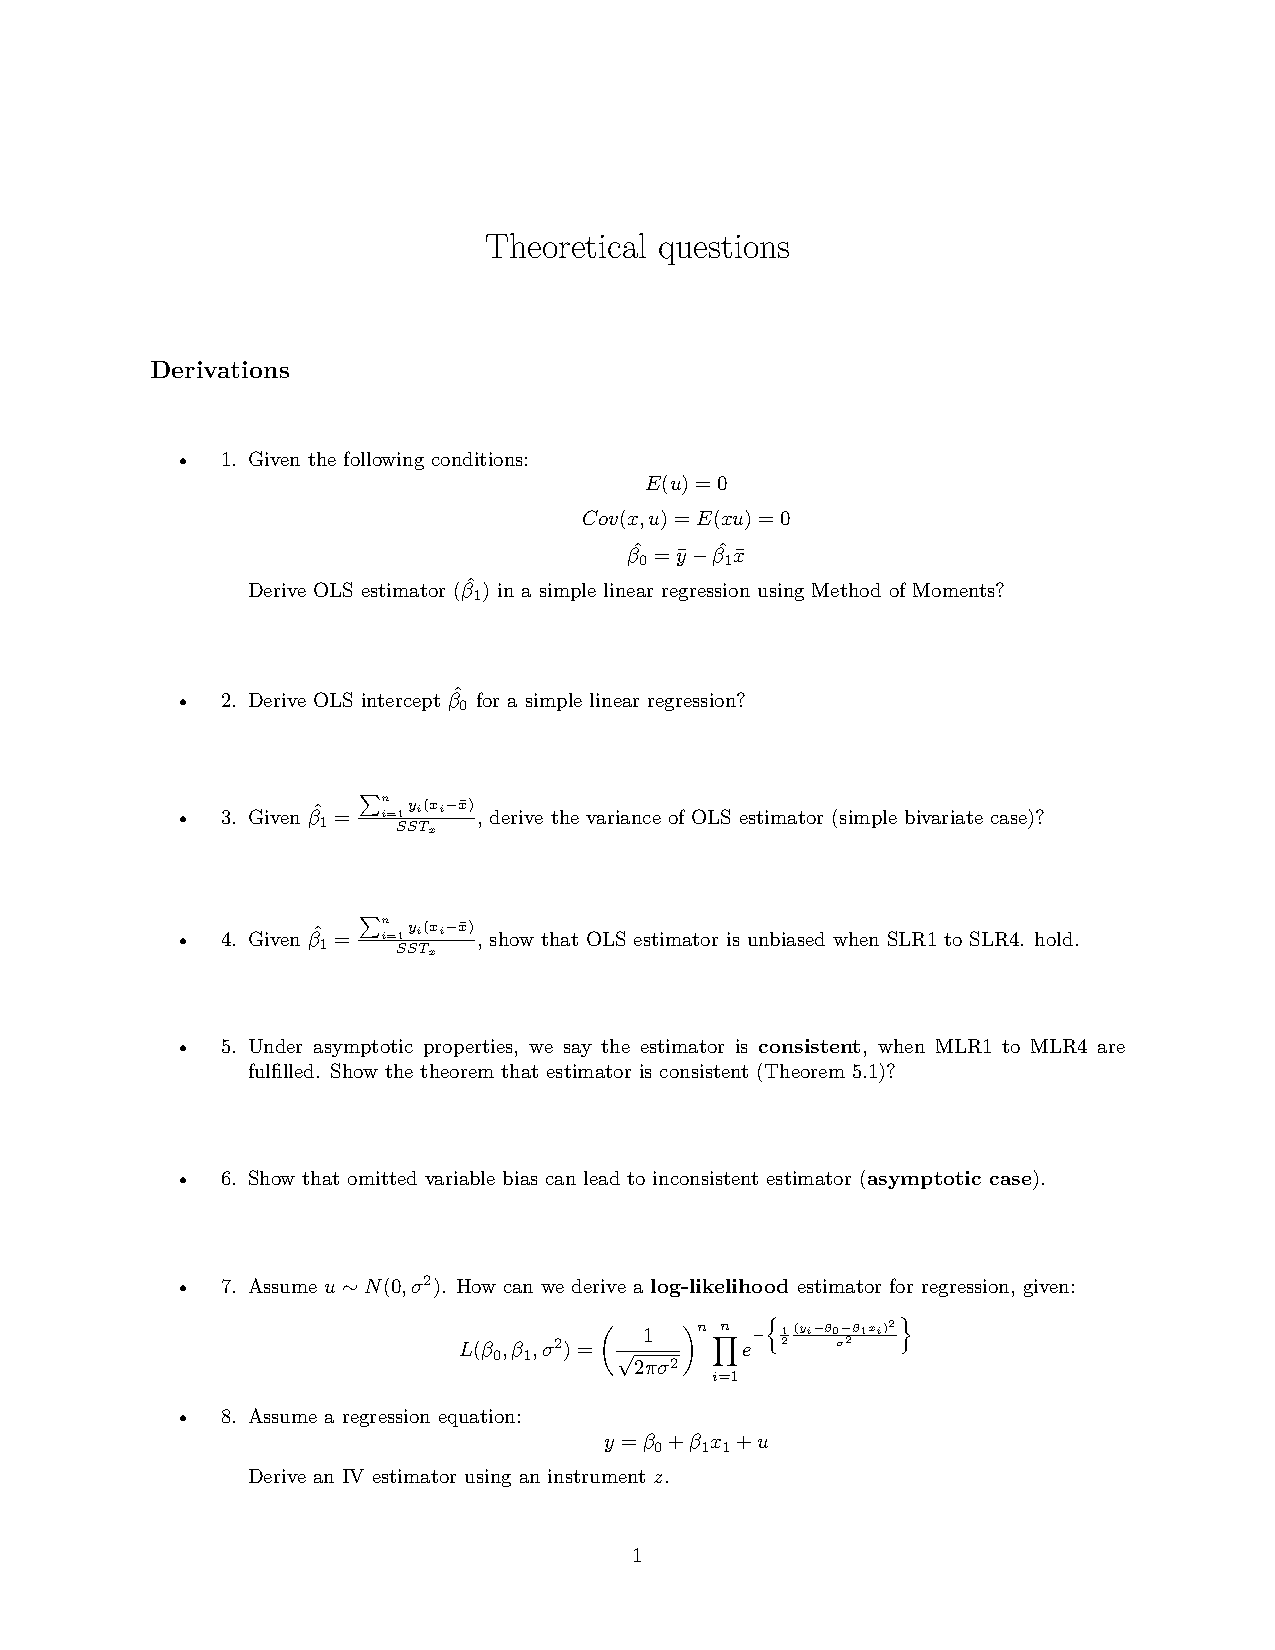
\includepdf[pages=1,pagecommand=\section{Teoretiske udledninger til eksamen}, offset=0 -0.5cm]{sporgsmal}

\hypertarget{derive-ols-estimator-hatbeta_1-in-a-simple-linear-regression-using-method-of-moments}{%
\subsubsection{\texorpdfstring{1. Derive OLS estimator
(\(\hat{\beta}_1\)) in a simple linear regression using Method of
Moments?}{1. Derive OLS estimator (\textbackslash hat\{\textbackslash beta\}\_1) in a simple linear regression using Method of Moments?}}\label{derive-ols-estimator-hatbeta_1-in-a-simple-linear-regression-using-method-of-moments}}

\leavevmode

Vi får givet følgende betingelser: \[ E(u)=0\] \[ Cov(x,u)=E(xu)=0\]
\[ \hat{\beta_0} = \bar{y}-\hat{\beta_1\bar{x}} \]

\textbf{Udledning af $\hat{\beta_1}$:}\\
Indsætter vores u værdi: \[E[x(y-\beta_0-\beta_1x)]=0\]
\[\text{Da}\ u=y-\beta_0-\beta_1x <=> y=\beta_0+\beta_1x+u  \] Ganger
\(E[x]\) ind i parantesen: \[E(xy)-E(\beta_0)x-E(\beta_1x^2)=0 \] Går
fra populationsbetingelse til stikprøve betingelse
\[\tfrac{1}{n}\sum\limits_{i=1}^n x_iy_i-\hat{\beta_0}\tfrac{1}{n}\sum\limits_{i=1}^nx_i-\hat{\beta_1}\tfrac{1}{n}\sum\limits_{i=1}^nx_i^2\]
Bruger nu \(\hat{\beta_0}\) fra betingelserne og indsætter:
\[\tfrac{1}{n}\sum\limits_{i=1}^n x_iy_i-(\bar{y}-\hat{\beta_1}\bar{x})\tfrac{1}{n}\sum\limits_{i=1}^nx_i-\hat{\beta_1}\tfrac{1}{n}\sum\limits_{i=1}^nx_i^2\]
Vi kan undlade \(\frac{1}{n}\) fra ligningen:
\[\sum\limits_{i=1}^n x_iy_i-(\bar{y}-\hat{\beta_1}\bar{x})\sum\limits_{i=1}^nx_i-\hat{\beta_1}\sum\limits_{i=1}^nx_i^2\]
Ophæver paranteserne:
\[\sum\limits_{i=1}^n x_iy_i+\hat{\beta_1}\bar{x}\sum\limits_{i=1}^nx_i-\bar{y}\sum\limits_{i=1}^nx_i-\hat{\beta_1}\sum\limits_{i=1}^nx_i^2\]
\textbf{Nu kan vi løse modellen for $\hat{\beta_1}$ ved at isolere for $\hat{\beta_1}$ :}
\[\sum\limits_{i=1}^nx_iy_i-\bar{y}\sum\limits_{i=1}^n x_i-\hat{\beta_1}\sum\limits_{i=1}^n x_i^2+\hat{\beta_1}\bar{x}\sum\limits_{i=1}^nx_i = 0\]
Reducerer og hiver \(\hat{\beta_1}\) uden for parantes:
\[\sum\limits_{i=1}^nx_iy_i-\bar{y}\sum\limits_{i=1}^n x_i-\hat{\beta_1}(\sum\limits_{i=1}^n x_i^2+\bar{x}\sum\limits_{i=1}^nx_i) = 0\]
Vi kan nu isolere \(\hat{\beta_1}\) på venstre side af lighedstegnet og
forkorte ved reduktion af vores summeringstegn og sætte \(x_i\) uden for
parantes:
\[\hat{\beta_1}= \frac{\sum\limits_{i=1}^nx_iy_i-\bar{y}\sum\limits_{i=1}^n x_i}{\sum\limits_{i=1}^n x_i^2+\bar{x}\sum\limits_{i=1}^nx_i}....\hat{\beta_1}= \frac{\sum\limits_{i=1}^nx_i(y_i-\bar{y})}{\sum\limits_{i=1}^n x_i(x_i-\bar{x})} \]
Da vi kender følgende regneregler:
\[\sum\limits_{i=1}^nx_i(y_i-\bar{y})=\sum\limits_{i=1}^n(x_i-\bar{x})(y_i-\bar{y}) \tag{a}\]
\[\sum\limits_{i=1}^nx_i(x_i-\bar{x})=\sum\limits_{i=1}^n=(x_i-\bar{x})^2 \tag{b} \]
Så kan \(\hat{\beta_1}\) blive skrevet på følgende måde:
\[\hat{\beta_1}= \frac{\sum\limits_{i=1}^n(x_i-\bar{x})(y_i-\bar{y})}{\sum\limits_{i=1}^n(x_i-\bar{x})^2}\]
Vi har nu udledt OLS, hvor \(\hat{\beta_1}\) er lig stikprøve
kovariansen mellem x og y, divideret med stikprøve variansen for x.
\newpage

\hypertarget{derive-ols-intercept-hatbeta_0-for-a-simple-linear-regression}{%
\subsubsection{\texorpdfstring{2. Derive OLS intercept \(\hat{\beta_0}\)
for a simple linear
regression?}{2. Derive OLS intercept \textbackslash hat\{\textbackslash beta\_0\} for a simple linear regression?}}\label{derive-ols-intercept-hatbeta_0-for-a-simple-linear-regression}}

\leavevmode

Vi har følgende betingelser: \[ E(u)=0\] \[ Cov(x,u)=E(xu)=0\] Vi
starter med at sætte u ind i \(E(u)\): \[E[x(y-\beta_0-\beta_1x)]=0\]
\[\text{Da}\ u=y-\beta_0-\beta_1x <=> y=\beta_0+\beta_1x+u  \] Ganger
\(E[x]\) ind i parantesen: \[E(xy)-E(\beta_0)x-E(\beta_1x^2)=0 \] Nu går
vi fra en populationsbetingelse til en stikprøve betingelse.
\[\tfrac{1}{n}\sum\limits_{i=1}^n y_i-\hat{\beta_0}-\hat{\beta_1}\tfrac{1}{n}\sum\limits_{i=1}^n x_i=0 \]
Vi kender vi følgende:
\[ \bar{y} = \tfrac{1}{n}\sum\limits_{i=1}^n y_i \]
\[ \bar{x} = \tfrac{1}{n}\sum\limits_{i=1}^n x_i \] og kan derfor
omskrive til: \[ \bar{y}- \hat{\beta_0}-\hat{\beta_1}\bar{x}=0 \] Kan nu
isolere for \(\hat{\beta_0}\)
\[ \hat{\beta_0} = \bar{y}-\hat{\beta_1}\bar{x} \] Nu har vi udledt
\(\hat{\beta_0}\), som er vores intercept i regressionensmodellen, og
som også bruges i udlednigen af \(\hat{\beta_1}\) \newpage

\hypertarget{derive-the-variance-of-ols-estimator-simple-bivariate-case}{%
\subsubsection{3. Derive the variance of OLS estimator (simple bivariate
case)?}\label{derive-the-variance-of-ols-estimator-simple-bivariate-case}}

\leavevmode

Vi får givet følgende:
\[ \hat{\beta_1}=\frac{\sum\limits_{i=1}^n y_i(x_1-\bar{x})}{SST_x}\] Så
tager vi udgangspunkt i en standard regressions model:
\[y_i=\beta_0+\beta_1x_i+u_i \] og indsætter denne i udgangspunktet
\[ \hat{\beta_1}=\frac{\sum\limits_{i=1}^n (x_i-\bar{x})(\beta_0+\beta_1x_i+u_i)}{SST_x} \]
Vi ophæver højre brøk i tælleren.
\[ \hat\beta_1 =\frac{\sum\limits_{i=1}^n (x_i-\bar{x})\beta_0 +\sum\limits_{i=1}^n (x_i-\bar{x})\beta_1x_i+\sum\limits_{i=1}^n (x_1-\bar{x})u_i} {SST_x} \]
Vi isolerer betaerne på venstre side af summeringstegnet
\[ \hat\beta_1 =\frac{\beta_0\sum\limits_{i=1}^n (x_i-\bar{x}) +\beta_1\sum\limits_{i=1}^n (x_i-\bar{x})x_i+\sum\limits_{i=1}^n (x_i-\bar{x})u_i} {SST_x} \]
Nu kender vi nogle udtryk: \[\sum\limits_{i=1}^n (x_i-\bar{x})=0\ \]
\[\text{Da}\\\ \sum\limits_{i=1}^n (x_i-\bar{x}) = \sum\limits_{i=1}^n x_i-\bar{x} \sum\limits_{i=1}^n 1=\sum\limits_{i=1}^n x_i-\bar{x}n= \bar{x}n-\bar{x}n=0 \]
og vi kender
\[\sum\limits_{i=1}^n (x_i-\bar{x})x_i=\sum\limits_{i=1}^n (x_i-\bar{x})^2=SST_x \]
\[\text{Da} \\\
\sum\limits_{i=1}^n (x_i-\bar{x})x_i = \sum\limits_{i=1}^n (x_i-\bar{x})(x_i-\bar{x})=\sum\limits_{i=1}^n (x_i-\bar{x})^2=SST_x \]
Nu kan vi sætte vores udtryk ind i den oprindelige ligning:
\[\hat\beta_1 =\frac{\beta_1 SST_X+\sum\limits_{i=1}^n (x_1-\bar{x})u_i}{SST_X} \]
Lader \(SST_x\) gå ud med hinanden:
\[\hat\beta_1 =\beta_1+\frac{ \sum\limits_{i=1}^n (x_1-\bar{x})u_i}{SST_X} \]
Dette kan omskries til
\[\hat\beta_1=\beta_1+\frac{1}{SST_x}\sum\limits_{i=1}^n(x_i-\bar{x})u_i \]
Nu tager vi variansen og bruger reglerne \(Var(a)=0\), og
\(Var(aX)=a^2Var(X)\). Da vi ved, at
\(\frac{1}{SST_x}\sum\limits_{i=1}^n(x_i-\bar{x})\) er faste værdier,
kan vi bruge ovenstående regler:
\[Var(\hat\beta_1) =0 +\left(\frac{1}{SST_x}\right)^2\sum\limits_{i=1}^n(x_i-\bar{x})^2Var(u_i) \]
Vi ved at: \(\sum\limits_{i=1}^n(x_i-\bar{x})^2 = SST_x\), så vi ganger
ind i parantesen: \[Var(\hat\beta_1) =\frac{1}{SST_x}Var(u_i) \] Nu ved
vi at \(Var(u_i|x_i)=\sigma^2\), så vi kan skrive:
\[Var(\hat\beta_1) =\frac{1}{SST_x}\sigma^2\]

\newpage

\hypertarget{show-the-ols-estimator-is-unbiased-when-slr1-to-slr4.-hold.}{%
\subsubsection{4. Show the OLS estimator is unbiased when SLR1 to SLR4.
hold.}\label{show-the-ols-estimator-is-unbiased-when-slr1-to-slr4.-hold.}}

Vi får givet følgende:
\[ \hat{\beta_1}=\frac{\sum\limits_{i=1}^n y_i(x_1-\bar{x})}{SST_x}\] Så
tager vi udgangspunkt i en standard regressions model:
\[y_i=\beta_0+\beta_1x_i+u_i \] og indsætter denne i udgangspunktet
\[ \hat{\beta_1}=\frac{\sum\limits_{i=1}^n (x_i-\bar{x})(\beta_0+\beta_1x_i+u_i)}{SST_x} \]
Vi ophæver højre brøk i tælleren.
\[ \hat\beta_1 =\frac{\sum\limits_{i=1}^n (x_i-\bar{x})\beta_0 +\sum\limits_{i=1}^n (x_i-\bar{x})\beta_1x_i+\sum\limits_{i=1}^n (x_1-\bar{x})u_i} {SST_x} \]
Vi isolerer betaerne på venstre side af summeringstegnet
\[ \hat\beta_1 =\frac{\beta_0\sum\limits_{i=1}^n (x_i-\bar{x}) +\beta_1\sum\limits_{i=1}^n (x_i-\bar{x})x_i+\sum\limits_{i=1}^n (x_i-\bar{x})u_i} {SST_x} \]
Nu kender vi nogle udtryk: \[\sum\limits_{i=1}^n (x_i-\bar{x})=0\ \]
\[\text{Da}\\\ \sum\limits_{i=1}^n (x_i-\bar{x}) = \sum\limits_{i=1}^n x_i-\bar{x} \sum\limits_{i=1}^n 1=\sum\limits_{i=1}^n x_i-\bar{x}n= \bar{x}n-\bar{x}n=0 \]
og vi kender
\[\sum\limits_{i=1}^n (x_i-\bar{x})x_i=\sum\limits_{i=1}^n (x_i-\bar{x})^2=SST_x \]
\[\text{Da} \\\
\sum\limits_{i=1}^n (x_i-\bar{x})x_i = \sum\limits_{i=1}^n (x_i-\bar{x})(x_i-\bar{x})=\sum\limits_{i=1}^n (x_i-\bar{x})^2=SST_x \]
Nu kan vi sætte vores udtryk ind i den oprindelige ligning:
\[\hat\beta_1 =\frac{\beta_1 SST_X+\sum\limits_{i=1}^n (x_1-\bar{x})u_i}{SST_X} \]
Lader \(SST_x\) gå ud med hinanden:
\[\hat\beta_1 =\beta_1+\frac{ \sum\limits_{i=1}^n (x_1-\bar{x})u_i}{SST_X} \]
Dette kan omskrives til:
\[\hat\beta_1=\beta_1+\left(\frac{1}{SST_x}\right)\sum\limits_{i=1}^nd_iu_i \]
\[ \text{Hvor}\ d_i =(x_i-\bar{x})\] Nu kan vi anvende SLR4.
\(E(u_i|x_i)=0\)
\[ E(\hat\beta_1)=E(\beta_1)=E\left[(\frac{1}{SST_x})\sum\limits_{i=1}^nd_iu_i\right]\]
Da vi ved, at \(E[u_i]=0\) så: \[\hat\beta_1=\beta_1+0\] \newpage

\hypertarget{under-asymptotic-properties-we-say-the-estimator-is-consistent-when-mlr1-to-mlr4-are-fulfilled.-show-the-theorem-that-estimator-is-consistent-theorem-5.1}{%
\subsubsection{5. Under asymptotic properties, we say the estimator is
consistent, when MLR1 to MLR4 are fulfilled. Show the theorem that
estimator is consistent (Theorem
5.1)?}\label{under-asymptotic-properties-we-say-the-estimator-is-consistent-when-mlr1-to-mlr4-are-fulfilled.-show-the-theorem-that-estimator-is-consistent-theorem-5.1}}

\leavevmode
\begin{mytheo}{Theorem 5.1}{theorem}
 Teoremet siger, at under antagelserne MLR1 til MLR4 er OLS estimatoren $\hat\beta_j$ konsistent for $\beta_j$, for alle $j=0,1,...,k$.
\end{mytheo}

Vi viser Theorem 5.1, som er givet vores \(\hat\beta_1\) på forhånd:
\[\hat{\beta_1}= \frac{\sum\limits_{i=1}^n(x_{i1}-\bar{x})y_i}{\sum\limits_{i=1}^n(x_{i1}-\bar{x})^2}\]
Vi indsætter vores regressionsmodel \(y_1=\beta_0+\beta_1x_{i1}+u_i\)
\[\hat{\beta_1}= \beta_1+\frac{n^{-1}\sum\limits_{i=1}^n(x_{i1}-\bar{x})u_i}{n^{-1}\sum\limits_{i=1}^n(x_{i1}-\bar{x})^2}\]
Når man dividerer både tæller og nævner med \(n^{-1}\) giver det os ikke
en forskel, men vi kan istedet bruge Law of large numbers.\\
Så konvergerer hhv. nævneren og tælleren mod sandsynlighederne for
populationsmængderne. Så:
\[ n^{-1}\sum\limits_{i=1}^n(x_{i1}-\bar{x})u_i\ \text{mod}\ Cov(x_1,u)\]
og
\[n^{-1}\sum\limits_{i=1}^n(x_{i1}-\bar{x})^2\ \text{mod}\ Var(x_1) \] i
MLR3 er det givet at \(Var(x_1)\neq0\), og vi kan derfor bruge
sandsynlighedsgrænser for at få følgende:
\[ plim\ \beta_1 =\beta_1+\frac{Cov(x_1,u)}{Var(x_1)} = \beta_1\ \text{da}\ Cov(x_1,u)=0\]
\(x_1\) og \(u\) har ingen kovarians. Dette er antaget i MLR4. \newpage

\hypertarget{show-that-omitted-variable-bias-can-lead-to-inconsistent-estimator-asymptotic-case.}{%
\subsubsection{6. Show that omitted variable bias can lead to
inconsistent estimator (asymptotic
case).}\label{show-that-omitted-variable-bias-can-lead-to-inconsistent-estimator-asymptotic-case.}}

\leavevmode

Her har vi givet følgende: \[y=\beta_0+\beta_1x_1+\beta_2x_2+u \] Her
antager vi, at vi har glemt en variabel \(x_2\) i vores regression.
\[ y=\tilde\beta_0+\tilde{\beta_1}x_1+u\] Derfor kan det vises at:
\[\tilde{\beta_1}=\beta_1+\delta_1\beta_2\] og vi får derfor følgende:
\[\delta_1=\frac{Cov(x_1,x_2)}{Var(x_1)}\] Det vil altså sige, at hvis
\(\delta\neq0\) så har det at udelade \(x_2\) for vores model skabt bias
i modellen. Det betyder, at vi får inkonsistente estimatorer. \newpage

\hypertarget{how-can-we-derive-a-log-likelihood-estimator-for-regression.}{%
\subsubsection{7. How can we derive a log-likelihood estimator for
regression.}\label{how-can-we-derive-a-log-likelihood-estimator-for-regression.}}

Vi antager, at vi har en normalfordeling: \[ u\sim N(0,\sigma^2) \] Hvor
det er givet:
\[ L(\beta_0, \beta_1,\sigma^2)=\left(\frac{1}{\sqrt2\pi\sigma^2}\right)^n\prod\limits_{i=1}^n e^{-\left\{\frac{1}{2}\frac{(y_i-\beta_0-\beta_1x_i)^2}{\sigma^2}  \right\}} \]
Nu tager vi log på begge sider af:
\[ logL(\beta_0, \beta_1,\sigma^2)=log\left[\left(\frac{1}{\sqrt2\pi\sigma^2}\right)^n\prod\limits_{i=1}^n e^{-\left\{\frac{1}{2}\frac{(y_i-\beta_0-\beta_1x_i)^2}{\sigma^2}  \right\}}\right] \]
Når man tager log af et produkt(\(\prod\)), så bliver det til et sum
tegn, plus vores \(e\) forsvinder, og vi rykker minustegnet ud foran
sumtegnet:
\[logL(\beta_0, \beta_1,\sigma^2)=log\left(\frac{1}{\sqrt2\pi\sigma^2}\right)^n-\sum\limits_{i=1}^n {\left\{\frac{1}{2}\frac{(y_i-\beta_0-\beta_1x_i)^2}{\sigma^2}  \right\}} \]
Trækker \(n\) ud foran første led og \(\frac{1}{2}\) ud foran sumtegnet.
\[logL(\beta_0, \beta_1,\sigma^2)= -\frac{n}{2}log(2\pi\sigma^2)-\frac{1}{2}\sum\limits_{i=1}^n\frac{(y_i-\beta_0-\beta_1x_i)^2}{\sigma^2} \]
Nu lader vi \(\sigma^2\) være givet, så vi kan maksimere i henhold til
\(\beta_0\) og \(\beta_1\)
\[logL(\beta_0, \beta_1,\sigma^2)= -\frac{n}{2}log(2\pi\sigma^2)-\frac{1}{2\sigma^2}\sum\limits_{i=1}^n(y_i-\beta_0-\beta_1x_i)^2 \]
Nu har vi den udledte funktion og kan så tage første ordens betingelsen
i henhold til \(\beta_0\): Så først ganger vi igennem med (-1) og så
tager vi FOC til \(\beta_0\)
\[logL(\beta_0, \beta_1,\sigma^2)= \frac{n}{2}log(2\pi\sigma^2)\frac{1}{2\sigma^2}\sum\limits_{i=1}^n(y_i-\beta_0-\beta_1x_i)^2 \]
Vi ved at \(\frac{n}{2}log(2\pi\sigma^2)\) er en konstant så ved partiel
differention fås:
\[ \frac{\partial logL(\beta_0,\beta_1,\sigma^2)}{\partial\hat{\beta_0}}=\frac {2} {2\sigma^2}\sum\limits_{i=1}^n(y_i-\beta_0-\beta_1x_i)\]
\(\frac{2}{2\sigma^2}\) fjernes:
\[ \frac{\partial logL(\beta_0,\beta_1,\sigma^2)}{\partial\hat{\beta_0}}=\sum\limits_{i=1}^n(y_i-\beta_0-\beta_1x_i)\]
Nu kan vi tage FOC til \(\beta_1\)
\[ \frac{\partial logL(\beta_0,\beta_1,\sigma^2)}{\partial\hat{\beta_0}}=\sum\limits_{i=1}^n(y_i-\beta_0-\beta_1x_i)\]
vi bruger intercept(\(\beta_0\)) ligningen:
\[\hat{\beta_0}=\bar{y}-\hat{\beta_1}\bar{x} \] Indsættes i ligningen
fra før:
\[ \frac{\partial logL(\beta_0,\beta_1,\sigma^2)}{\partial\hat{\beta_0}}=\sum\limits_{i=1}^n(y_i-(\bar{y}-\hat{\beta_1}\bar{x})-\beta_1x_i)=0\]
Vi omskriver:
\[ \frac{\partial logL(\beta_0,\beta_1,\sigma^2)}{\partial\hat{\beta_0}} =\sum\limits_{i=1}^n x_i(y_i-\bar{y})-\sum\limits_{i=1}^n x_i(-\hat\beta_1\bar{x}+\hat\beta_1x_i)=0\]
\[\sum\limits_{i=1}^n x_i(-\hat\beta_1\bar{x}+\hat\beta_1x_i) =\sum\limits_{i=1}^n x_i(y_i-\bar{y})\]
Bruger reglen:
\[ \sum\limits_{i=1}^n x_i(y_i-\bar{y}) =\sum\limits_{i=1}^n(x_i-\bar{x})(y_i-\bar{y})\]
Faktoriserer \(\hat\beta_1\) ud:
\[\hat\beta_1\left(\sum\limits_{i=1}^nx_i(x_i-\bar{x})\right) =\sum\limits_{i=1}^n(x_i-\bar{x})(y_i-\bar{y})\]
Bruger reglen:
\[\sum\limits_{i=1}^nx_i(x_i-\bar{x})=\sum\limits_{i=1}^n(x_i-\bar{x})^2 \]
\[ \hat\beta_1\left( \sum\limits_{i=1}^n(x_i-\bar{x})^2 \right) = \sum\limits_{i=1}^n(x_i-\bar{x})(y_i-\bar{y}) \]
Kan nu isolere for \(\hat\beta_1\)
\[\hat\beta_1 = \frac{\sum\limits_{i=1}^n(x_i-\bar{x})(y_i-\bar{y})} {\sum\limits_{i=1}^n(x_i-\bar{x})^2} \]

Vi har nu både udledt Maximum Likelihood funktionen og dens estimaterer
\(\beta_0\) og~\(\beta_1\) \newpage

\hypertarget{derive-an-iv-estimator-using-an-instrument-z.}{%
\subsubsection{8. Derive an IV estimator using an instrument
z.}\label{derive-an-iv-estimator-using-an-instrument-z.}}

Vi har en regressionsfunktion: \[y=\beta_0+\beta_1x_1+u \] Her antages
det, at der mangler en vigtig variabel, hvilket betyder:
\[Cov(x,u)\neq0\] Nu vil vi anvende z som instrument og antager derfor:
\[ Cov(z,u)=0\] \[ Cov(z,x)\neq0\] Hvor z er instrumentvariabel for x.\\
Vi tager Cov i forhold til z på begge sider og antager at
\(Cov(\beta_0,z)=0\), samt bruger reglen: \(Cov(aX,Y)=aCov(x,y)\)\\
\[ Cov(y,z)=0+\beta_1Cov(x,z)+Cov(u,z)\] Da \(Cov(z,u)=0\) får vi:
\[ Cov(y,z)=\beta_1Cov(x,z)+0\] Nu kan vi isolere for \(\beta_1\)
\[\beta_1=\frac{Cov(y,z)}{Cov(x,z)} \] Her er det vigtigt, at
\(Cov(x,z)\neq0\) da vi ellers ville dividere med 0.\\
Vi estimerer \(\beta_1\) ved at indskrive formlerne for Kovarianserne:
\[\hat{\beta_1}= \frac{\tfrac{1}{n}\sum\limits_{i=1}^n (z_i-\bar{z})(y_i-\bar{y})}{\tfrac{1}{n}\sum\limits_{i=1}^n (z_i-\bar{z})(x_i-\bar{x})} \]
\(\frac{1}{n}\) kan nu fjernes fra både tæller og nævner:
\[\hat{\beta_1}= \frac{\sum\limits_{i=1}^n (z_i-\bar{z})(y_i-\bar{y})}{\sum\limits_{i=1}^n (z_i-\bar{z})(x_i-\bar{x})} \]
Her kan vi også se, at hvis \(z=x\), så havde det været det samme som
udledningen for OLS. \newpage

\includepdf[pages=2,pagecommand=\section{Teori og formularer til eksamen}, offset=0 -0.5cm]{sporgsmal}

\hypertarget{what-is-the-formula-of-the-total-sum-of-square-sst-of-a-variable-y-what-is-the-formula-of-the-estimated-sum-of-square-sse-of-a-variable-y-what-is-the-formula-of-the-residual-sum-of-squares-ssr}{%
\subsubsection{9. What is the formula of the total sum of square (SST)
of a variable y? What is the formula of the estimated sum of square
(SSE) of a variable y? What is the formula of the residual sum of
squares
(SSR)?}\label{what-is-the-formula-of-the-total-sum-of-square-sst-of-a-variable-y-what-is-the-formula-of-the-estimated-sum-of-square-sse-of-a-variable-y-what-is-the-formula-of-the-residual-sum-of-squares-ssr}}

\[ SST=\sum\limits_{n=i}^n(y_i-\bar{y})^2\]
\[ SSE=\sum\limits_{n=i}^n(\bar{y_i}-\bar{y})^2\]
\[ SSR=\sum\limits_{n=i}^n\hat{u}_i^2 \]

\hypertarget{what-is-the-difference-between-adjusted-r2-and-r2}{%
\subsubsection{\texorpdfstring{10. What is the difference between
adjusted \(R^2\) and \(R^2\)
?}{10. What is the difference between adjusted R\^{}2 and R\^{}2 ?}}\label{what-is-the-difference-between-adjusted-r2-and-r2}}

Adjusted \(R^2\) straffer variabler, der ikke er forklarende for
modellen. Dette gør \(adjR^2\) lavere end den normale \(R^2\). \(R^2\)
viser hvor meget højre-side variablerne(de uafhængige) forklarer den
afhængige variabel.

\hypertarget{can-you-describe-the-gauss-markov-assumptions-which-assumptions-are-required-to-show-that-ols-is-unbiasedconsistent-which-assumptions-are-required-to-show-ols-is-blue}{%
\subsubsection{11. Can you describe the Gauss-Markov assumptions? Which
assumptions are required to show that OLS is unbiased/consistent? Which
assumptions are required to show OLS is
BLUE}\label{can-you-describe-the-gauss-markov-assumptions-which-assumptions-are-required-to-show-that-ols-is-unbiasedconsistent-which-assumptions-are-required-to-show-ols-is-blue}}

SLR 1-4 bruges til at konstatere om de estimerede værdier er biased
eller unbiased.\\
SLR 1-5 skal overholdes for at OLS er BLUE.

\hypertarget{how-does-ols-estimate-the-estimators-or-what-is-the-objective-function-solved-by-ols}{%
\subsubsection{12. How does OLS estimate the estimators OR what is the
objective function solved by
OLS?}\label{how-does-ols-estimate-the-estimators-or-what-is-the-objective-function-solved-by-ols}}

OLS estimerer parameterne i en multiple linæer regression ved at
minimere summen af ``squared'' residuals. Dette betyder, at regressionen
sørger for at residualerne(fejlledene) bliver så små som muligt og så
tæt på ``OLS-regresisions-linjen'' som muligt. Det er altså et
minimeringsproblem.

\hypertarget{what-are-the-consequences-of-including-irrelevant-variables-in-a-regression}{%
\subsubsection{13. What are the consequences of including irrelevant
variables in a
regression?}\label{what-are-the-consequences-of-including-irrelevant-variables-in-a-regression}}

Det vil ikke påvirke unbiassedness for modellen, men det kan gå ind og
have negative følger for bla. varianserne på OLS estimaterne.

\hypertarget{what-are-the-consequences-of-omitting-a-relevant-variable-in-a-regression}{%
\subsubsection{14. What are the consequences of omitting a relevant
variable in a
regression?}\label{what-are-the-consequences-of-omitting-a-relevant-variable-in-a-regression}}

Der kan opstå bias i modellen, såkaldt ``omitted variable bias''. Dette
behøver ikke nødvendigvis være et problem afhængig af størrelsen af
dette. \newpage

\hypertarget{the-variance-of-the-error-term-is-represented-by-sigma2-what-is-the-formula-of-computing-sigma2}{%
\subsubsection{\texorpdfstring{15. The variance of the error term is
represented by \(\sigma^2\) , what is the formula of computing
\(\sigma^2\)}{15. The variance of the error term is represented by \textbackslash sigma\^{}2 , what is the formula of computing \textbackslash sigma\^{}2}}\label{the-variance-of-the-error-term-is-represented-by-sigma2-what-is-the-formula-of-computing-sigma2}}

Variansen af u er ukendt, men kan blive repræsenteret på følgende
formel:
\[ \sigma^2 \frac{\sum\limits_{n=i}^n(\hat{u}_i)^2}{n-(k+1)}=\frac{SSR}{n-(k+1)}\]
Hvor \((k+1)\) referer til hvor mange \(\beta\) værdier vi har, så:
\[\beta_0,\beta_1,\beta_2,...,\beta_k \] og \(n-(k+1)\) referer til
antallet af frihedsgrader.

\hypertarget{what-is-the-formula-of-t-statistics-or-t-ratio}{%
\subsubsection{16. What is the formula of t statistics or t
ratio?}\label{what-is-the-formula-of-t-statistics-or-t-ratio}}

Metoden vi bruger til at teste nulhypotesen mod den alternative hypotese
kaldes T-statistik eller t-ratio og opskrives:
\[t_{\hat{\beta_j}}=\frac{\hat{\beta_j}}{se(\hat{\beta_j)}} \] Her er
værdien \(se(\hat{\beta_j)}\) altid positiv, mens \(\beta_j\) kan være
begge dele. T-statistikkens fortegn afhænger altså af dette.

\hypertarget{what-is-right-tailed-left-tailed-and-two-sided-test}{%
\subsubsection{17. What is right tailed, left tailed, and two-sided
test?}\label{what-is-right-tailed-left-tailed-and-two-sided-test}}

\textbf{Right-tailed test:}\\
En right-tailed test er hvor nulhypotesen kunne være:
\[H_0:\beta_j\leq0 \] Og den alternative hypotese er:
\[H_1:\beta_j>0 \]\\
\textbf{left-tailed test:}\\
En left-tailed test er hvor nulhypotesen kunne være:
\[H_0:\beta_j\geq0 \] Og den alternative hypotese er:
\[H_1:\beta_j<0 \]\\
\textbf{Two-sided test:}\\
En two-sided test kunne have en nulhypotese på: \[H_0:\beta_j=0 \] Og
den alternative hypotese er: \[H_0:\beta_j\neq0 \]

\hypertarget{what-are-the-desirable-properties-of-error-term-in-ols}{%
\subsubsection{18. What are the (desirable) properties of error term in
OLS?}\label{what-are-the-desirable-properties-of-error-term-in-ols}}

Den eneste måde at få troværdige estimator på, er hvis fejlleddet(u)
ikke er relateret til x. Derfor er der to følgende antagelser:
\[ E(u)=0\] \[ E(u|x)=E(u)=0\] Hvor den sidste antagelse siger, at
middelværdien af fejlleddet(u) er uafhængig af x.

\hypertarget{what-are-the-conditions-that-instrumental-iv-should-satisfy}{%
\subsubsection{19. What are the conditions that instrumental IV should
satisfy?}\label{what-are-the-conditions-that-instrumental-iv-should-satisfy}}

Instrumentvariablen kaldes ofte for z og er en instrumentvariabel for x.
Den skal opfylde disse betingelser: \[Cov(z,u)=0 \] Hvis z er korreleret
med x, får vi: \[ Cov(z,x)\neq0\] hvilket ville skabe ``instrument
eksogenitet''.

\hypertarget{what-is-a-reduced-form-equation-in-the-context-of-iv-regressions}{%
\subsubsection{20. What is a reduced form equation in the context of IV
regressions?}\label{what-is-a-reduced-form-equation-in-the-context-of-iv-regressions}}

Vi antager en strukturel model for IV-estimation:
\[ y_1=\beta_0+\beta_1y_2+\beta_2z_1+u_1 \] Vi mistænker nu, at u
korrelerer med \(y_2\) og kan skrive en reduced form equation:
\[ y_2=\pi_0+\pi_1z_1+\pi_2z_2+v_2\]

\hypertarget{what-is-the-difference-between-just-identified-and-over-identified-model-in-the-context-of-iv-regression}{%
\subsubsection{21. What is the difference between `just identified' and
`over identified model' in the context of IV
regression?}\label{what-is-the-difference-between-just-identified-and-over-identified-model-in-the-context-of-iv-regression}}

\textbf{"Over indetified model":}\\
Overidentifikationstesten kan bruges, når vi har flere instrumenter end
vi behøver. Dette kan vi fordi modellen er ``over identified''.\\
\textbf{"Just indentifed":}\\
I denne model har vi lige akurat nok instrumenter, og det siges, at den
er ``just identified''. Her kan vi ikke bruge overidentifikationstesten.

\hypertarget{what-is-the-difference-between-the-equations-of-ols-and-iv-estimators-write-the-two-equations}{%
\subsubsection{22. What is the difference between the equations of OLS
and IV estimators (write the two
equations)?}\label{what-is-the-difference-between-the-equations-of-ols-and-iv-estimators-write-the-two-equations}}

\textbf{OLS estimators:}\\
\[\hat{\beta_1}= \frac{\sum\limits_{i=1}^n(x_i-\bar{x})(y_i-\bar{y})}{\sum\limits_{i=1}^n(x_i-\bar{x})^2}\]
\(\hat{\beta_1}\) er lig stikprøve kovariansen mellem x og y, divideret
med stikprøve variansen for x.\\

\textbf{IV estimators:}\\
\[ \frac{\sum\limits_{i=1}^n (z_i-\bar{z})(y_i-\bar{y})}{\sum\limits_{i=1}^n (z_i-\bar{z})(x_i-\bar{x})} \]
Her kan vi se, at \(\hat{\beta_1}\) er lig stikprøve kovariansen mellem
z og y, divideret med stikprøve kovariansen mellem z og x, også noteret:
\[ \beta_1=\frac{Cov(x,y)}{Cov(x,z)}\] Dog kan vi se, at hvis \(z=x\),
så havde IV-estimatoren været det samme som OLS estimatoren.

\hypertarget{what-are-logit-and-probit-regressions-what-are-average-partial-effects-ape-and-partial-effects-at-average-pea}{%
\subsubsection{23. What are logit and probit regressions? What are
average partial effects (APE) and partial effects at average
(PEA)?}\label{what-are-logit-and-probit-regressions-what-are-average-partial-effects-ape-and-partial-effects-at-average-pea}}

\textbf{Logit-model} Det er en regression, hvor den afhængige
variable(y), er binær, altså hvor y kun kan tage to værdier. Det samme
gør sig gældende for de uafhængige variable(x). Hvor en diskret variable
tager værdien ''1'' ved succes, og ''0'' ved fail. Det kunne være at gå
på universitet(1) eller ikke at gå på universtitet(0). En kontinuert
variable vil kun kunne tage værdier mellem 1 og 0. Det kunne være
indkomst hvor den rigeste har værdien 1, og den fattigeste har værdien
0.\\
\newline \textbf{Probit-model} Det er en regression, hvor den afhængige
variable(y) kun kan tage to værdier. Det kan være at gå på
universitet(1), eller at man ikke går på universitet(0). Vi bruger
probit-modellen til at estimere sandsynligheden for, at en observation
vil falde indenfor den ene eller den anden gruppe.\\
\newline \textbf{Partial effect at the average(PEA):}\\
Ved PEA udregner vi den partielle effekt af den gennemsnitlige variable.
Formlen for PEA er følgende:
\[ P\hat{E}A_j=g(\bar{x}\hat{\beta})\hat{\beta}_j, \ hvor\ \bar{x}=(x_1,x_2,...,x_i)\ og\ \hat{\beta}=(\beta_1,\beta_2,...\beta_i)\]
Der er også problemer forbundet med at bruge PEA. Den første er, at hvis
en eller flere af de forklarende variable er diskrete, så vil
gennemsnittet ikke repræsentere nogen af dem i stikprøven. Et eksempel
kunne være hvis \(x_1\) angiver en dummy variable for kvinder, og 47.5\%
er kvinder i stikprøven, så vil det ikke give meget mening at sætte
\(\bar{x}\)=0.475 in i formlen for det siger ikke noget om den
gennemsnitlige person. Det andet problem er, at hvis der er kontinuerte
forklarende variable viser sig at være af nonlinear funktion, det kunne
fx være, at variablen er sat i anden. Et eksempel kunne være vi har
\(x_1\) til at angive indkomst, men at \(x_2\) angiver \(indkomst^2\),
hvilken en skal vi så bruge til vores model?\\
\newline
\textbf{Average partial effect(APE) kaldes også for Average marginal effect(AME):}\\
APE tager effekten af hver enkelt obseration og finder den
gennemsnitlige effekt på tværs af disse. Det udregnes ud fra formlen:
\[A\hat{P}Ej=\hat{\beta_j}\left[n^{-1}\sum\limits_{i=1}^ng(\mathbf{x_i}\hat{\beta})\right],\ hvor\ \mathbf{x_i}=(x_1,x_2,...,x_i)\ og\ \hat{\beta}=(\beta_1,\beta_2,...\beta_i) \]\\
\textbf{Sammenligning af PEA og APE}\\
Hvor PEA udregner den gennemsnitlige observation, så kan der være
problemer hvis vi ser på en dummy variable, da det kan være besværligt
at udregne gennemsnittet. APE har ikke samme problem, da vi ved APE
udregner effekten af hver enkelt individuel observation og derefter
tager gennemsnittet af effekten. Det er grunden til vi vil foretrække
APE fremfor PEA.

\end{document}
